\begin{appendices}
	\chapter{UNC-16 regulates microtubule and actin dynamics post-injury}
	
	
	\large \textbf{UNC-16 alters DLK-1 localization and negatively regulates actin and microtubule dynamics in \textit{Caenorhabditis elegans} regenerating neurons}
	
	\small
	Sucheta S Kulkarni, \textbf{Vidur Sabharwal}, Seema Sheoran, Atrayee Basu, Kunihiro Matsumoto, Naoki Hisamoto, Anindya Ghosh-Roy, Sandhya P Koushika
	
	Publication date : 1 November 2021
	Journal : Genetics
	Volume : 219
	Issue : 3
	doi : \href{https://doi.org/10.1093/genetics/iyab139}{10.1093/genetics/iyab139}
	
	\normalsize
	My contributions to the following study include 
	1) strain building, 
	2) live imaging of microtubule and actin dynamics post neuronal injury, 
	3) analysis and quantitation of microtubule and dynamics in various mutants.
	Any figure reused from this article is authorized via the Oxford University Press license number 5598701300749.
	
	\pagebreak
	\section{Introduction} 
	
	Neurons can undergo regrowth and repair following injury. This regrowth and repair is executed by several steps post injury including sensing injury \parencite{hammarlund2009}, relaying injury signal to the nucleus \parencite{sung2001}, changes in protein activation and synthesis at the cut site \parencite{yan2009, ghosh-roy2012}, alteration of the neuronal transcriptome \parencite{jin2022}, initiation of regrowth \parencite{barnat2010}, directed growth towards the separated fragment \parencite{chisholm2016}, detection of the injury fragment \parencite{abay2017}, and finally fusion of the 2 fragments associated and dissociated from the cell body \parencite{neumann2015}.
	
	UNC-16 was found as one of the minority genes that act as repressors of regeneration in two independent screens, which aimed to find potential regulators of neuronal regeneration post injury \parencite{chen2011, nix2014}. UNC-16, the \textit{C. elegans}  orthologue of mammalian JIP3, is known to act as a scaffold for the MAPK cascade proteins \parencite{kelkar2000, senguptaghosh2011}. MAPK proteins are involved in multiple steps following neuronal injury to induce outgrowth \parencite{barnat2010, hammarlund2009, sung2001, yan2009}. How UNC-16 regulates regeneration was unclear.
	
	In this paper, I show an increase in microtubule dynamics in the proximity of the cut site, along with an increase in actin dynamics throughout the neuronal process post injury in \textit{unc-16(lf)}, which depended on \textit{dlk-1}. Thus, \textit{unc-16} may act through \textit{dlk-1} to control regeneration, likely by keeping actin and microtubule dynamics in check. Regulation by \textit{unc-16} is likely important to maintain directional outgrowth towards the dissociated fragment, increasing the probability of distal fragment fusion, thereby recovering worm behaviour.
	
	\section{Material and methods}
	
	\subsection{Measurement of actin and microtubule dynamics}

	Laser axotomy was performed using a ns-pulsed Nd-YAG LASER at 355 nm (Litron Nano S60-30) using a 60$\times$/1.35 N.A. objective. The axotomy was performed on \textit{juIs338} or \textit{wyIs291} L4 animals 100 $\mu$m from the cell body. The animals were washed with M9 buffer and rescued. At the reported time point, the animals were anesthetized with 5 mM tetramisole and imaged using 488 nm excitation with a Yokogawa CSU-X1 spinning disc confocal head and a Hamamatsu C1900-13 EMCCD camera controlled by Volocity collectively supplied by PerkinElmer. Imaging was done under a 100$\times$/1.4 N.A. objective using 300 ms exposure at 3 frames/s for a total of 3 min for \textit{juIs338} and 600 ms exposure at 1.6 frames/s for a total of 3 min for \textit{wyIs291}. Kymographs were generated using ImageJ plugin MultiKymograph \parencite{schindelin2012}. We measure the total number of EBP-2::GFP comets which are visualized as sloped lines in kymographs. The sloped lines were also used to calculate the length and direction of the comets. We measure three parameters, that are the density of stationary actin-rich regions, the number of actin trails, and actin trail length \parencite{ganguly2015, sakamoto2005}. EBP-2::GFP comets and GFP::utCH trails were then normalized to the duration of the kymograph as well as the length of the ROI to generate the normalized dynamics graph. 
			
	\section{Results}
	
	\subsection{Microtubule dynamics increase 3 hrs post injury}
	
	Previous studies have shown that microtubule dynamics are elevated 3 hours post injury \parencite{ghosh-roy2012}. We sought out to address how long after injury do microtubule dynamics start increasing. For this, we assessed microtubule dynamics using the microtubule plus-end binding protein EBP-2. The number of EBP-2::GFP trails significantly increased only 3 hours post injury [Fig.~\ref{fig:MTdyntime}A]. The EBP-2::GFP trail velocity was largely similar across all time points [Fig.~\ref{fig:MTdyntime}B], while the EBP-2::GFP trail growth length increased within 2 hours post injury [Fig.~\ref{fig:MTdyntime}C]. Thus, there was a clear hierarchy in the alterations of microtubule dynamics, with growth length increasing first after injury, followed by the number of tracks, while the polymerization velocity likely remains the same.
		

	

	
		\begin{figure}[H]
		\centering
		\begin{subfigure}{0.3\textwidth}
			\caption{}
			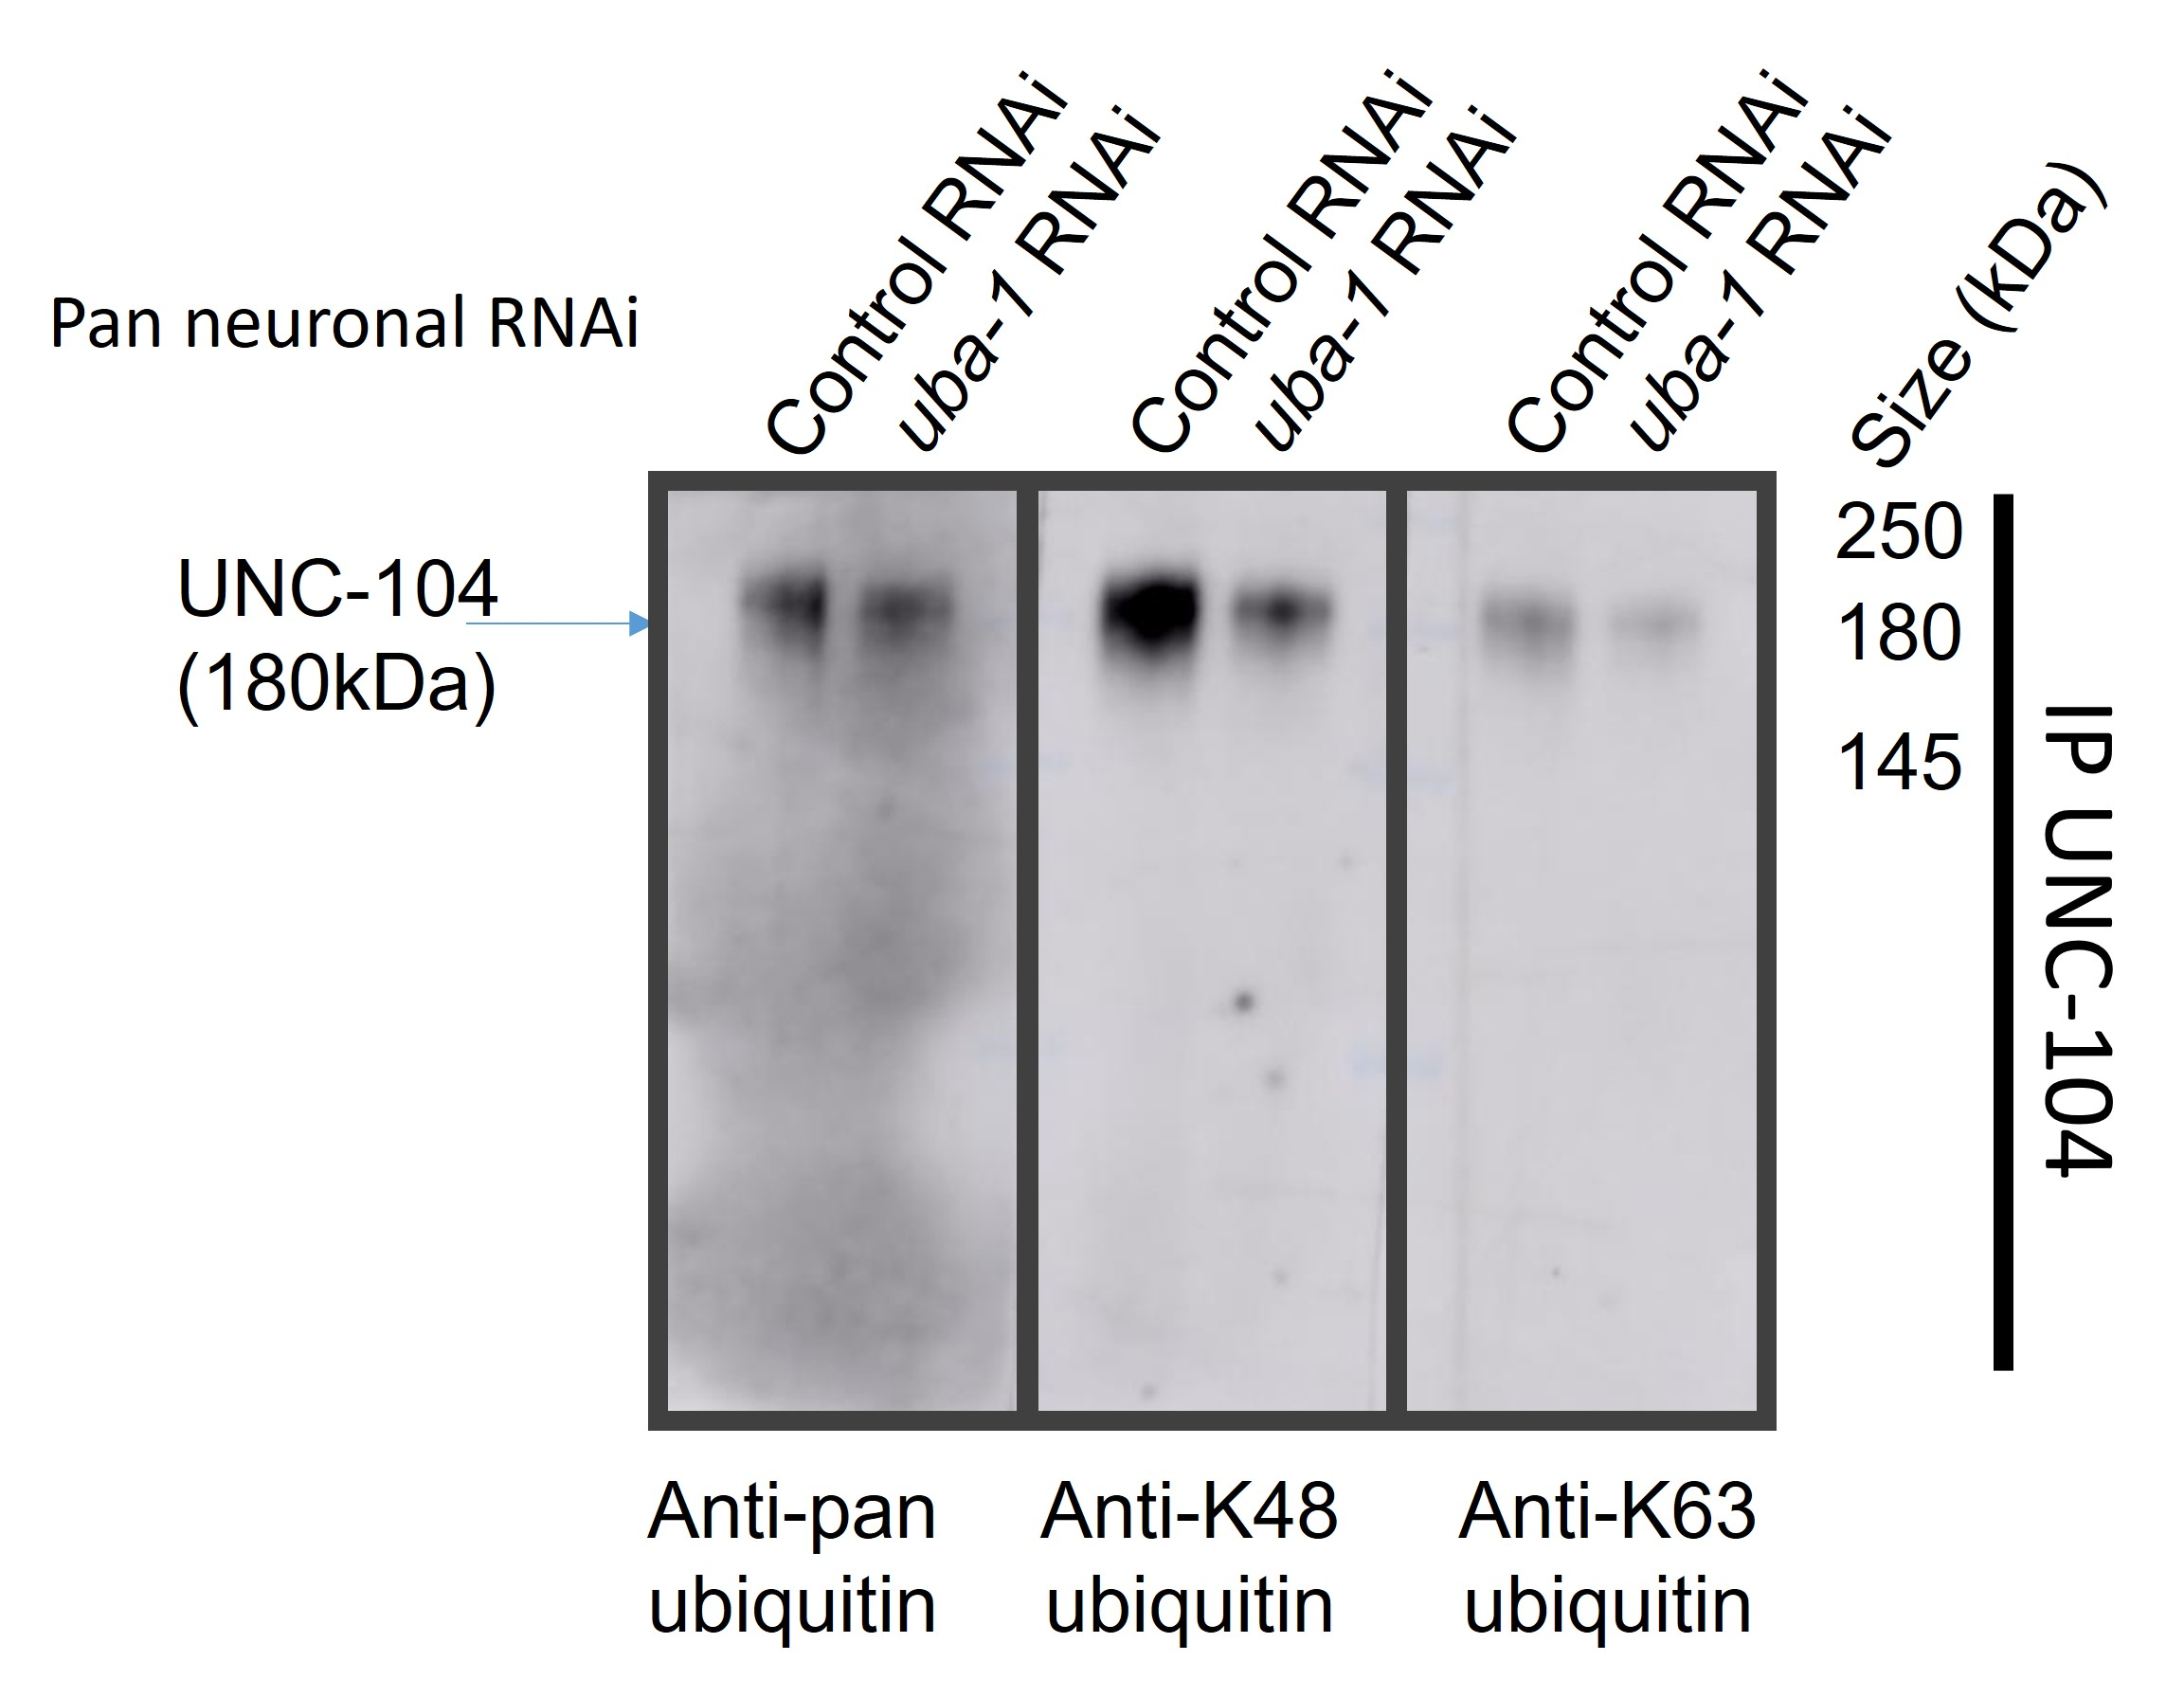
\includegraphics[width=\textwidth]{figs/example}
			
		\end{subfigure}
		%	\hfill
		\begin{subfigure}{0.3\textwidth}
			\caption{}
			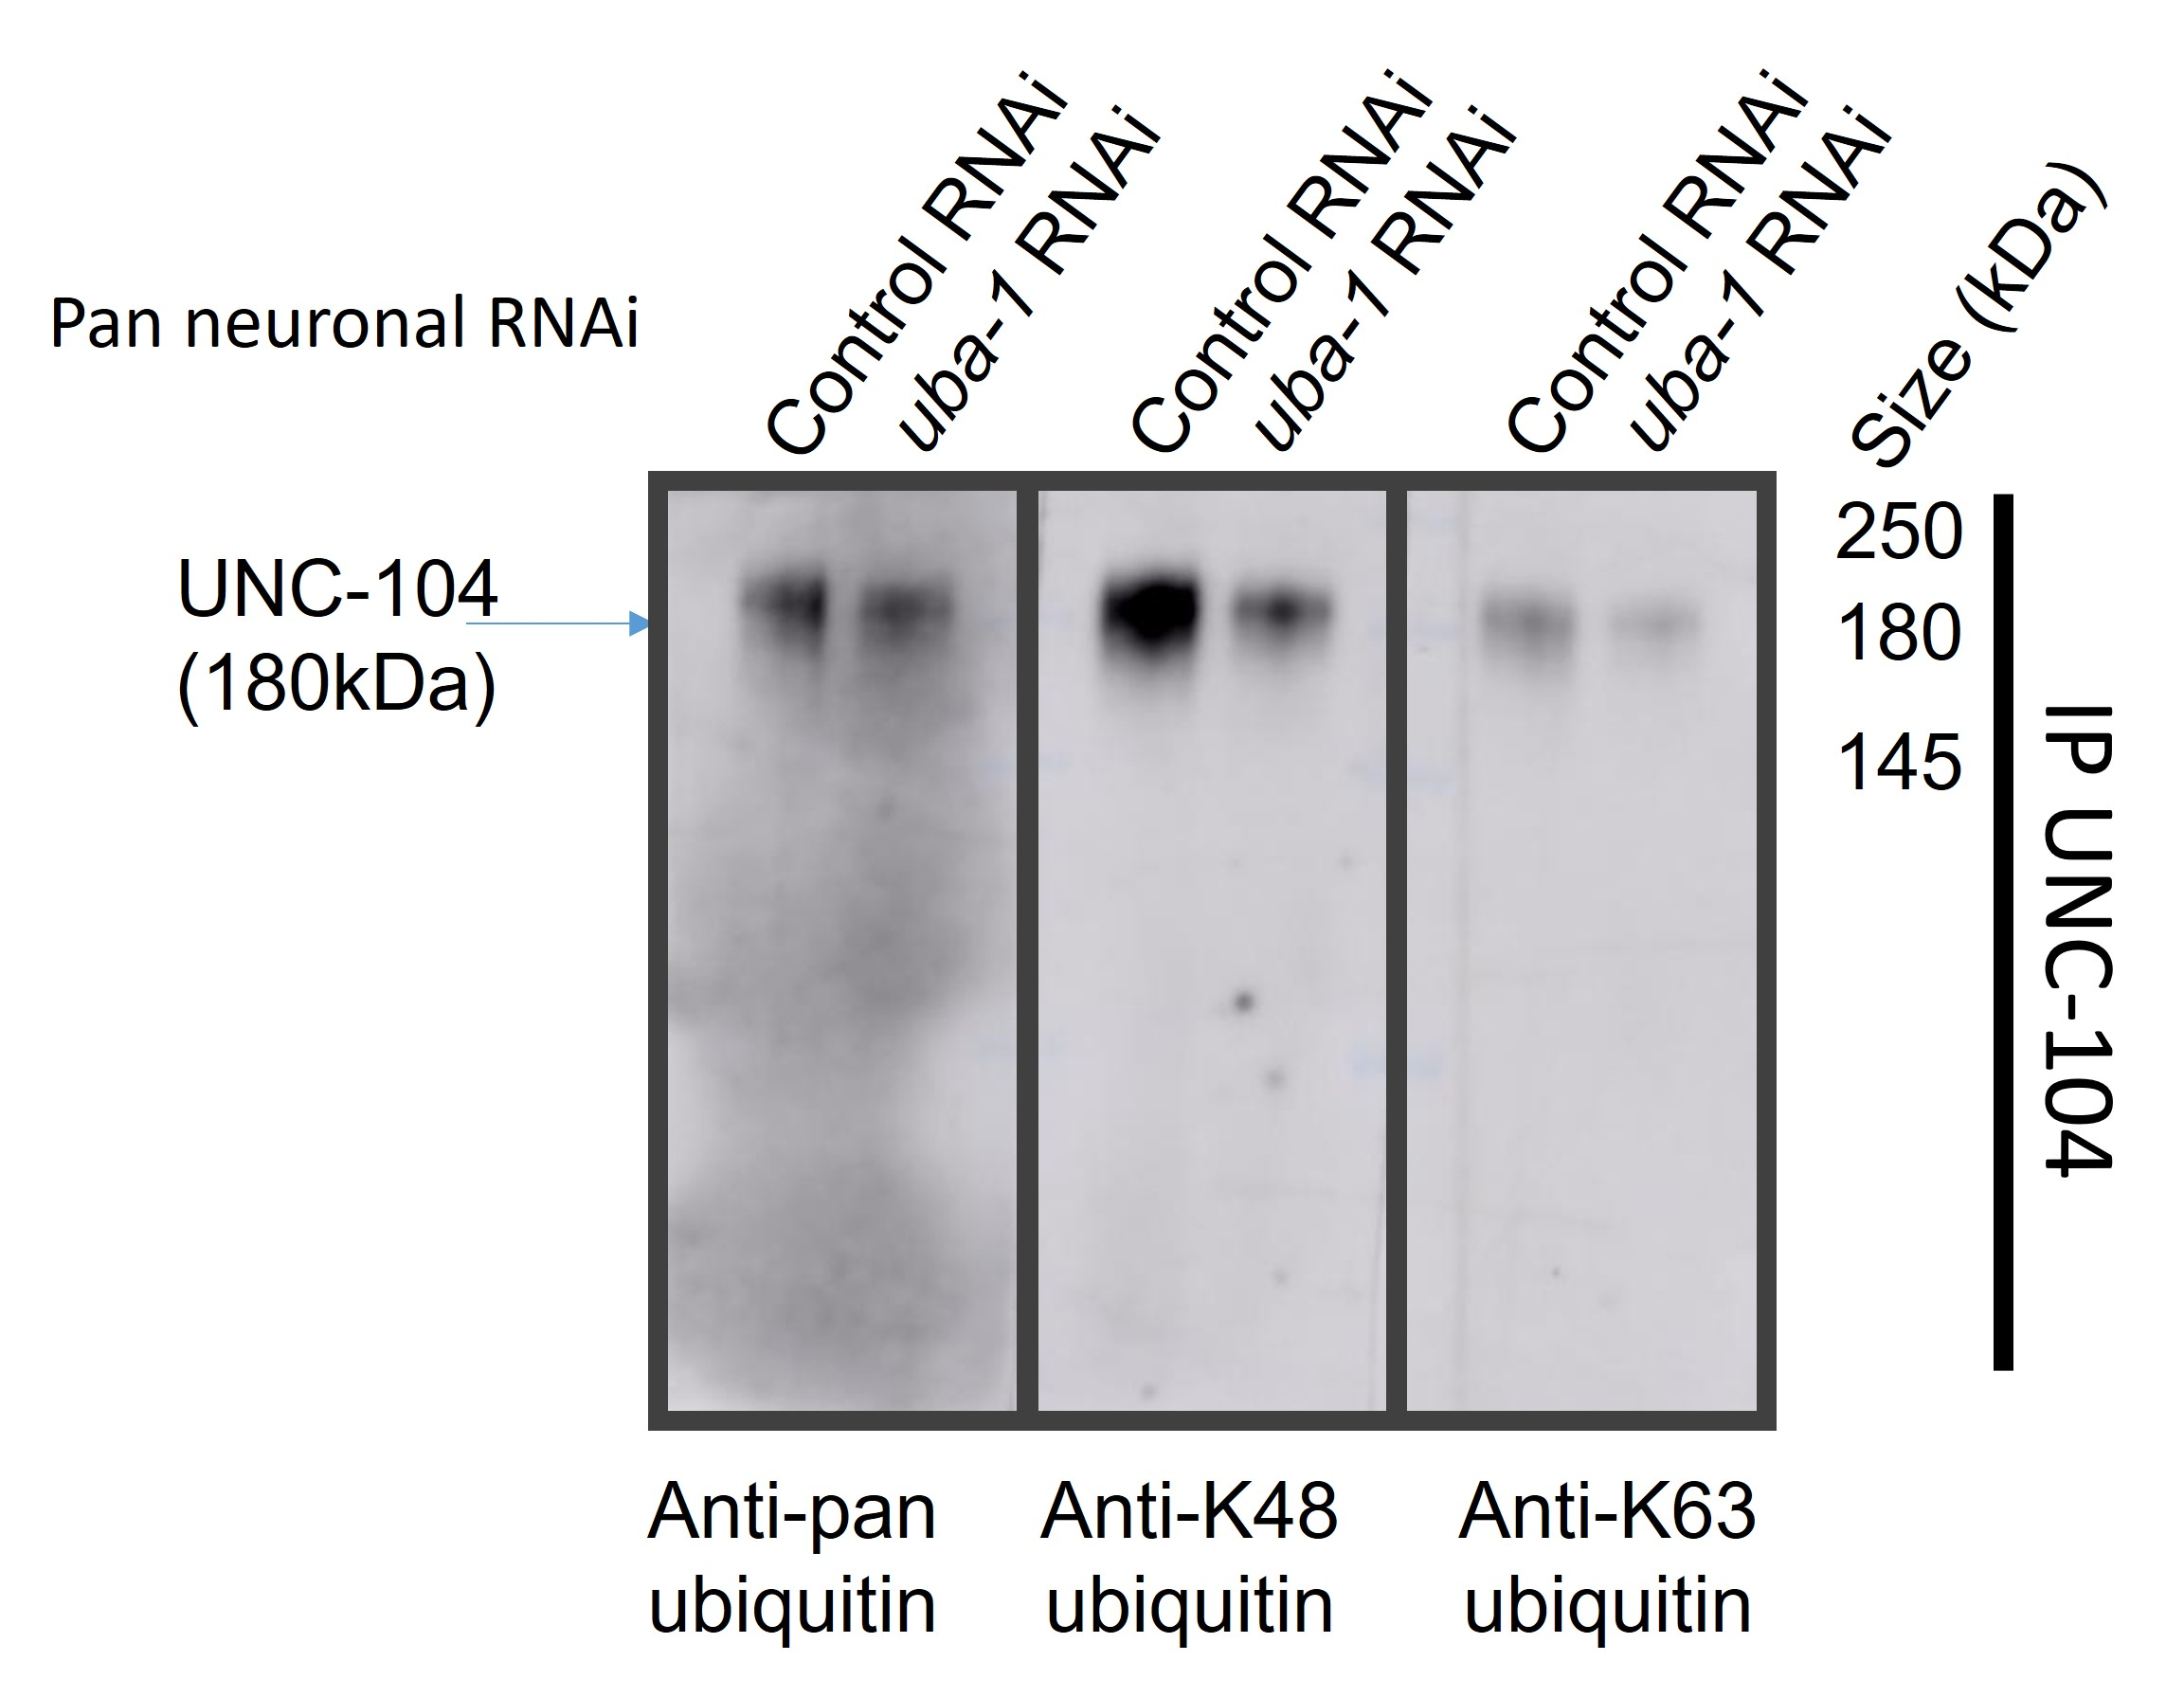
\includegraphics[width=\textwidth]{figs/example}
			
		\end{subfigure}
		\begin{subfigure}{0.3\textwidth}
			\caption{}
			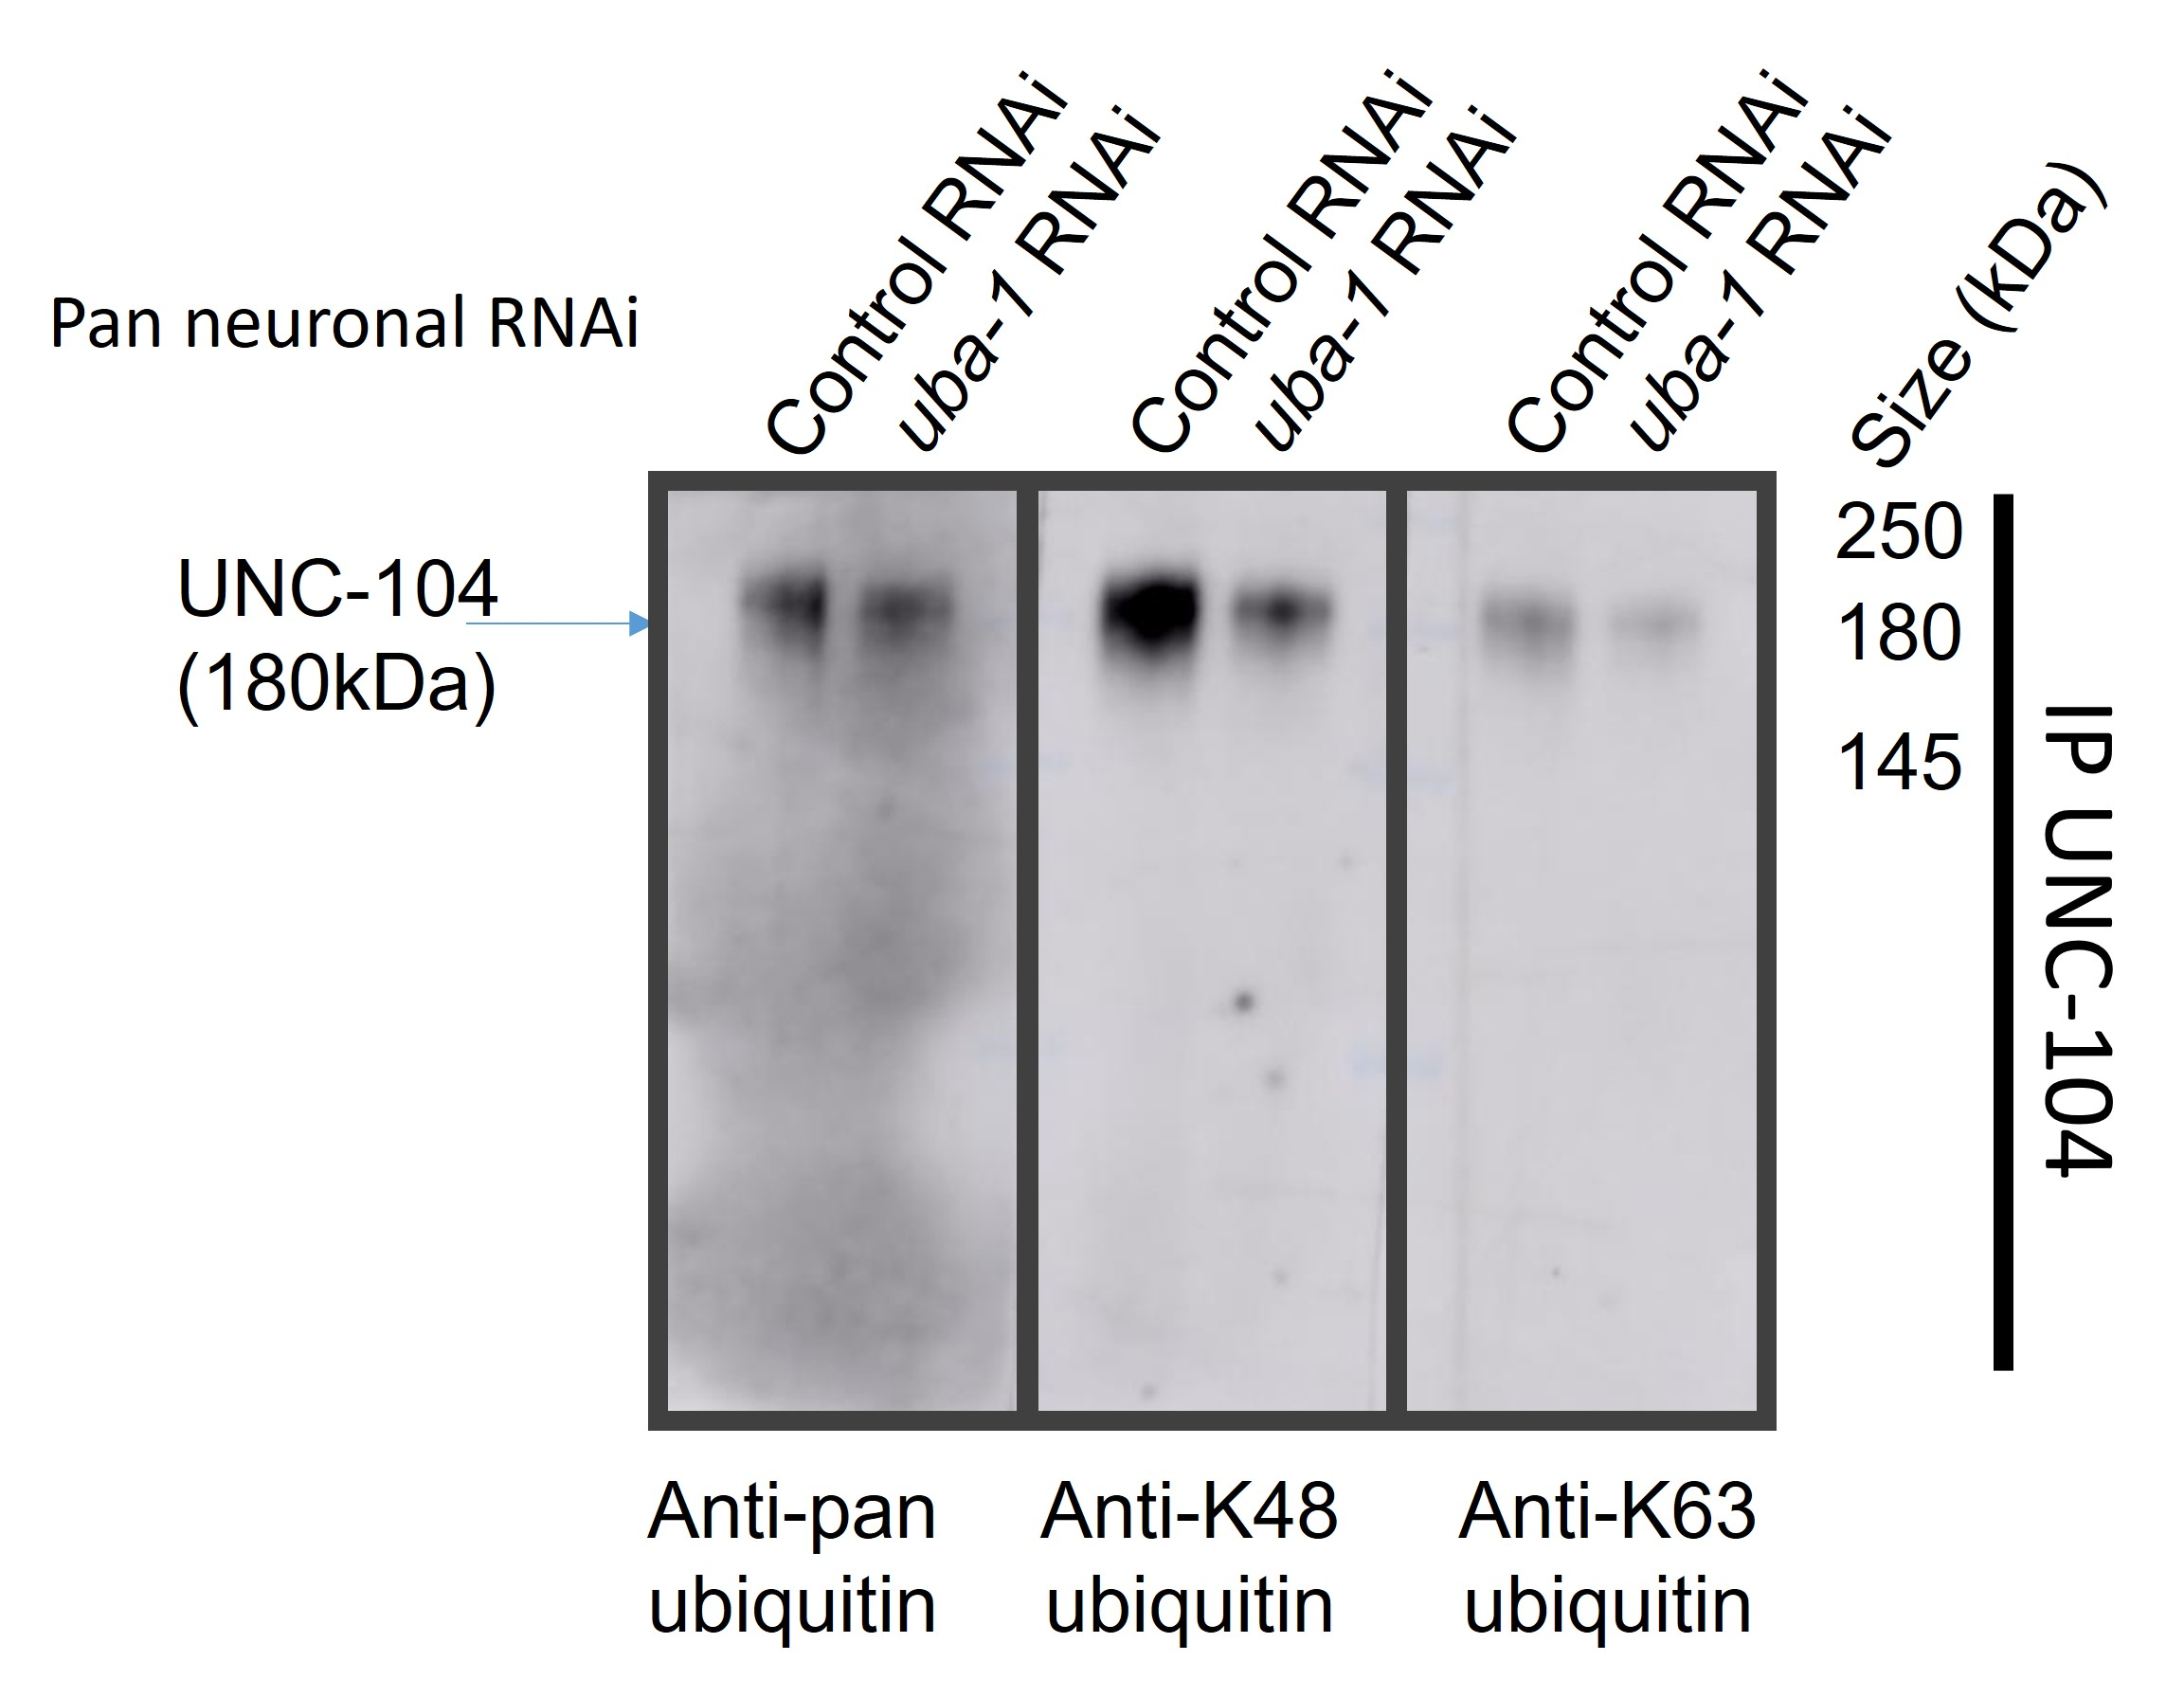
\includegraphics[width=\textwidth]{figs/example}
			
		\end{subfigure}
		
		\caption[Microtubule dynamics start increasing 3 hrs post injury.]{\textbf{Microtubule dynamics start increasing 3 hrs post injury.}} \raggedright \small A) Number of microtubule tracks, B) polymerization velocity, and C) polymerization length of microtubule tracks assessed using EBP-2::GFP comets in the uncut (U), 1 hr post ablation, 2 hrs post ablation, 3 hrs post ablation in wild type. Bar graphs represent the average of at least 15 animals with the whiskers representing S.E.M. One-way ANOVA was used for statistical analysis with all comparisons made with the uncut data for each genotype. **p$<$0.01, ***p$<$0.001.
		\label{fig:MTdyntime}
	\end{figure}
	
	 \subsection{Microtubule dynamics in \textit{dlk-1} and \textit{unc-16} mutants}
	 
	 Previous studies have identified the local upregulation of microtubule dynamics near an injury side in the proximal neuronal process to be important for neuronal outgrowth post injury \parencite{ghosh-roy2012}. We observed that \textit{unc-16(lf)} mutants led to a significant enhancement in the initiation of outgrowth as well as the speed of outgrowth of the neuronal process post injury. To assess if this enhancement is in part due to increased microtubule dynamics, we imaged EBP-2::GFP and characterized the number, polymerization velocity and growth length of these EBP-2::GFP labeled trails. We observed that the baseline number of trails were significantly increased in \textit{unc-16(lf)} mutants compared to wild type, and these numbers were significantly enhanced post injury by a similar fraction as that in wild type [Fig.~\ref{fig:MTdynmut}A]. There was a small insignificant increase in polymerization speed of the EBP-2::GFP trails, along with a significant increase in the growth length in both wild type and \textit{unc-16(lf)} [Fig.~\ref{fig:MTdynmut}A]. To see if these enhanced microtubule dynamics relied on the necessary MAPKKK protein, DLK-1, we built doubles of \textit{unc-16(lf)} with either \textit{dlk-1(null)} or with a rescuing single copy insertion of the growth promoting isoform of DLK, DLK-1L. While the baseline number of EBP-2::GFP trails remain high in the double \textit{dlk-1(null)}; \textit{unc-16(lf)} compared to wild type, there is a drastic reduction in the fractional enhancement EBP-2::GFP tracks post injury along with the length to which EBP-2::GFP polymerizes [Fig.~\ref{fig:MTdynmut}A,C]. The fractional increase in EBP-2::GFP tracks along with the growth length are rescued in a triple strain expressing the growth promoting DLK-1L (Mi(L)) isoform along with the double \textit{dlk-1(null)}; \textit{unc-16(lf)} [Fig.~\ref{fig:MTdynmut}A,C]. Overexpression of UNC-16 using a pan-neuronal promoter led to an increase in the baseline microtubule dynamics, but did not alter the fractionaly increase in number of EBP-2::GFP trails post injury [Fig.~\ref{fig:MTdynmut}A]. The polarity of microtubules were not dependent on any of these mutants and a slight deviation from unipolar microtubules were observed 6 hrs post injury, only near the cut site [Fig.~\ref{fig:MTdynmut}D].
	
	DLK-1 may signal to the nucleus via the transcription factor CEBP-1, or may influence protein activity locally near the cut site, such as by increasing activity of kinesin-13	member KLP-7's microtubule severing activity or via microtubule modification via the cytosolic carboxypeptidase, CCPP-6. Thus, we tested if \textit{unc-16(lf)} acts through signaling to the nucleus to upregulate microtubule dynamics near the cut site by building doubles with the \textit{cebp-1(lf)} mutant. While \textit{cebp-1(lf)} indeed has lower number of EBP-2::GFP trails compared to wild type, there is still a slight non-significant increase in the number of trails post injury and the growth length of the microtubules [Fig.~\ref{fig:MTdyncebp}A,B,C]. The double \textit{unc-16(lf)}; \textit{cebp-1(lf)} looks largely like the single
	\begin{figure}[H]
%		\centering
	\begin{minipage}[t]{0.65\textwidth}
		\vspace{0pt}
		%	\hfill
		\begin{subfigure}{1\textwidth}
			\caption{}
			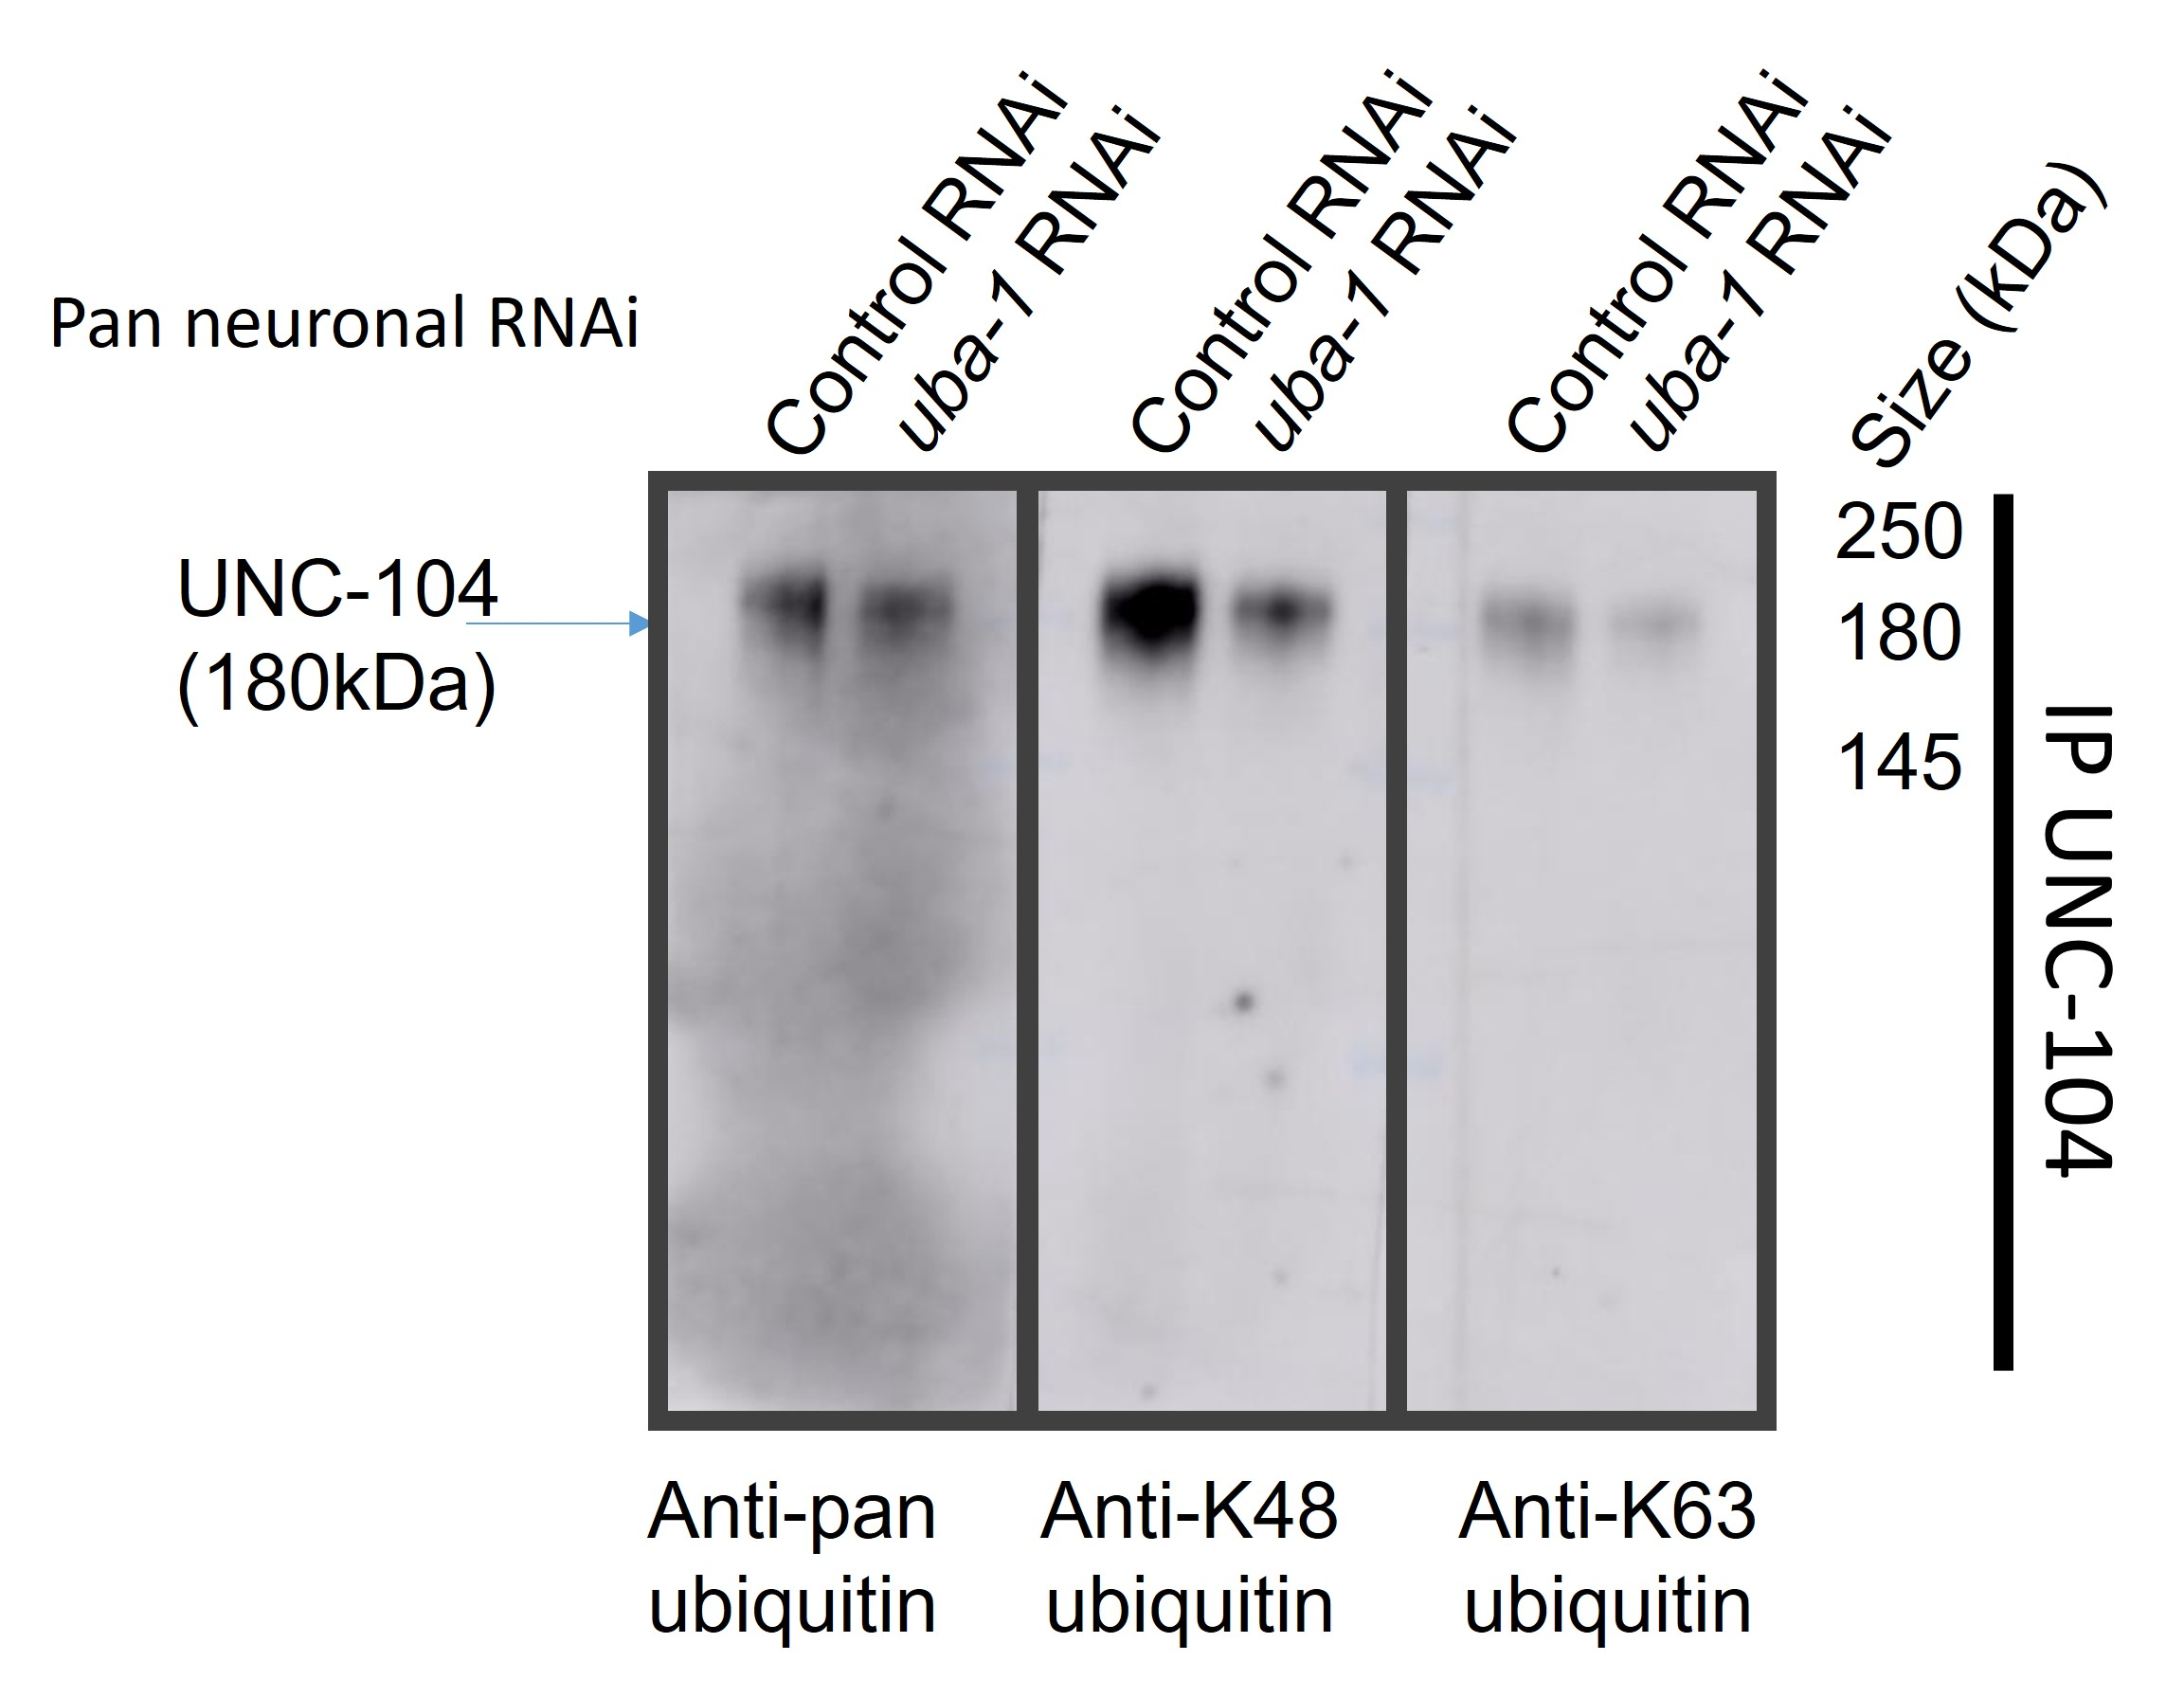
\includegraphics[width=\textwidth]{figs/example}
			
		\end{subfigure}
		\begin{subfigure}{1\textwidth}
			\caption{}
			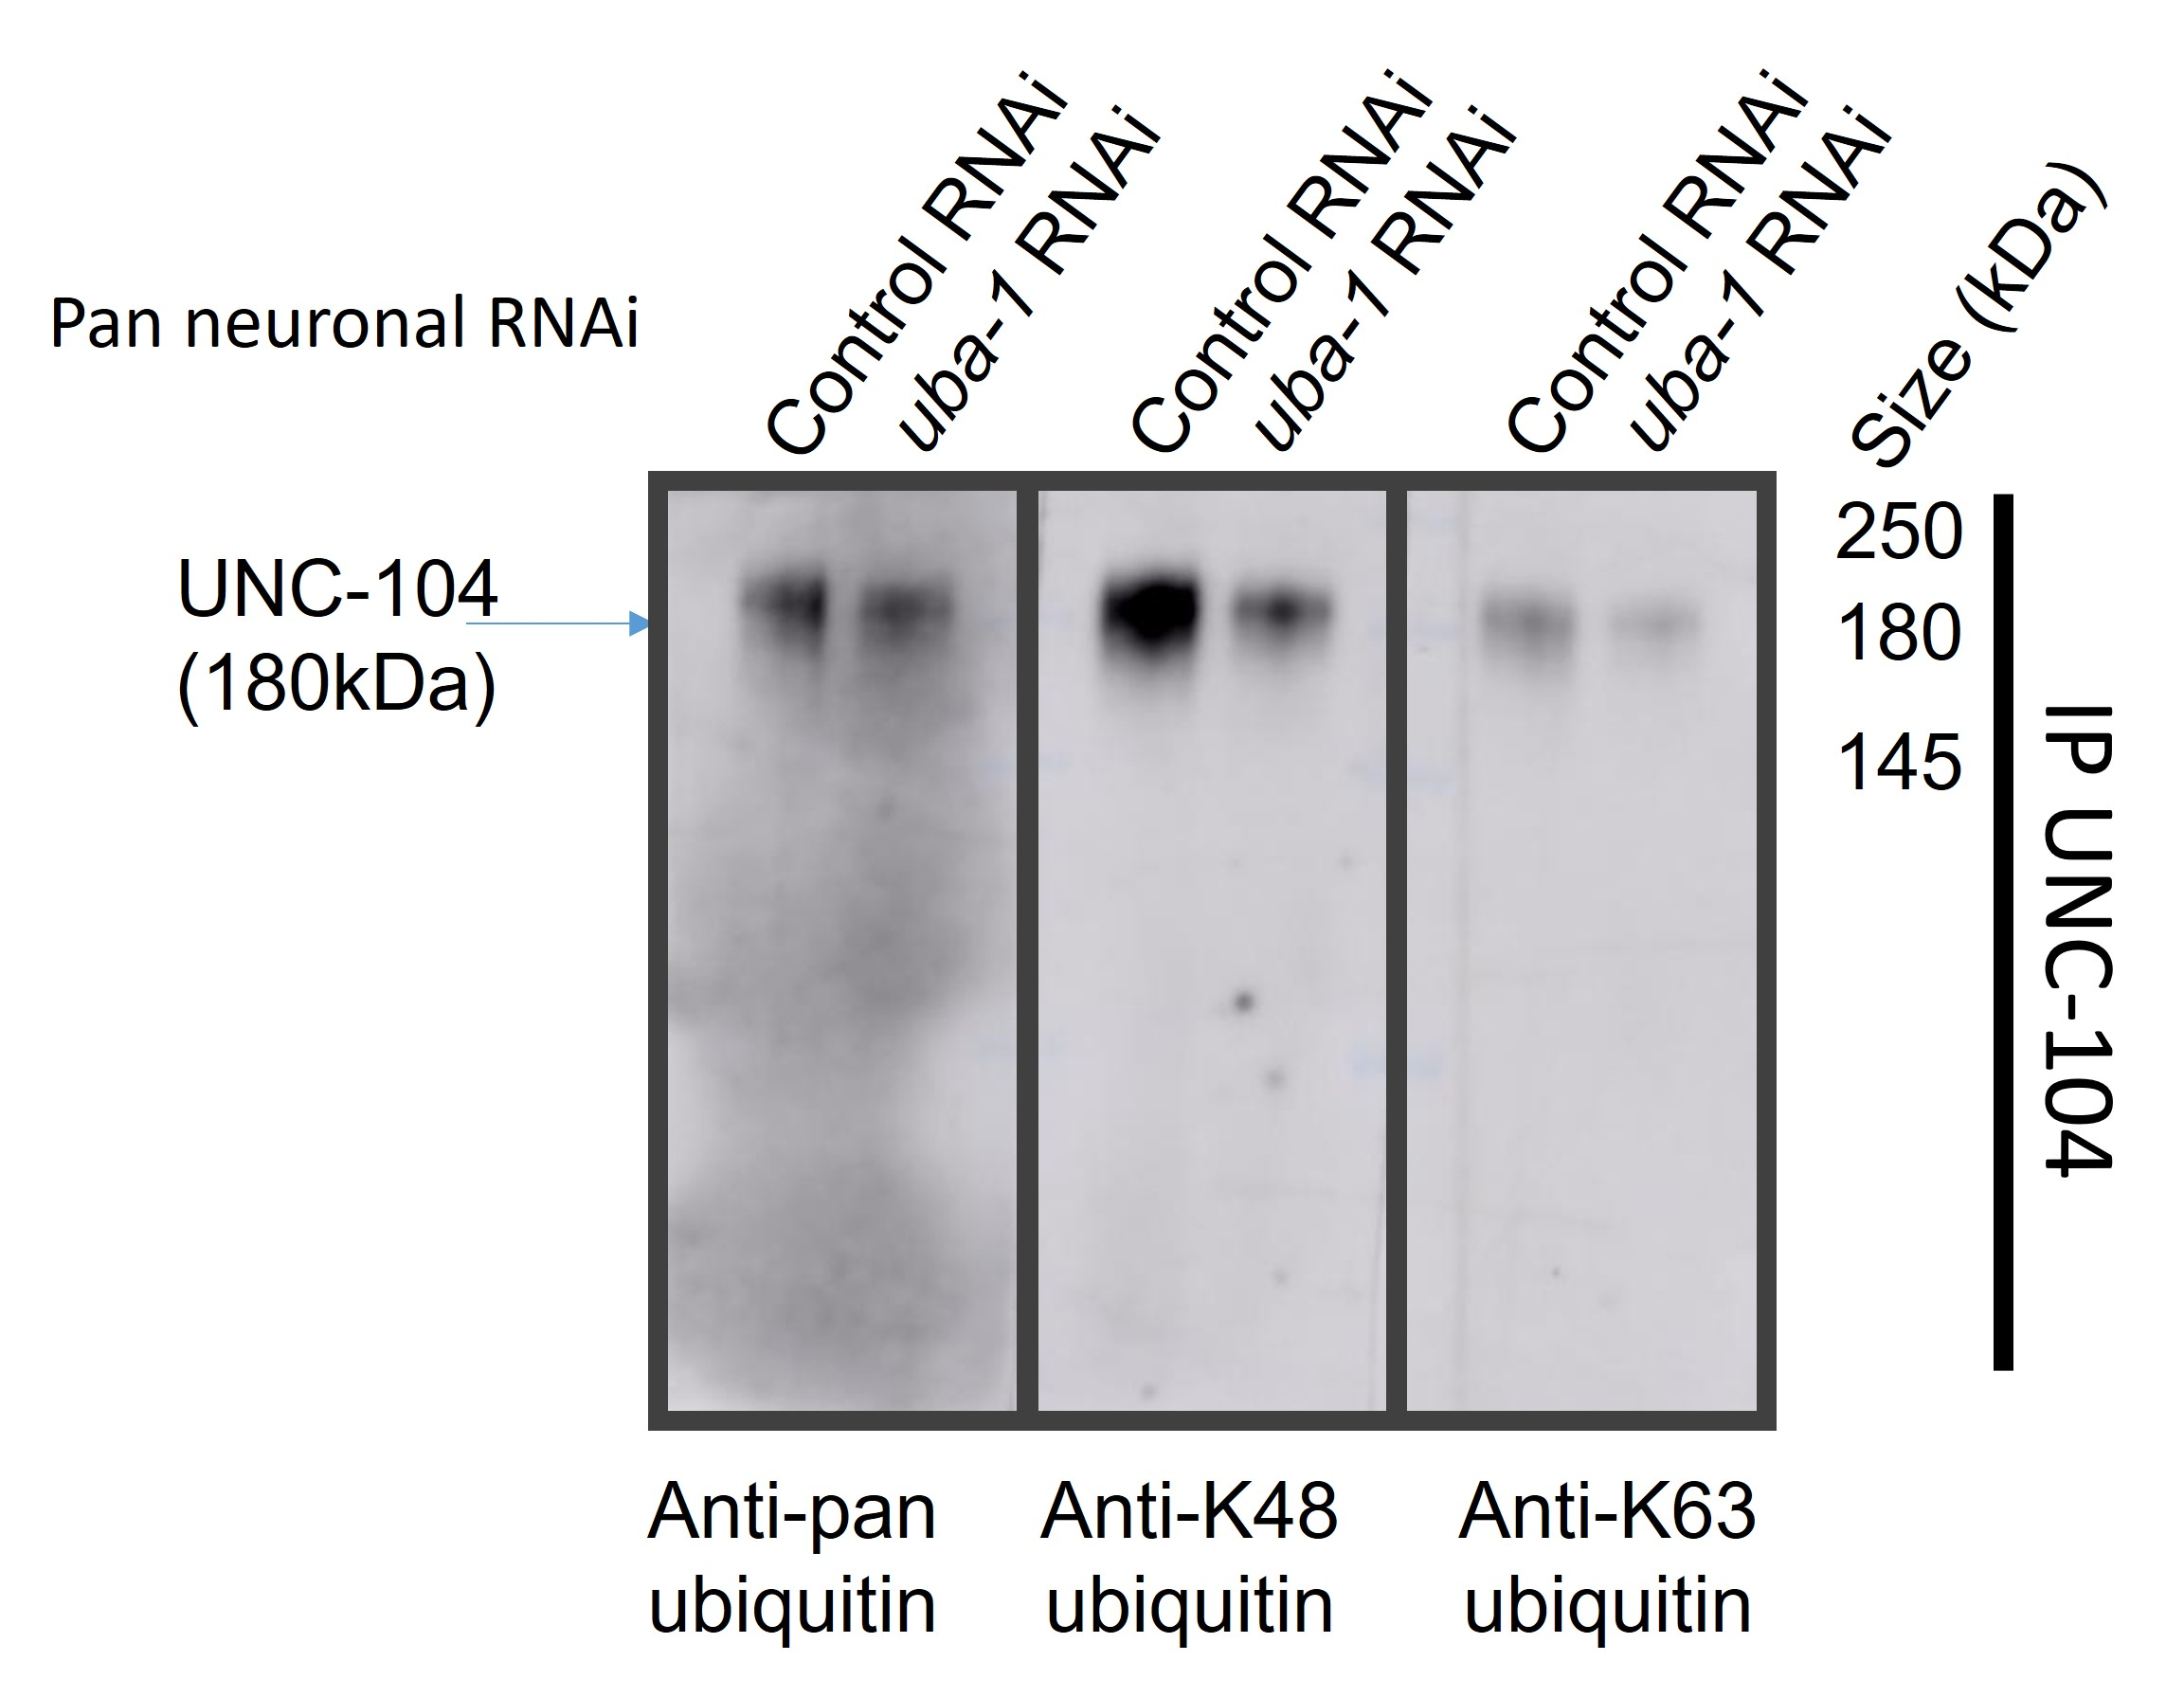
\includegraphics[width=\textwidth]{figs/example}
			
		\end{subfigure}
		\begin{subfigure}{1\textwidth}
			\caption{}
			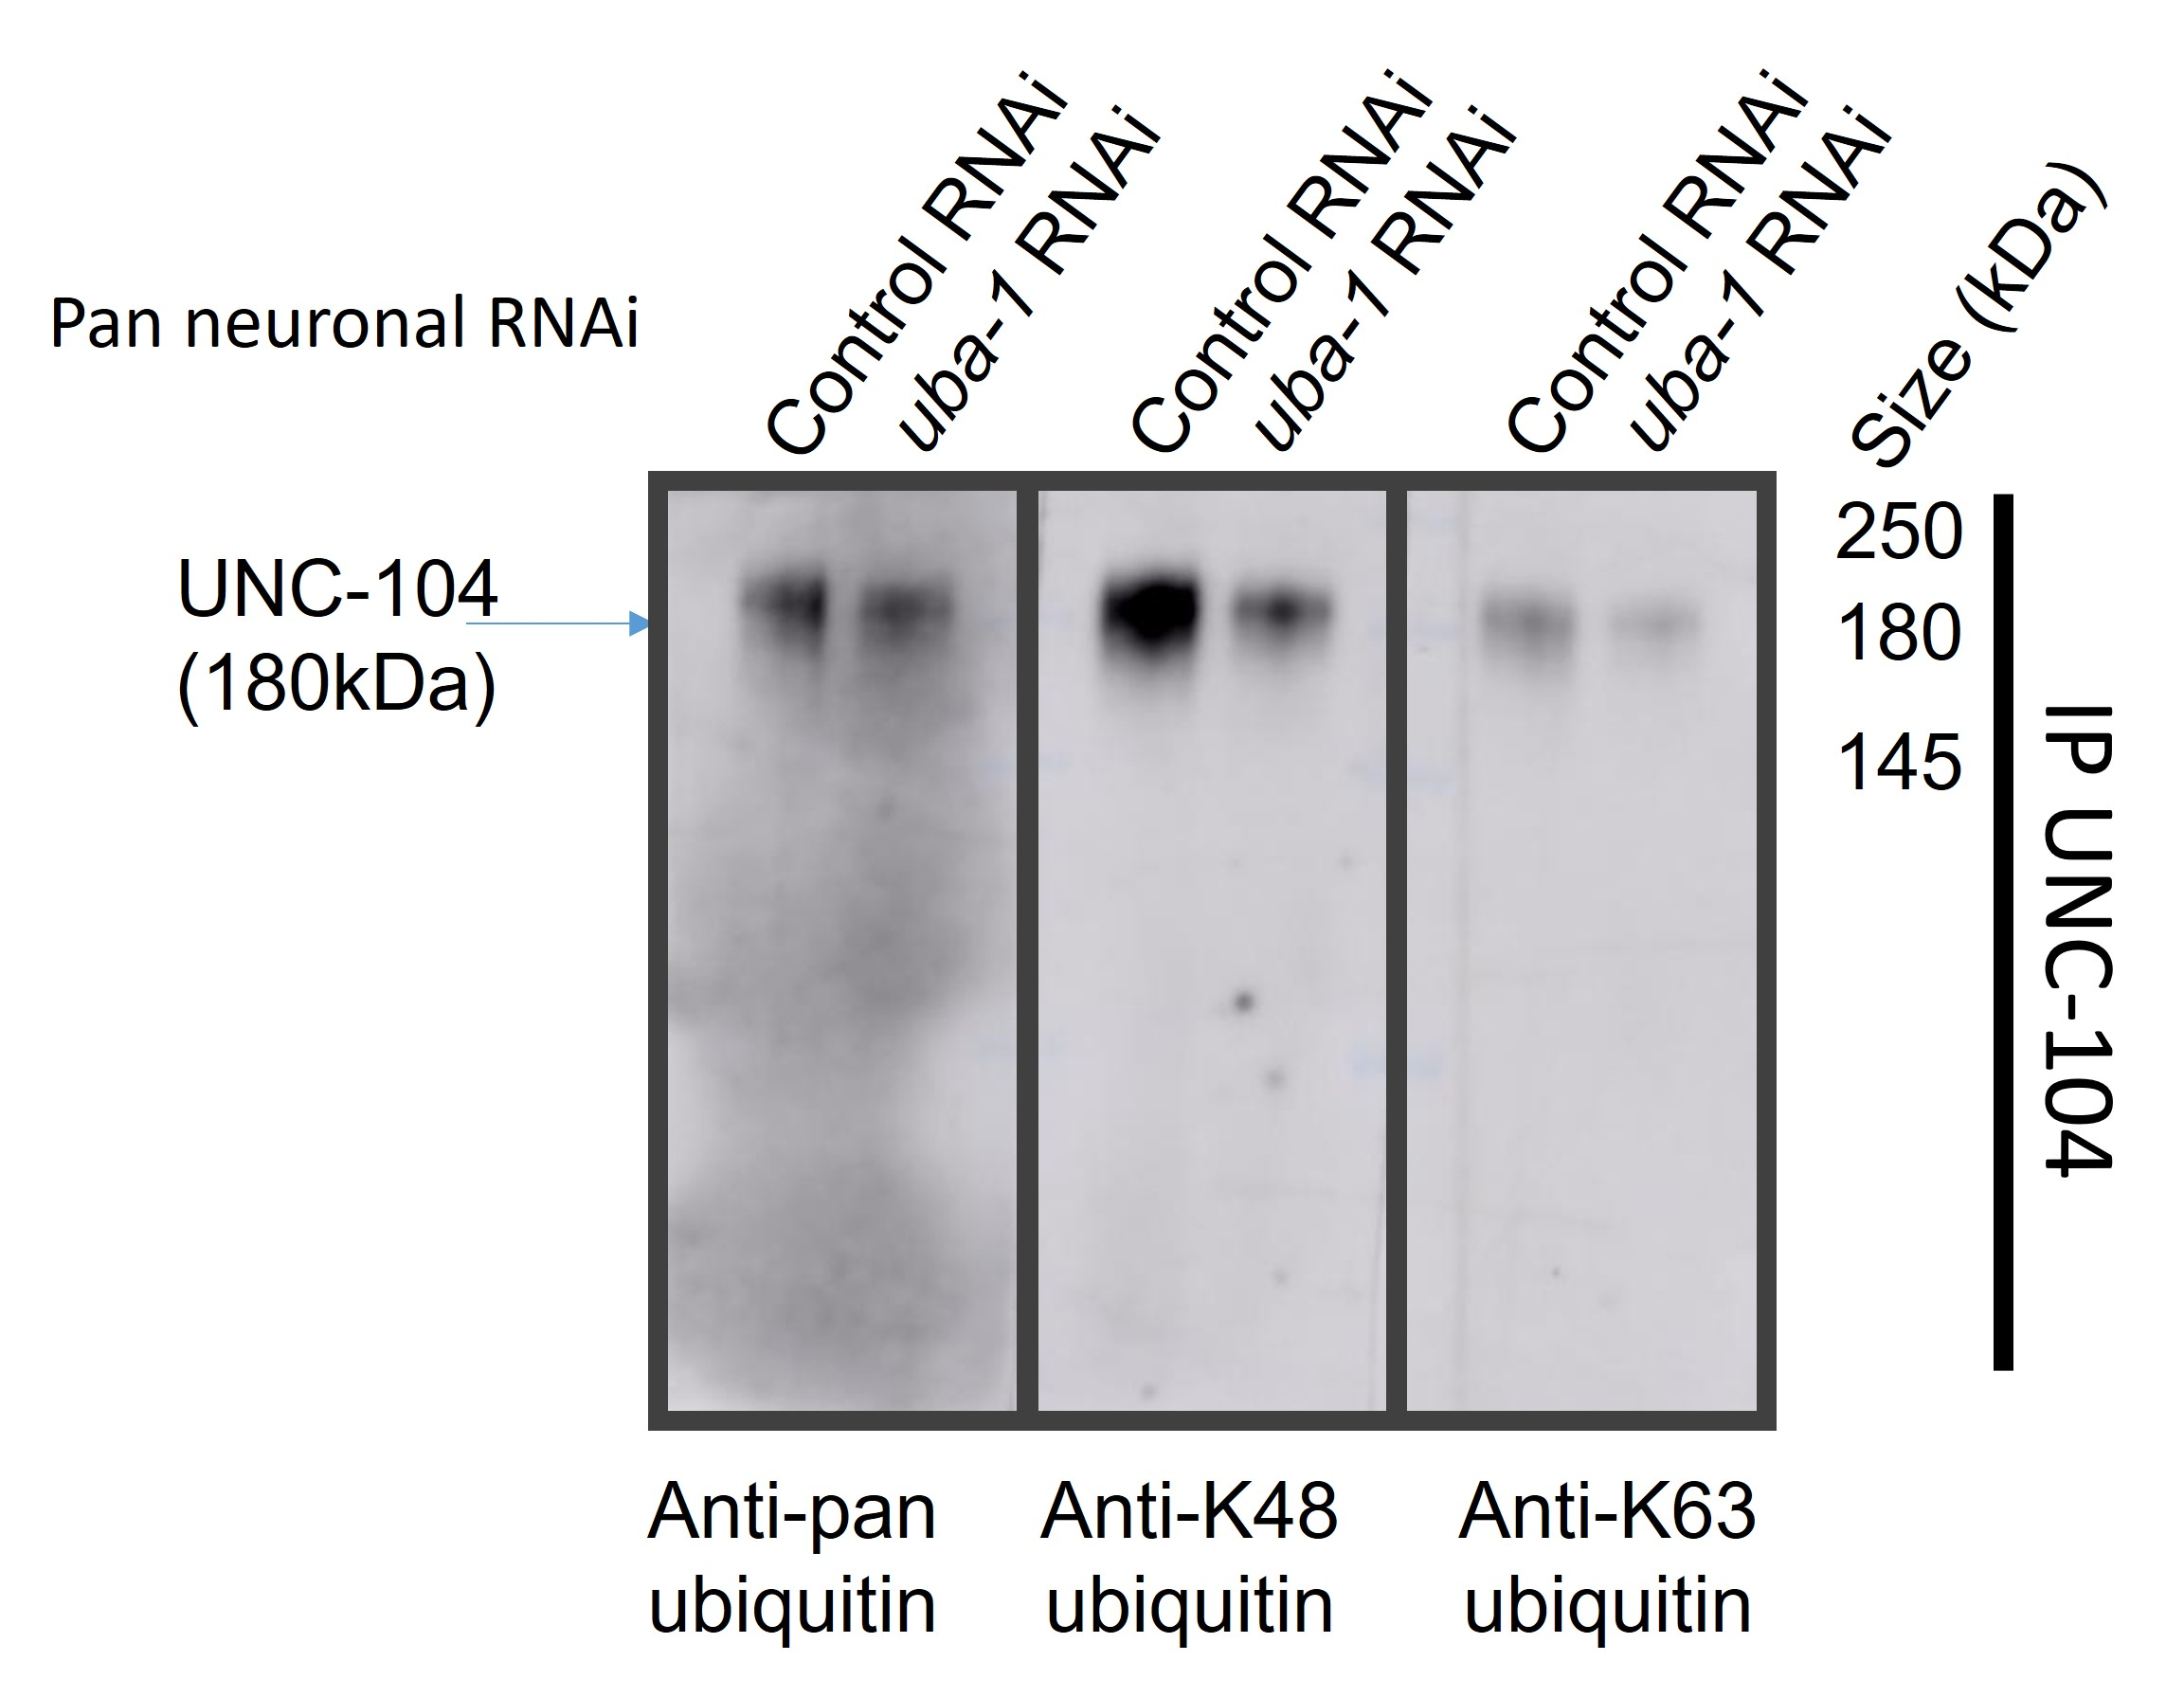
\includegraphics[width=\textwidth]{figs/example}
			
		\end{subfigure}
		\begin{subfigure}{1\textwidth}
			\caption{}
			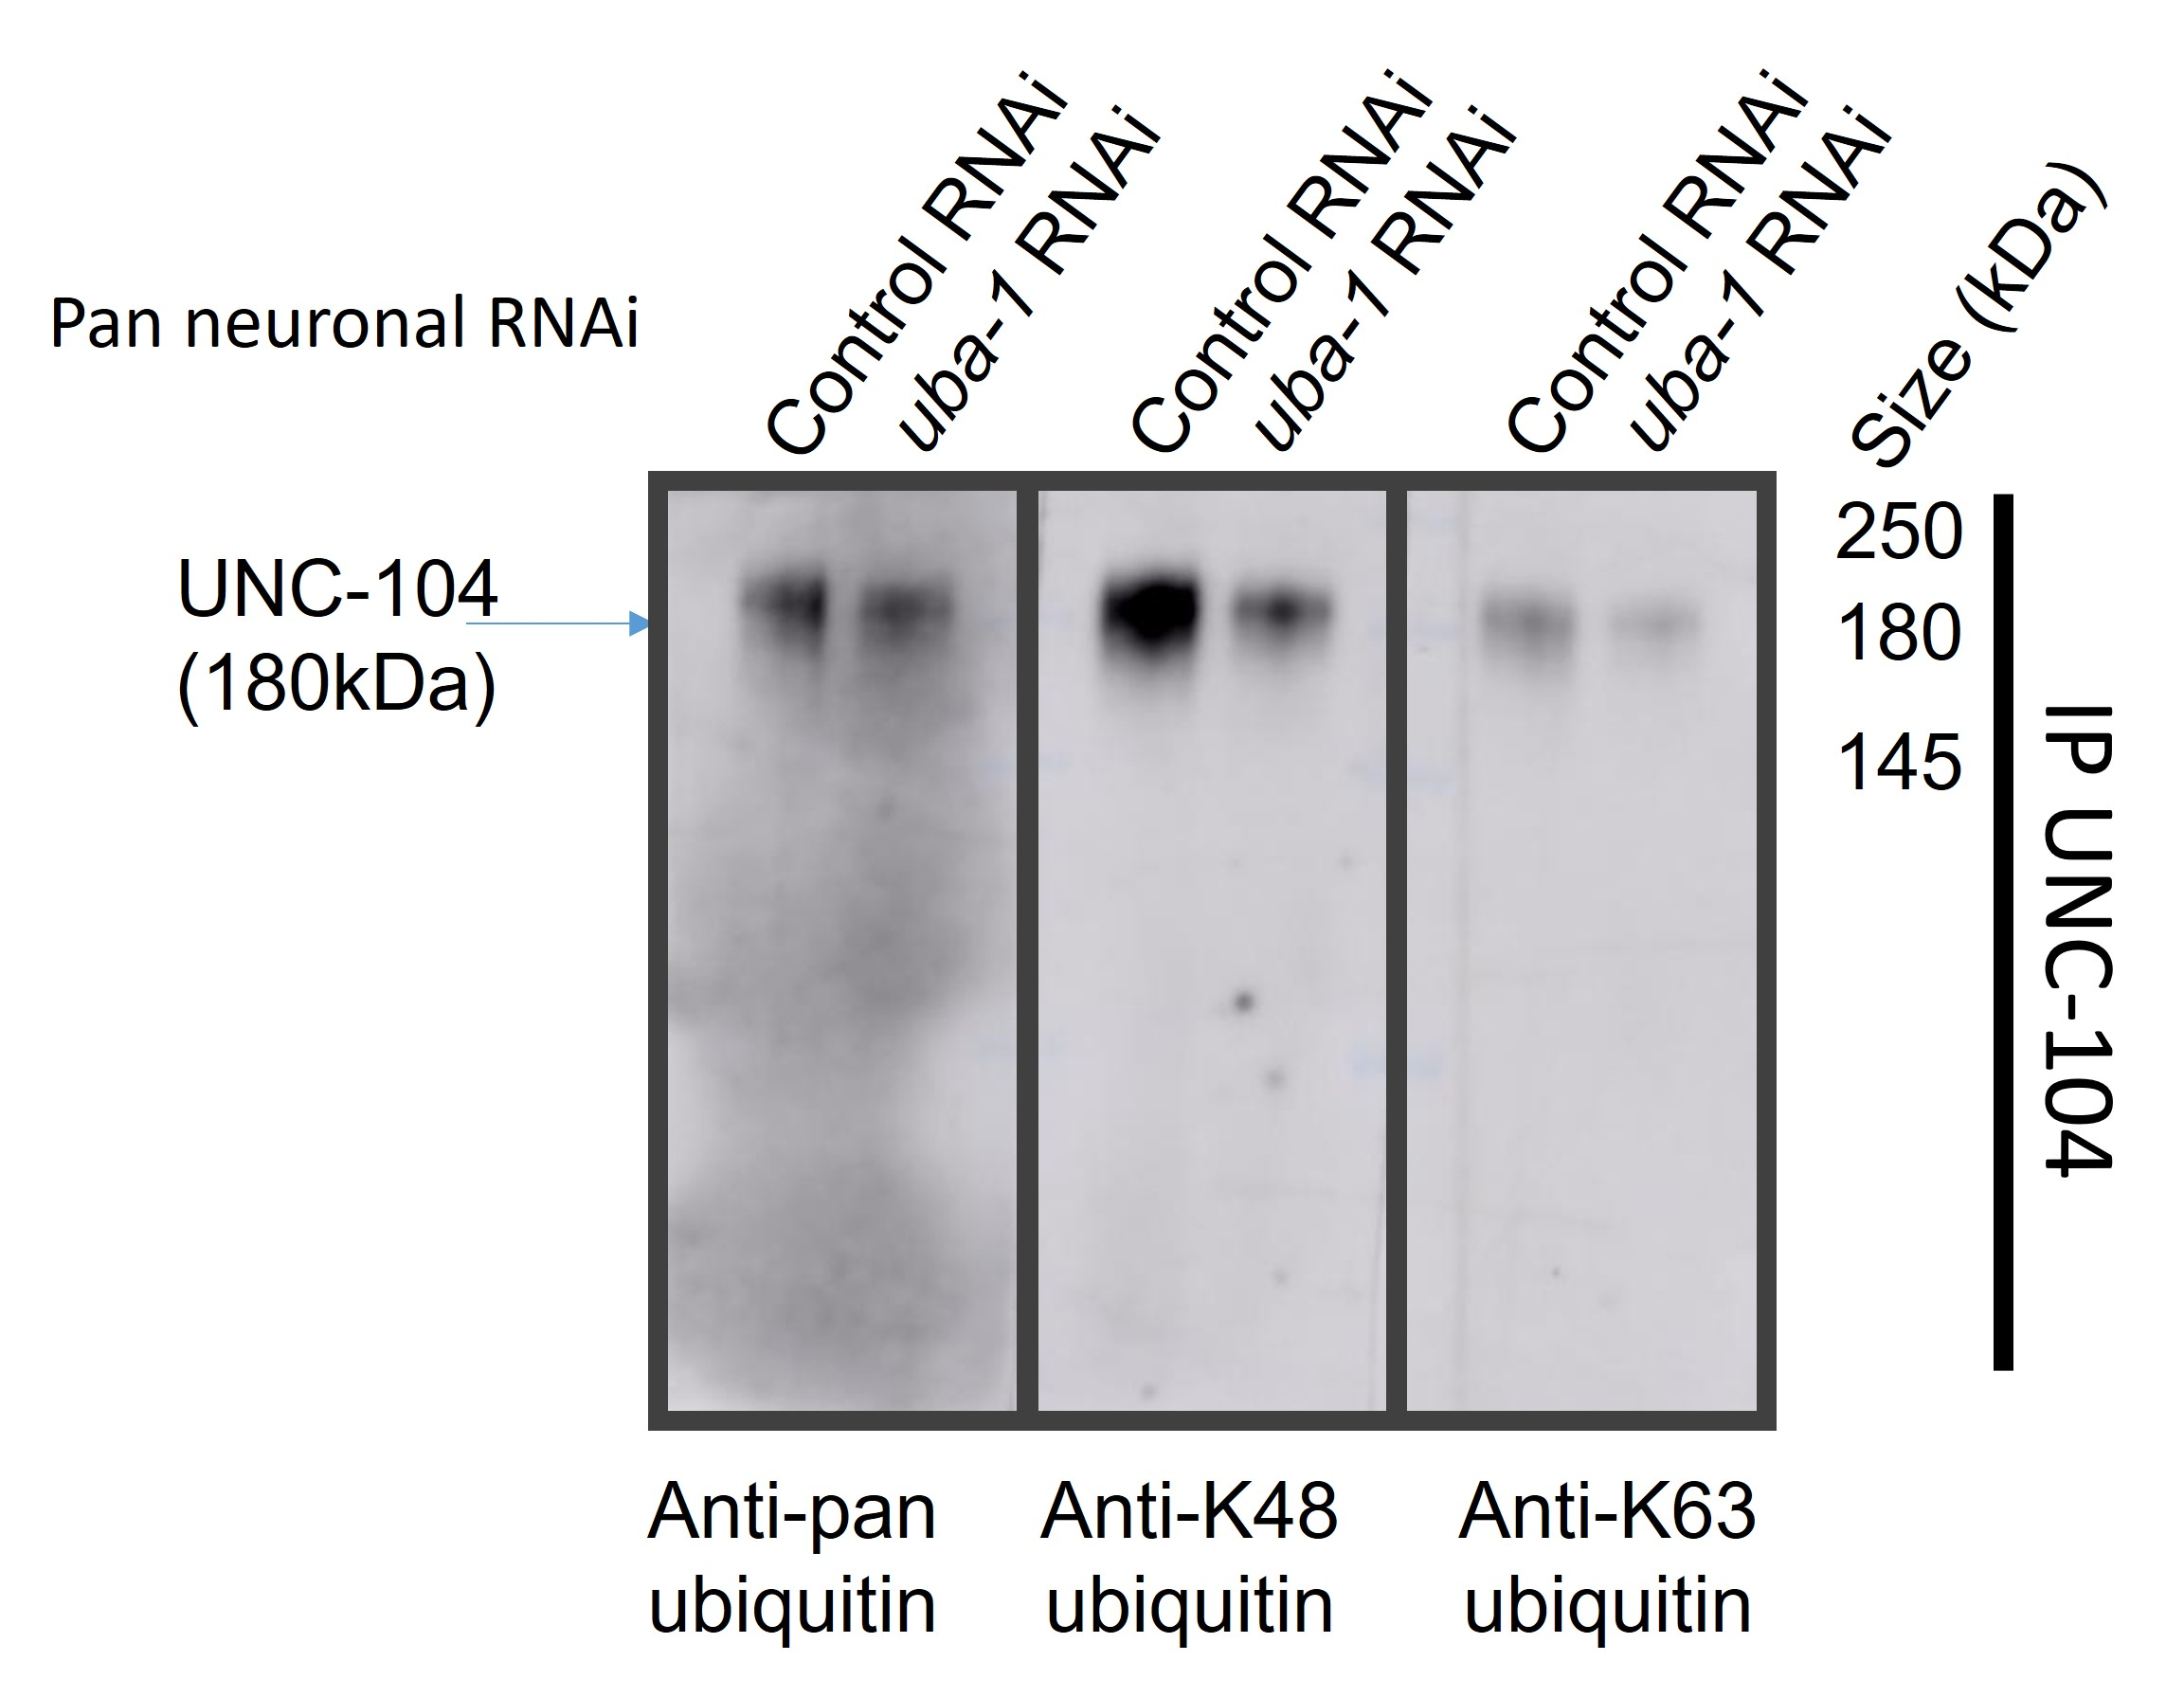
\includegraphics[width=\textwidth]{figs/example}
			
		\end{subfigure}
		
	\end{minipage}
	\begin{minipage}[t]{0.3\textwidth}
		\vspace{0pt}
		\caption[Increase in microtubule dynamics post ablation is enhanced in \textit{unc-16(lf)}.]{\textbf{Increase in microtubule dynamics post ablation is enhanced in \textit{unc-16(lf)}.}} \raggedright \small A) Number of microtubule tracks, B) polymerization velocity, C) polymerization length, or D) polarity of microtubule tracks assessed using EBP-2::GFP comets in the uncut (U), immediately post ablation (0), 3 hrs post ablation (3), or 6 hrs post ablation (6) in wild type, \textit{dlk-1(null)}, \textit{unc-16(lf)}, DLK-1 long isoform overexpression, UNC-16 overexpression, or their combinations. A,B,C) Bar graphs represent the average of at least 15 animals with the whiskers representing S.E.M. One-way ANOVA was used for statistical analysis with all comparisons made with the 0 hr data for each genotype. *p$<$0.05, **p$<$0.01, ***p$<$0.001. D) Fraction of all EBP-2::GFP comets either in the anterograde (black), or retrograde (gray) directions. All N$>$15.
		\label{fig:MTdynmut}
	\end{minipage}
	\end{figure}

	  \textit{cebp-1(lf)} for the number of EBP-2::GFP trails [Fig.~\ref{fig:MTdyncebp}A], while the double looks like the \textit{unc-16(lf)} single for the EBP-2::GFP growth length [Fig.~\ref{fig:MTdyncebp}C]. Thus, the microtubule growth length and number of dynamic microtubules may be regulated by two different paths, with the enhanced number of dynamic microtubules in \textit{unc-16(lf)} depending on \textit{cebp-1}.
	
	
	\begin{figure}[H]
		\centering
		\begin{subfigure}{0.32\textwidth}
			\caption{}
			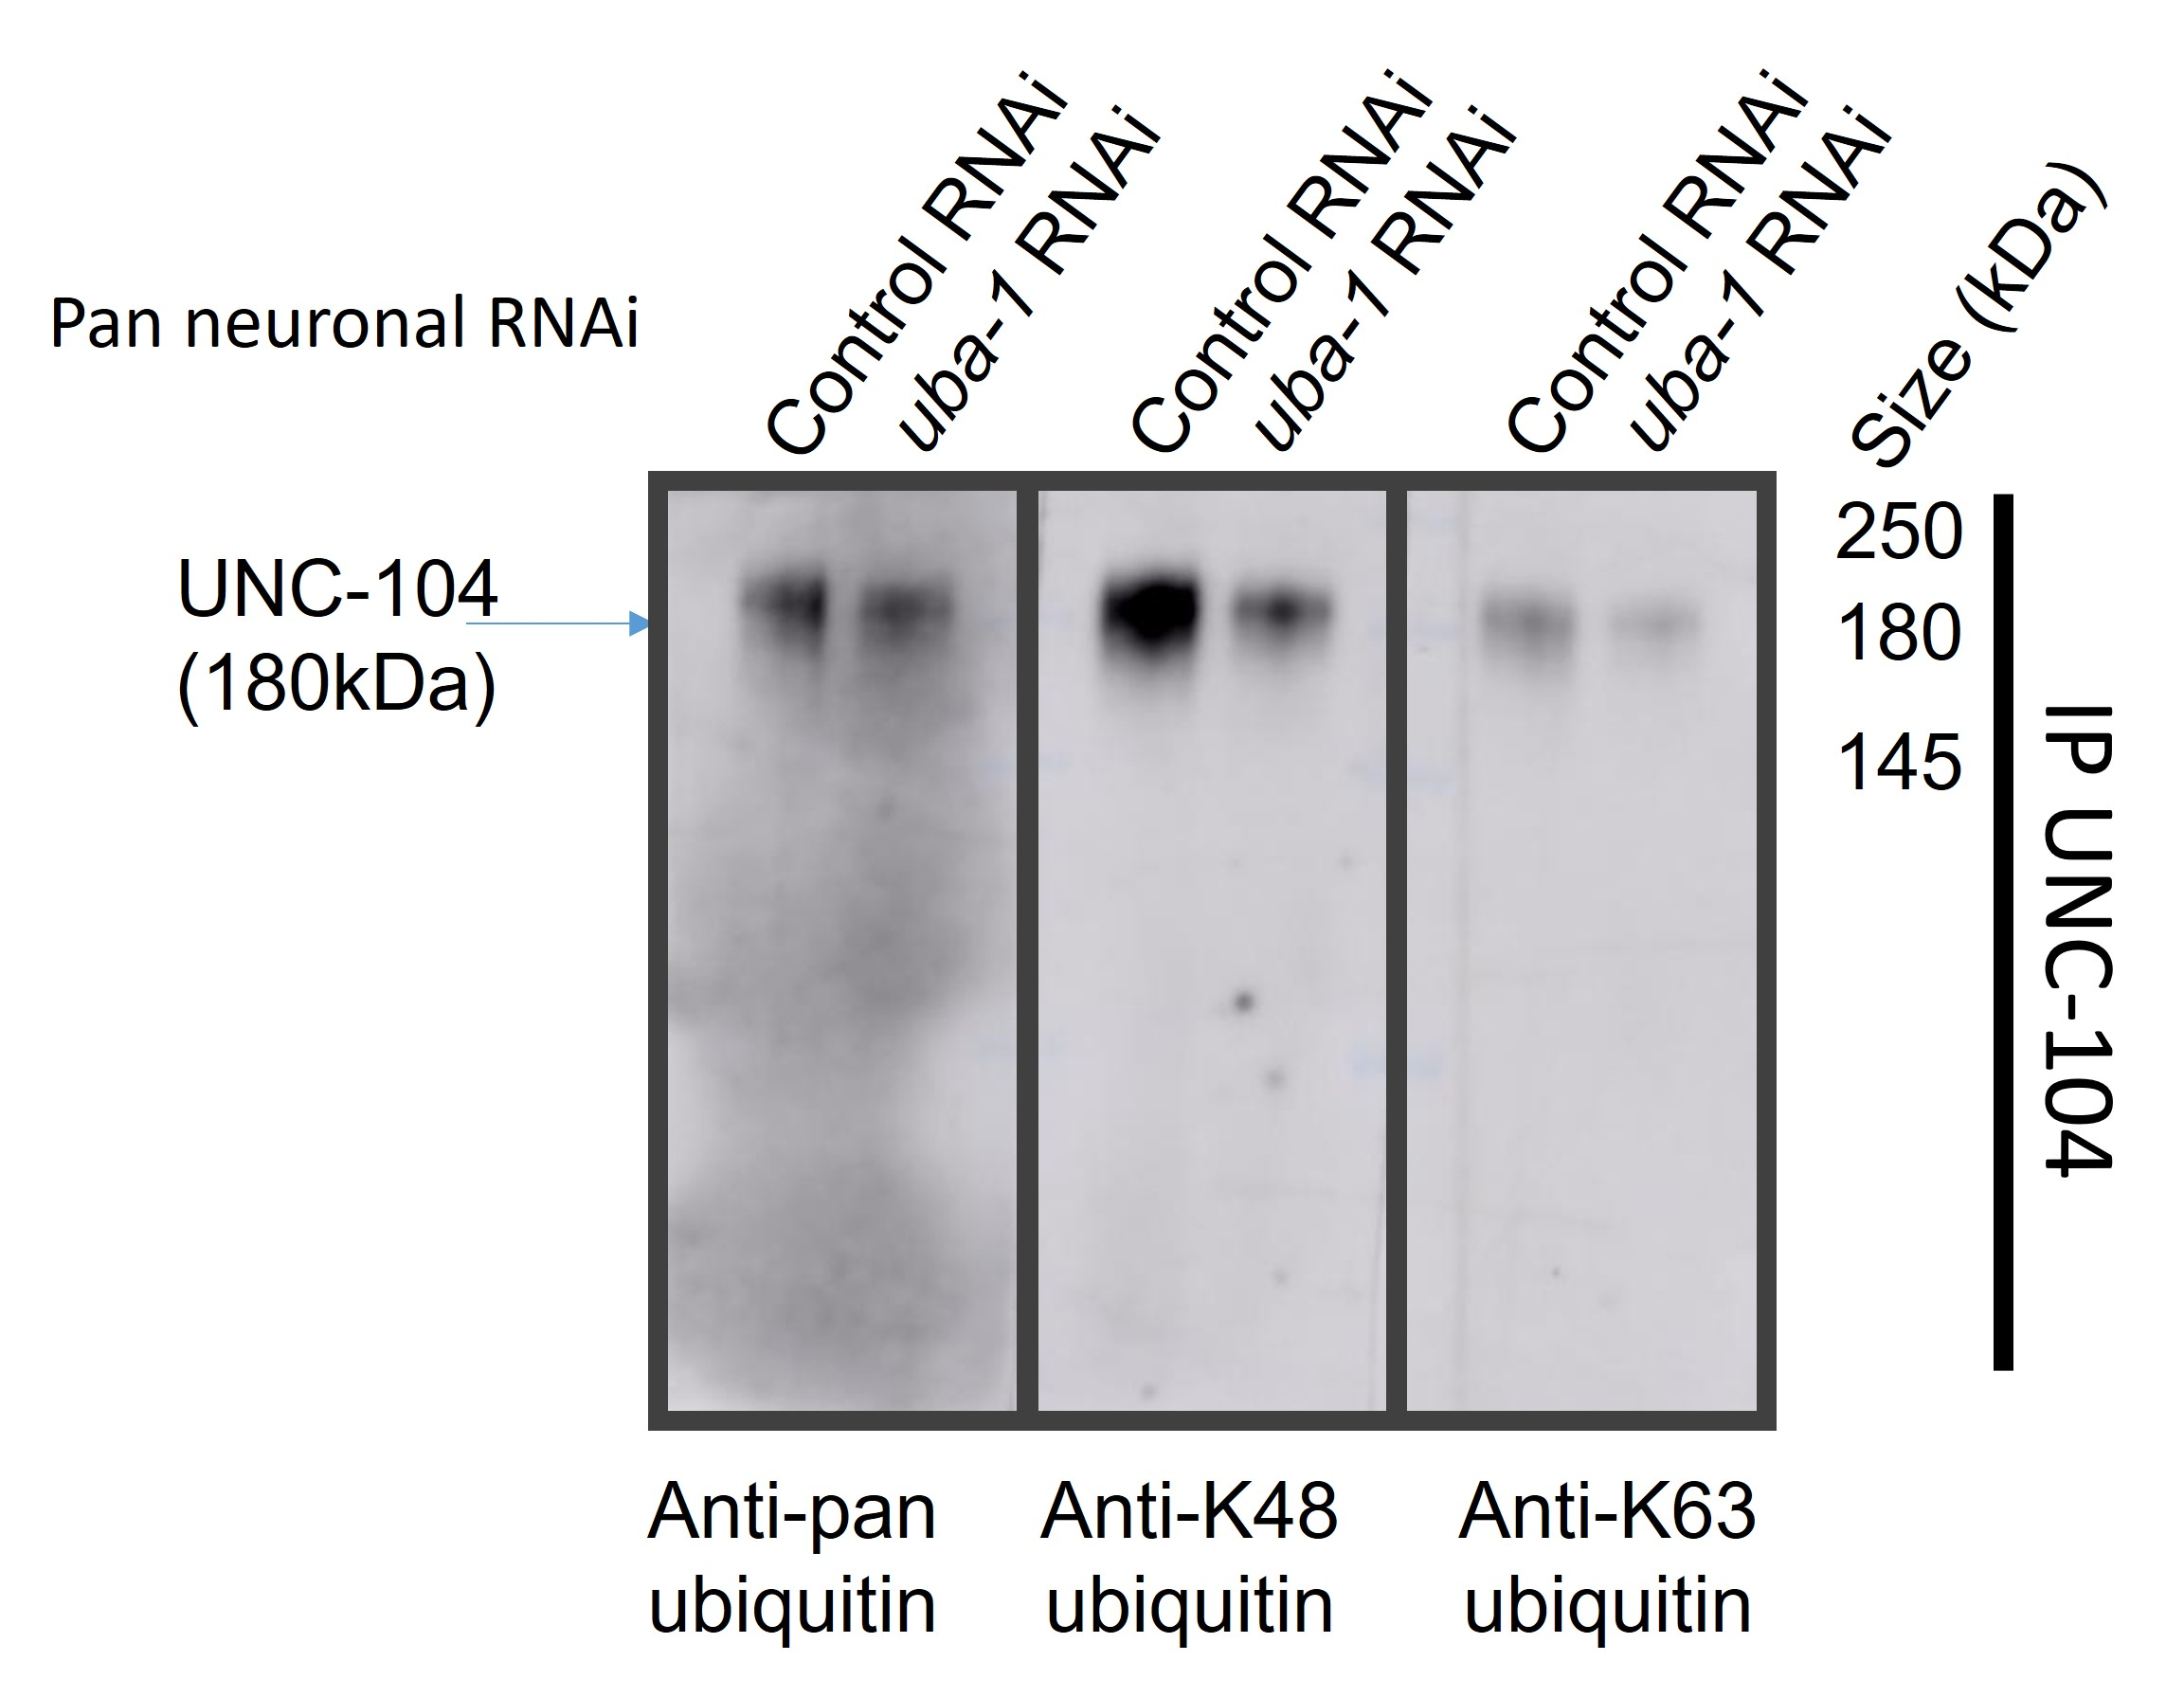
\includegraphics[width=\textwidth]{figs/example}
			
		\end{subfigure}
		%	\hfill
		\begin{subfigure}{0.32\textwidth}
			\caption{}
			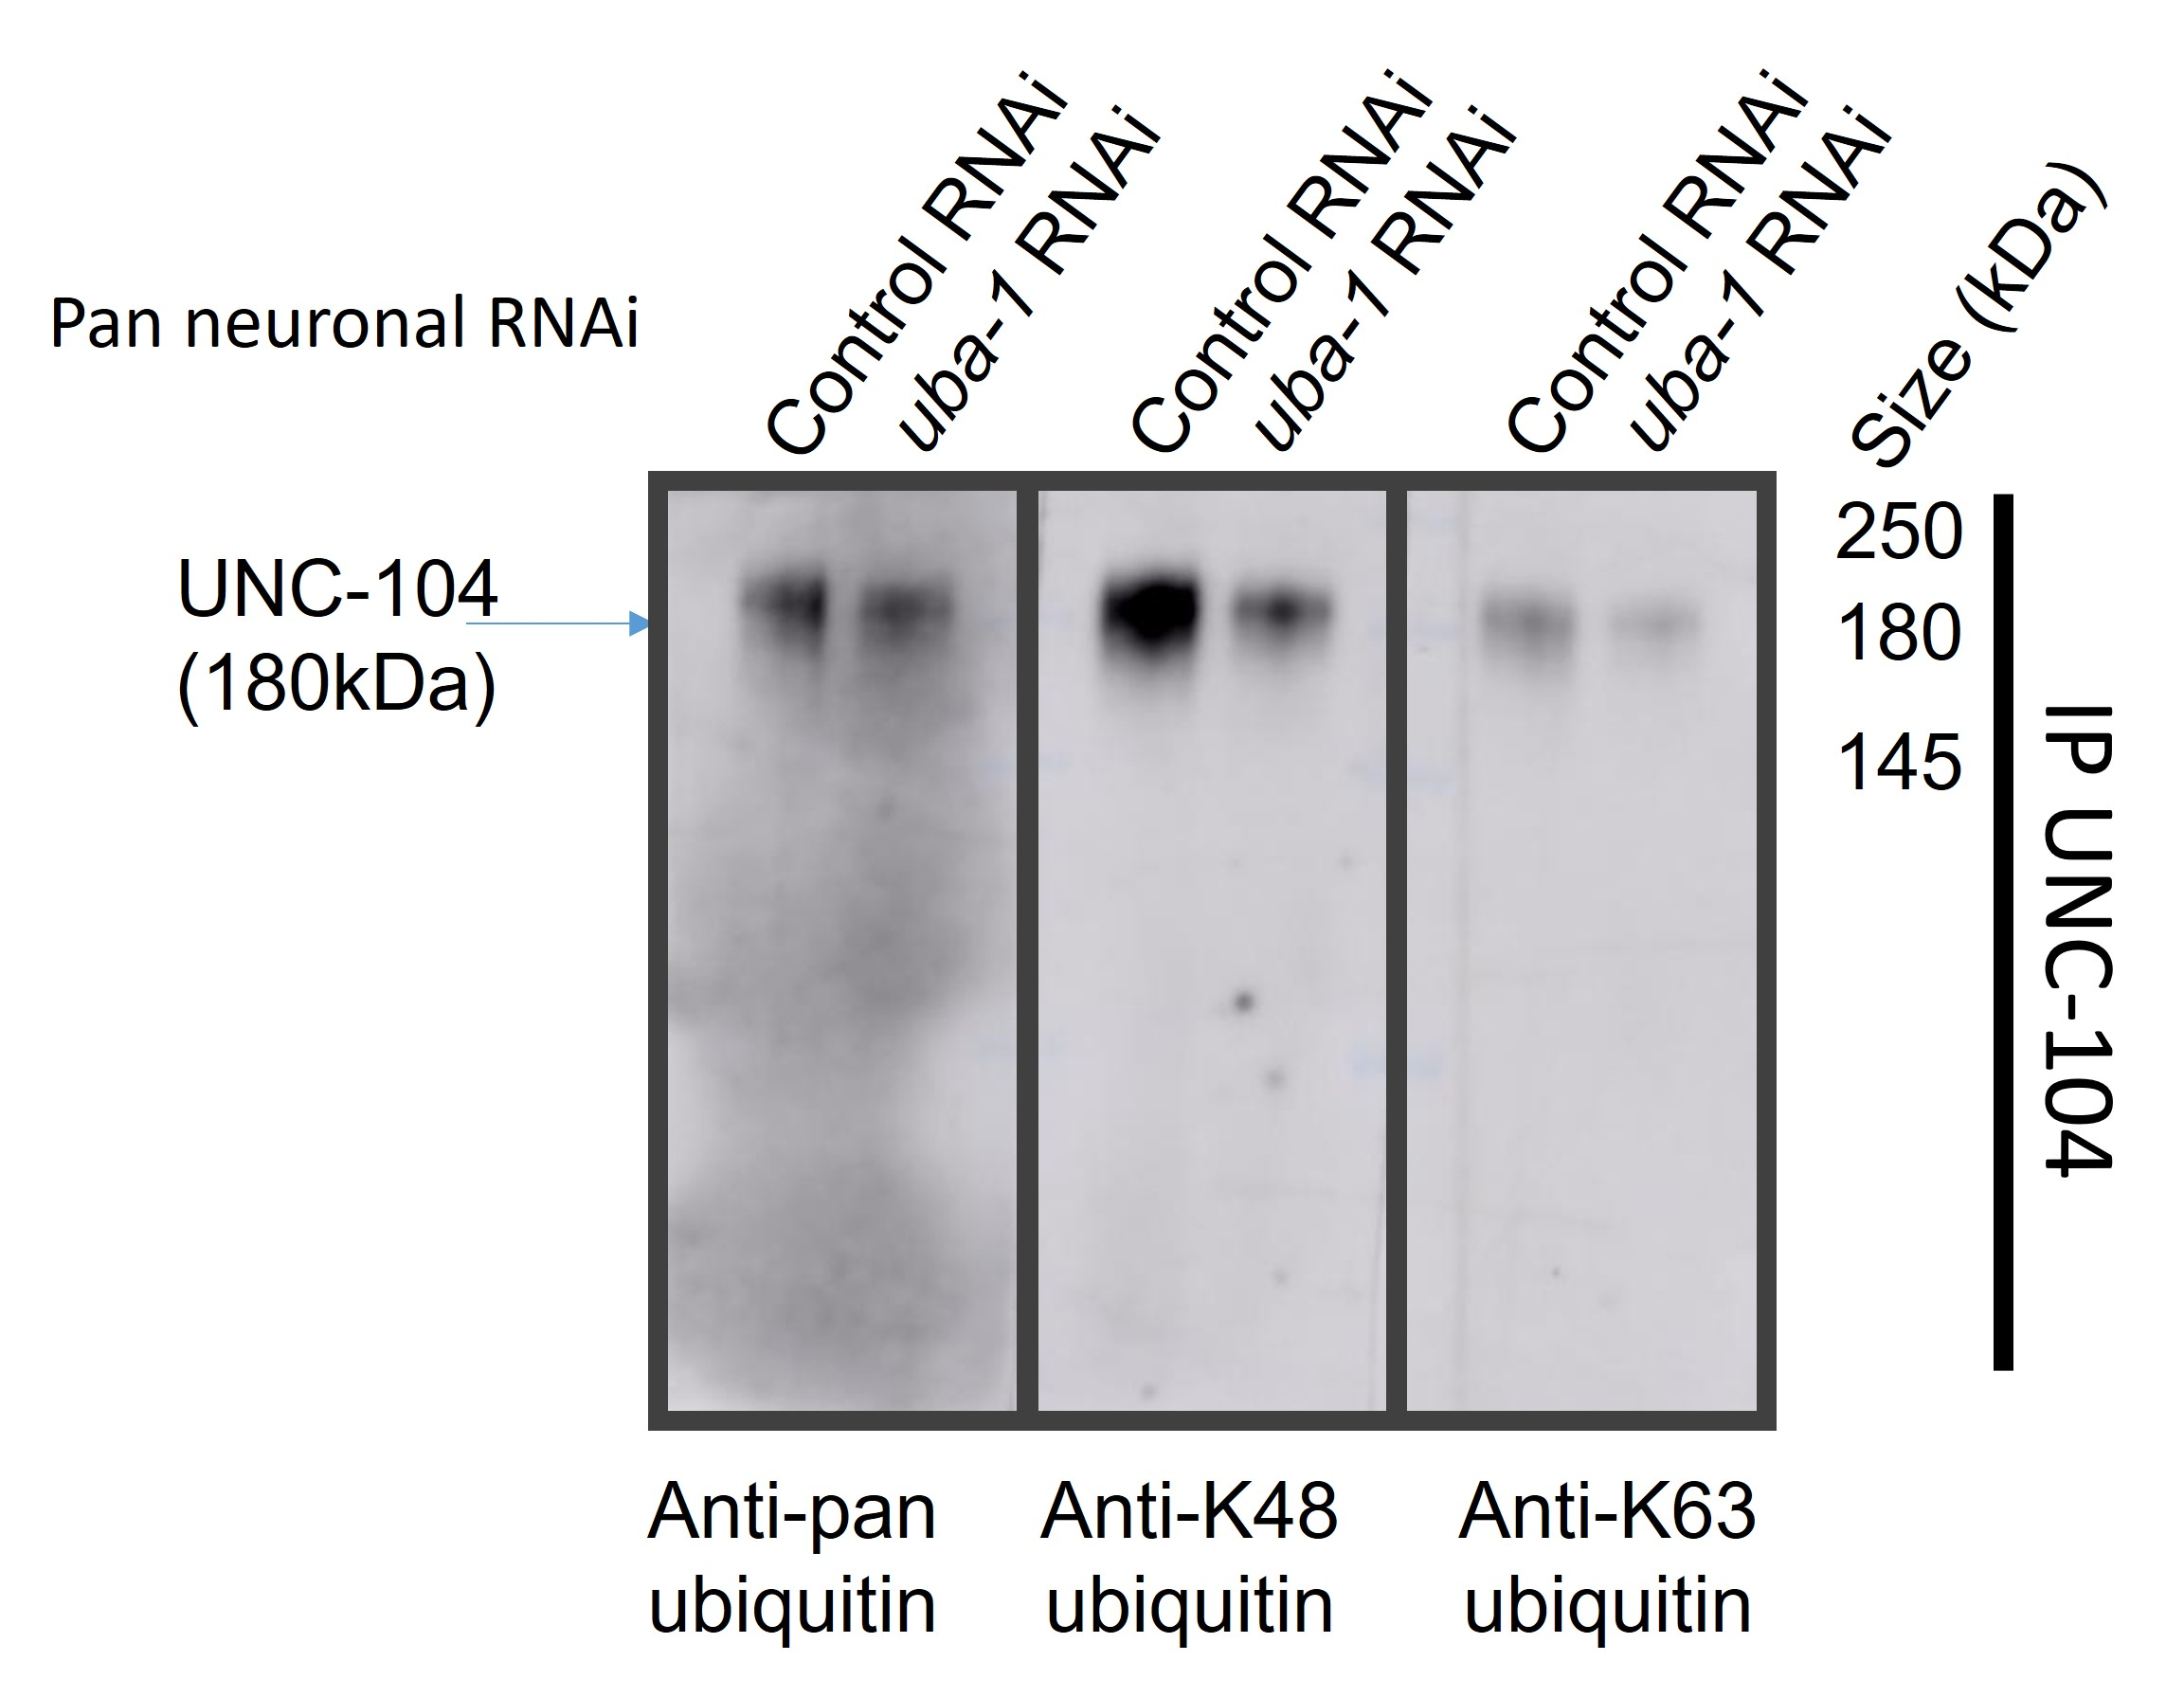
\includegraphics[width=\textwidth]{figs/example}
			
		\end{subfigure}
		\begin{subfigure}{0.32\textwidth}
			\caption{}
			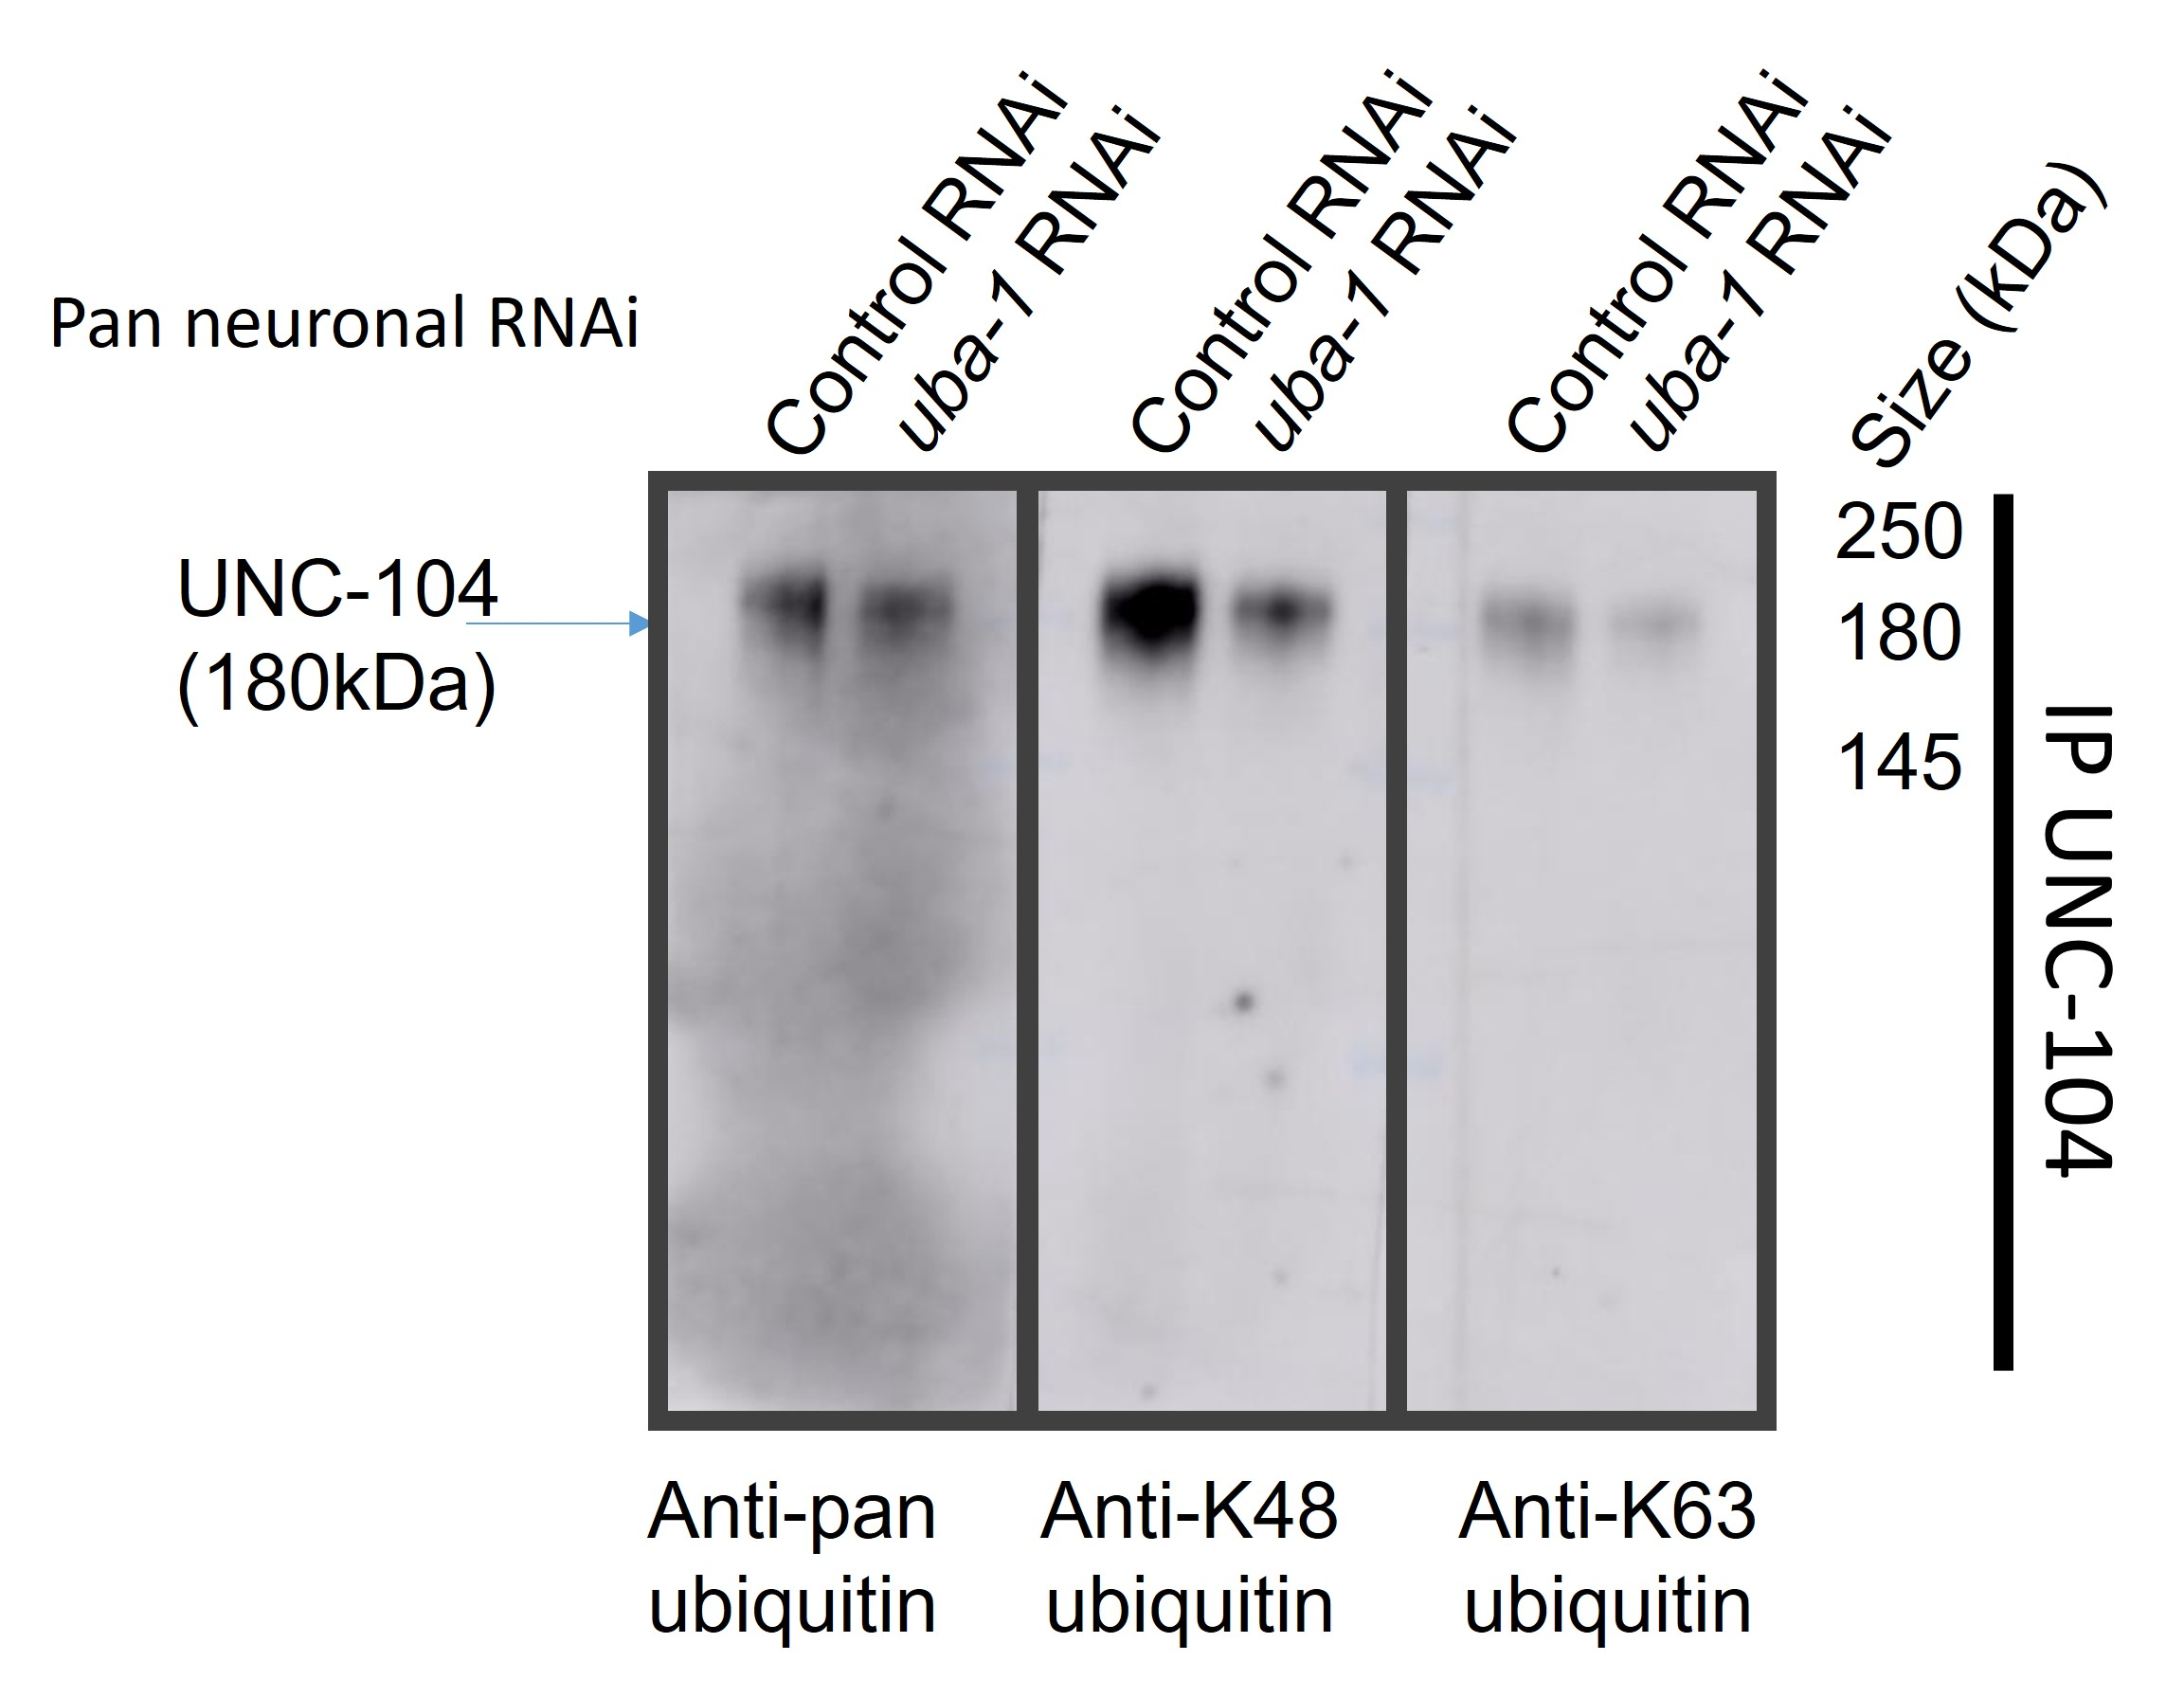
\includegraphics[width=\textwidth]{figs/example}
			
		\end{subfigure}
		
		\caption[Increase in microtubule dynamics in \textit{unc-16(lf)} are mediated through \textit{cebp-1}.]{\textbf{Increase in microtubule dynamics in \textit{unc-16(lf)} are mediated through \textit{cebp-1}.}} \raggedright \small A) Number of microtubule tracks, B) growth duration, and C) polymerization length of microtubule tracks assessed using EBP-2::GFP comets in the uncut (U), or 6 hrs post ablation (6) in wild type, \textit{cebp-1(lf)}, \textit{unc-16(lf)}, or the double \textit{unc-16(lf), cebp-1(lf)}. Bar graphs represent the average with the whiskers representing S.E.M. for the number of animals written on the bottom of the bar. One-way ANOVA was used for statistical analysis with all comparisons made with the 0 hr data for each genotype. *p$<$0.05, **p$<$0.01, ***p$<$0.001.
		\label{fig:MTdyncebp}
	\end{figure}
	
	\subsection{Actin dynamics alter 3 hours post injury}
	
	While the dynamics of microtubules post injury was already characterized, actin dynamics were largely studied at the growth cone or inferred from waves moving throughout the neuronal process \parencite{difato2011, leite2021}. Thus, to understand how actin is regulated throughout the neuronal process, we utilized a GFP tagged \textit{Drosophila} utrophin calponin homology (GFP::utCH) to assess actin dynamics within the neuronal process. We first did a time course of 1, 2 and 3 hours post ablation to observe the change in actin dynamics at a similar timescale as that of microtubules. We observed that the anterograde and retrograde polymerizing actin was largely similar across different time points, with an increase in the number of GFP::utCH trails increasing significantly 3 hours post ablation [Fig.~\ref{fig:Actdyntime}A]. In contrast, similar to what was observed in the case of microtubule dynamics, the total length to which GFP::utCH trails grew was significantly higher 2 hours post ablation [Fig.~\ref{fig:Actdyntime}A]. There was also a corresponding decrease in the number of stationary GFP::utCH events 1 hour post ablation, and a decrease in the duration of the stationary events 3 hours post ablation [Fig.~\ref{fig:Actdyntime}C,D]. These data together suggest that, similar to microtubule dynamics, actin dynamics are altered sequentially, with the number of stationary GFP::utCH clusters reducing first, followed by an increase in polymerizing length of the actin trails in 2 hours, followed by an increase in the number of polymerizing events 3 hours post injury.
	
		\begin{figure}[H]
		\centering
		\begin{subfigure}{0.45\textwidth}
			\caption{}
			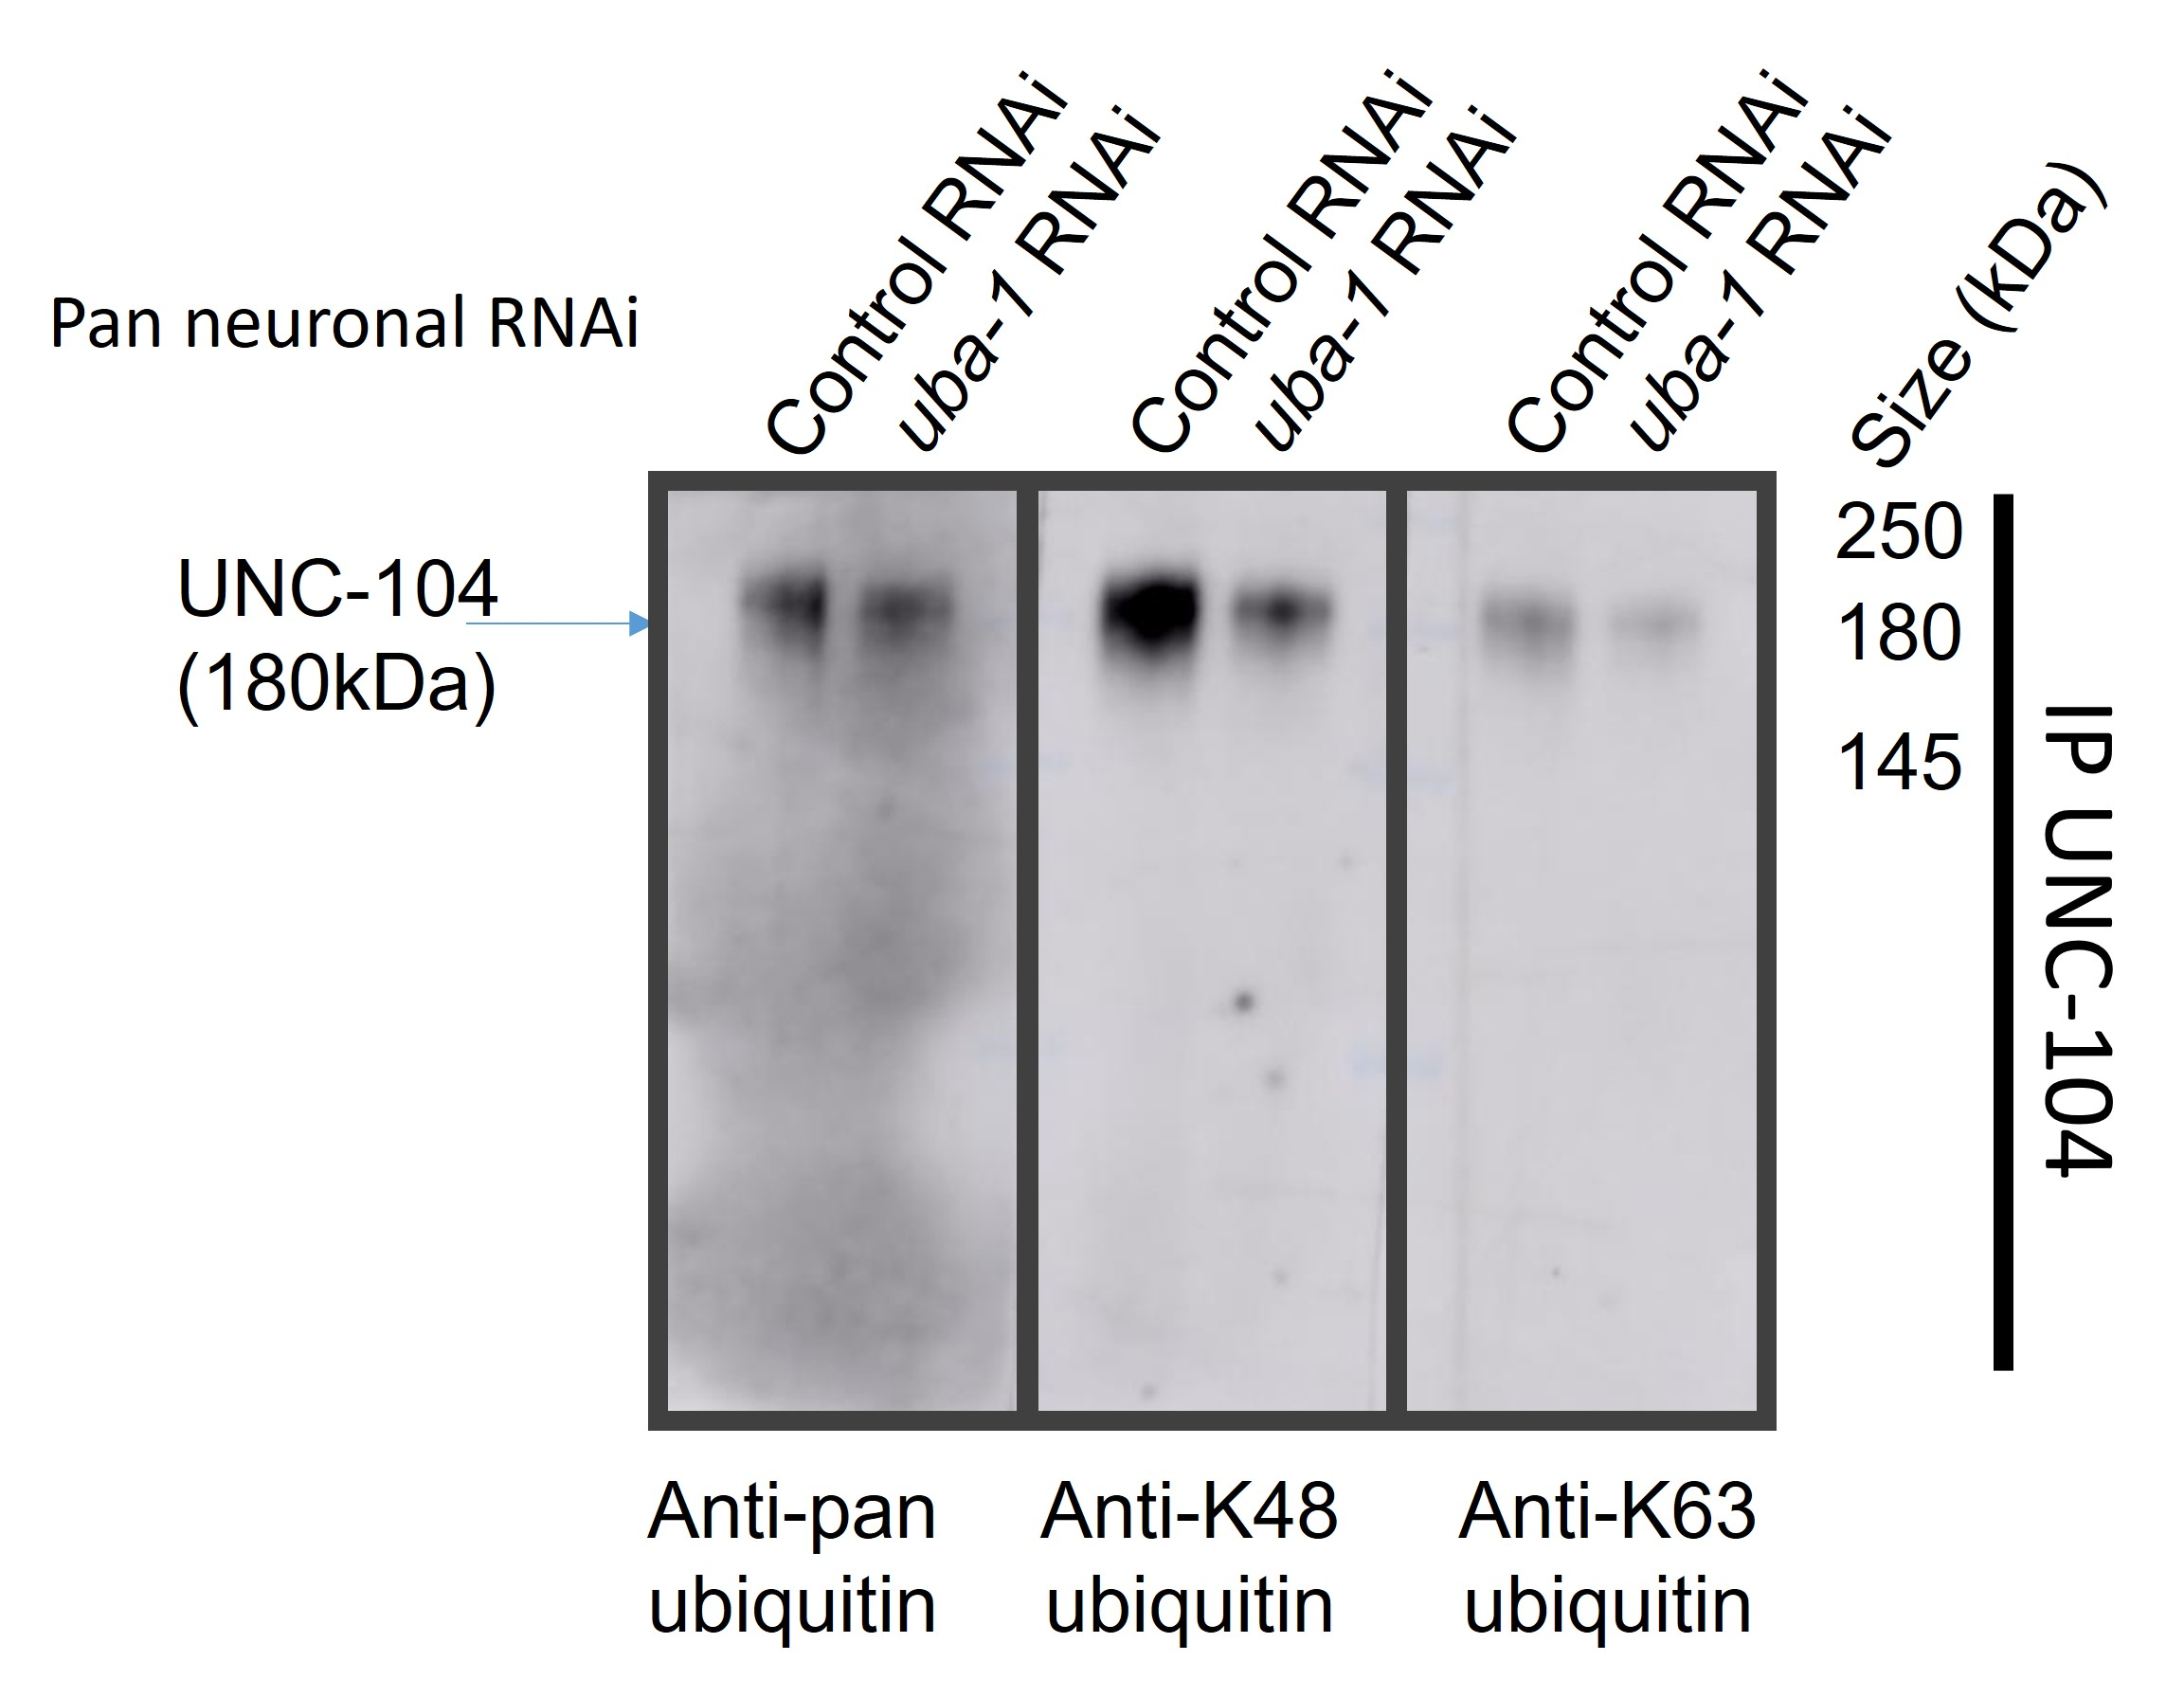
\includegraphics[width=\textwidth]{figs/example}
			
		\end{subfigure}
		%	\hfill
		\begin{subfigure}{0.45\textwidth}
			\caption{}
			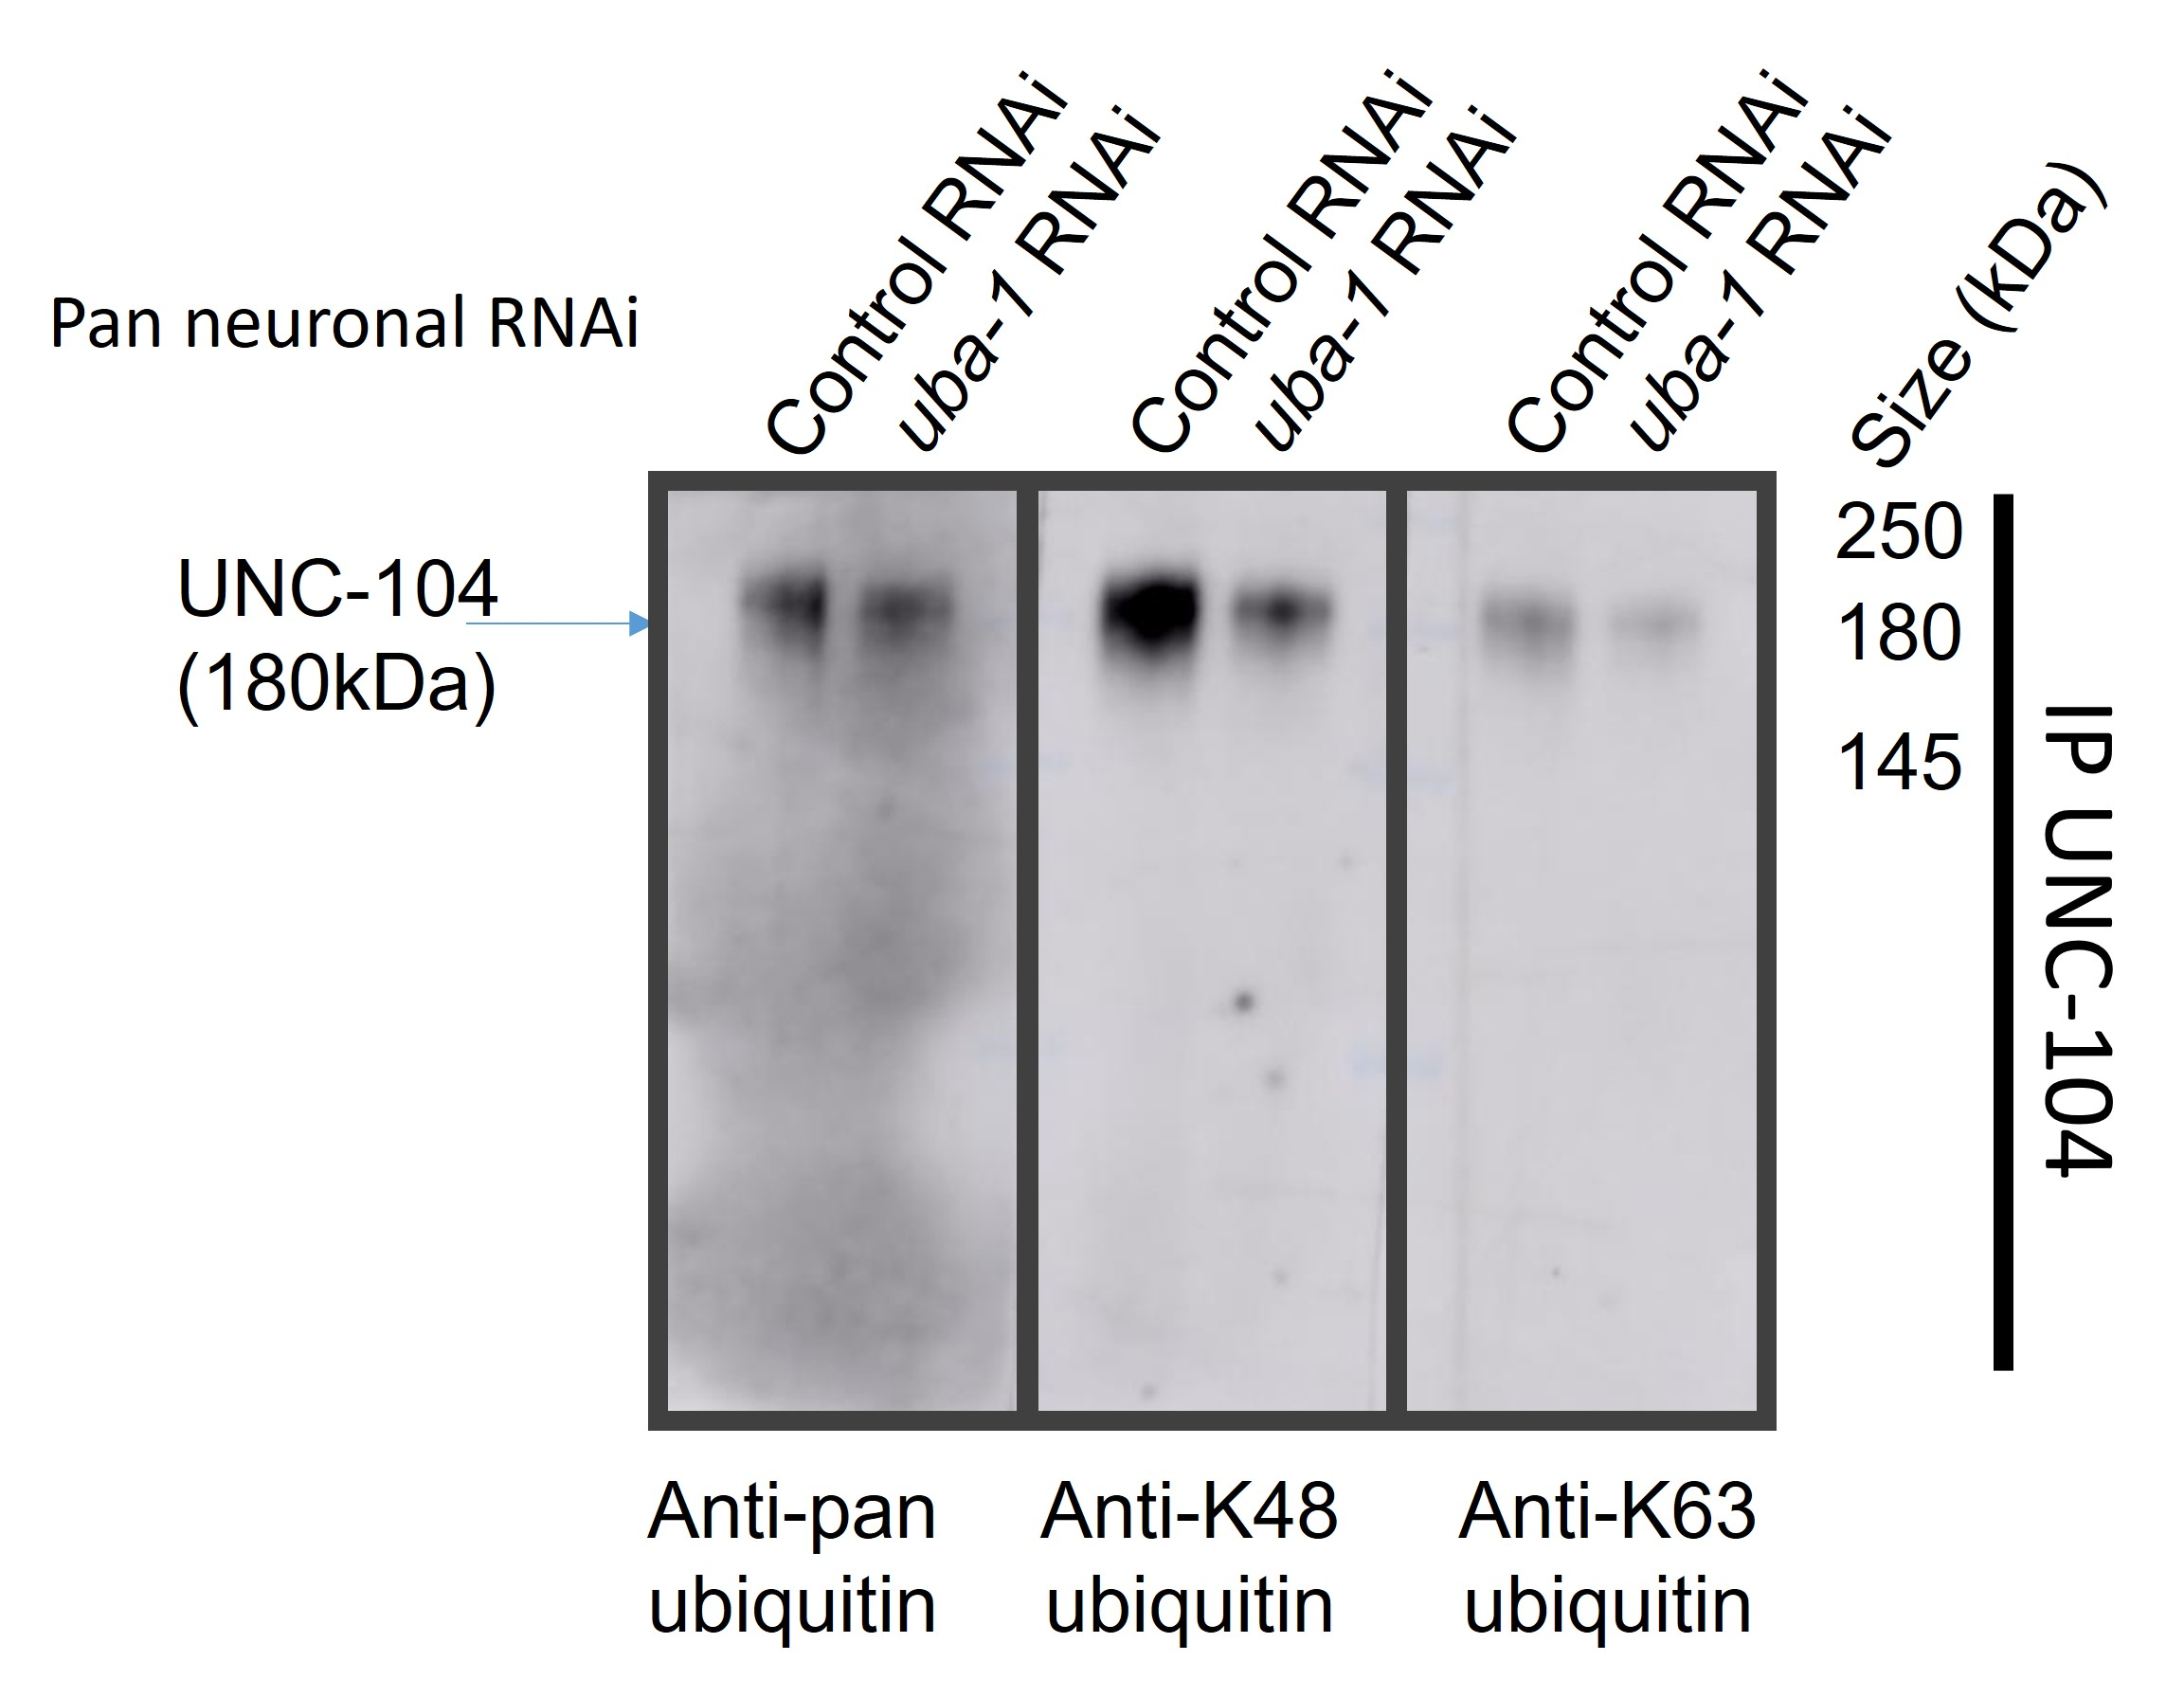
\includegraphics[width=\textwidth]{figs/example}
			
		\end{subfigure}
		\begin{subfigure}{0.45\textwidth}
			\caption{}
			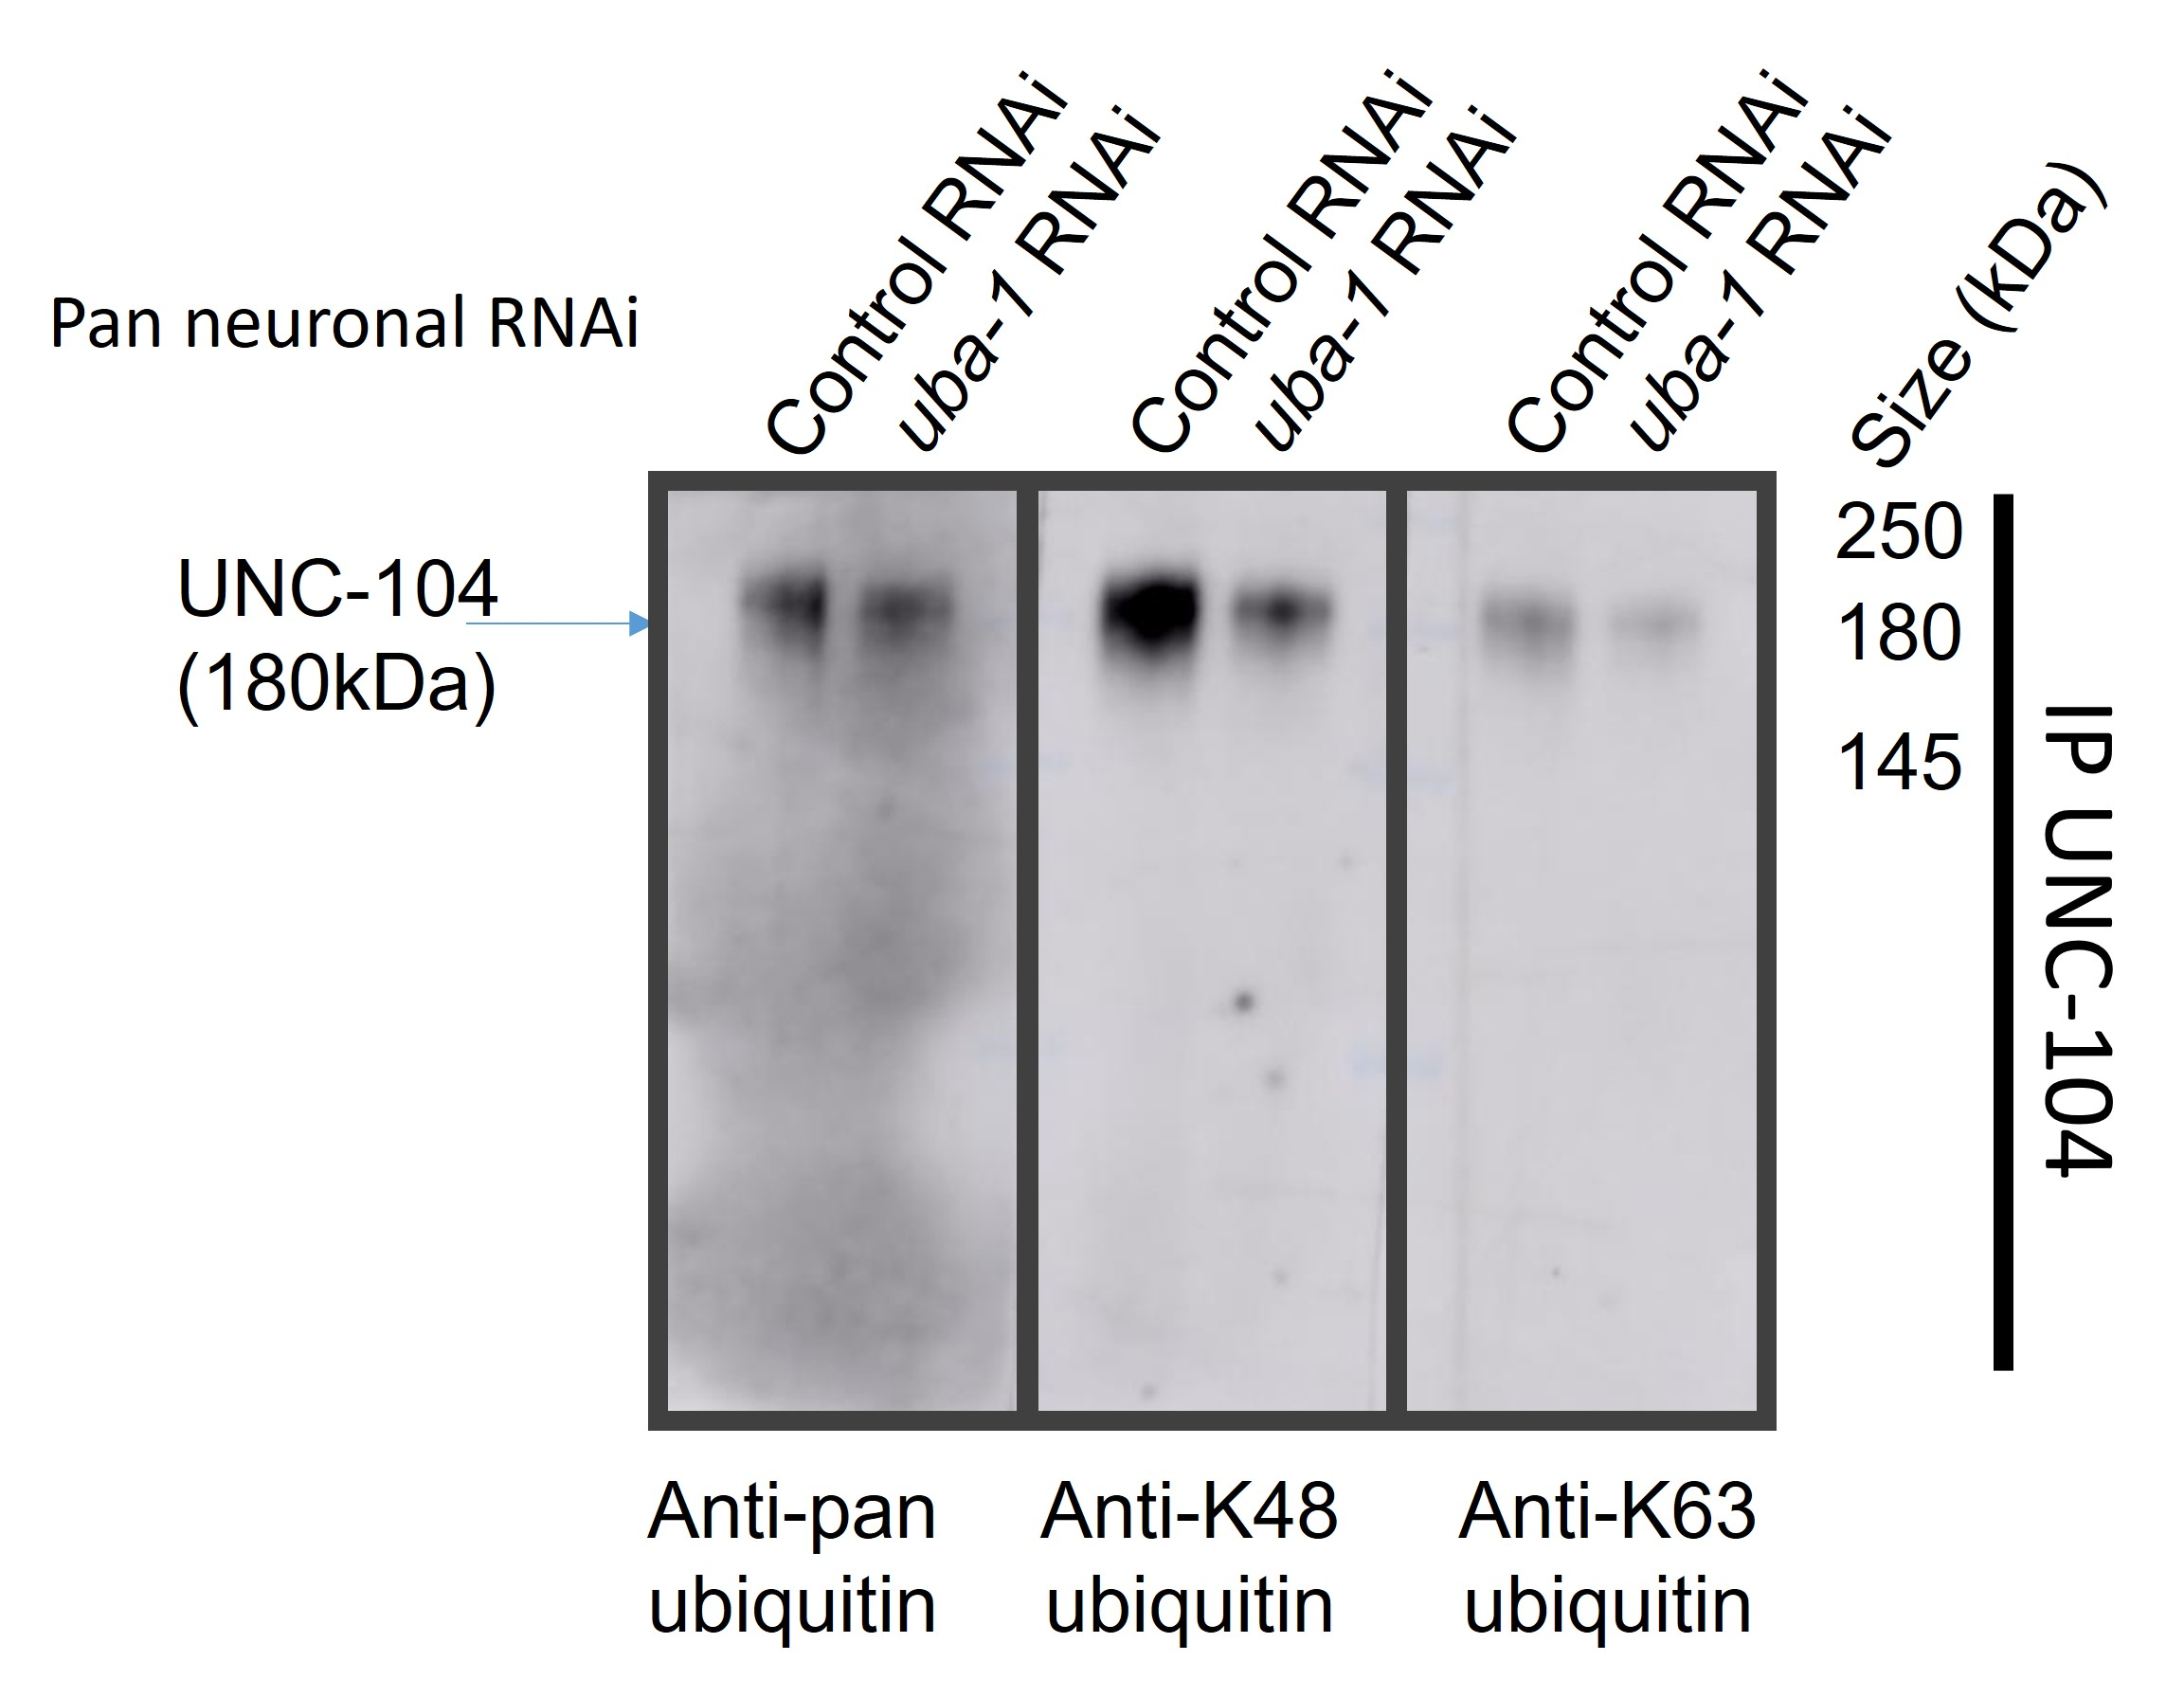
\includegraphics[width=\textwidth]{figs/example}
			
		\end{subfigure}
		\begin{subfigure}{0.45\textwidth}
			\caption{}
			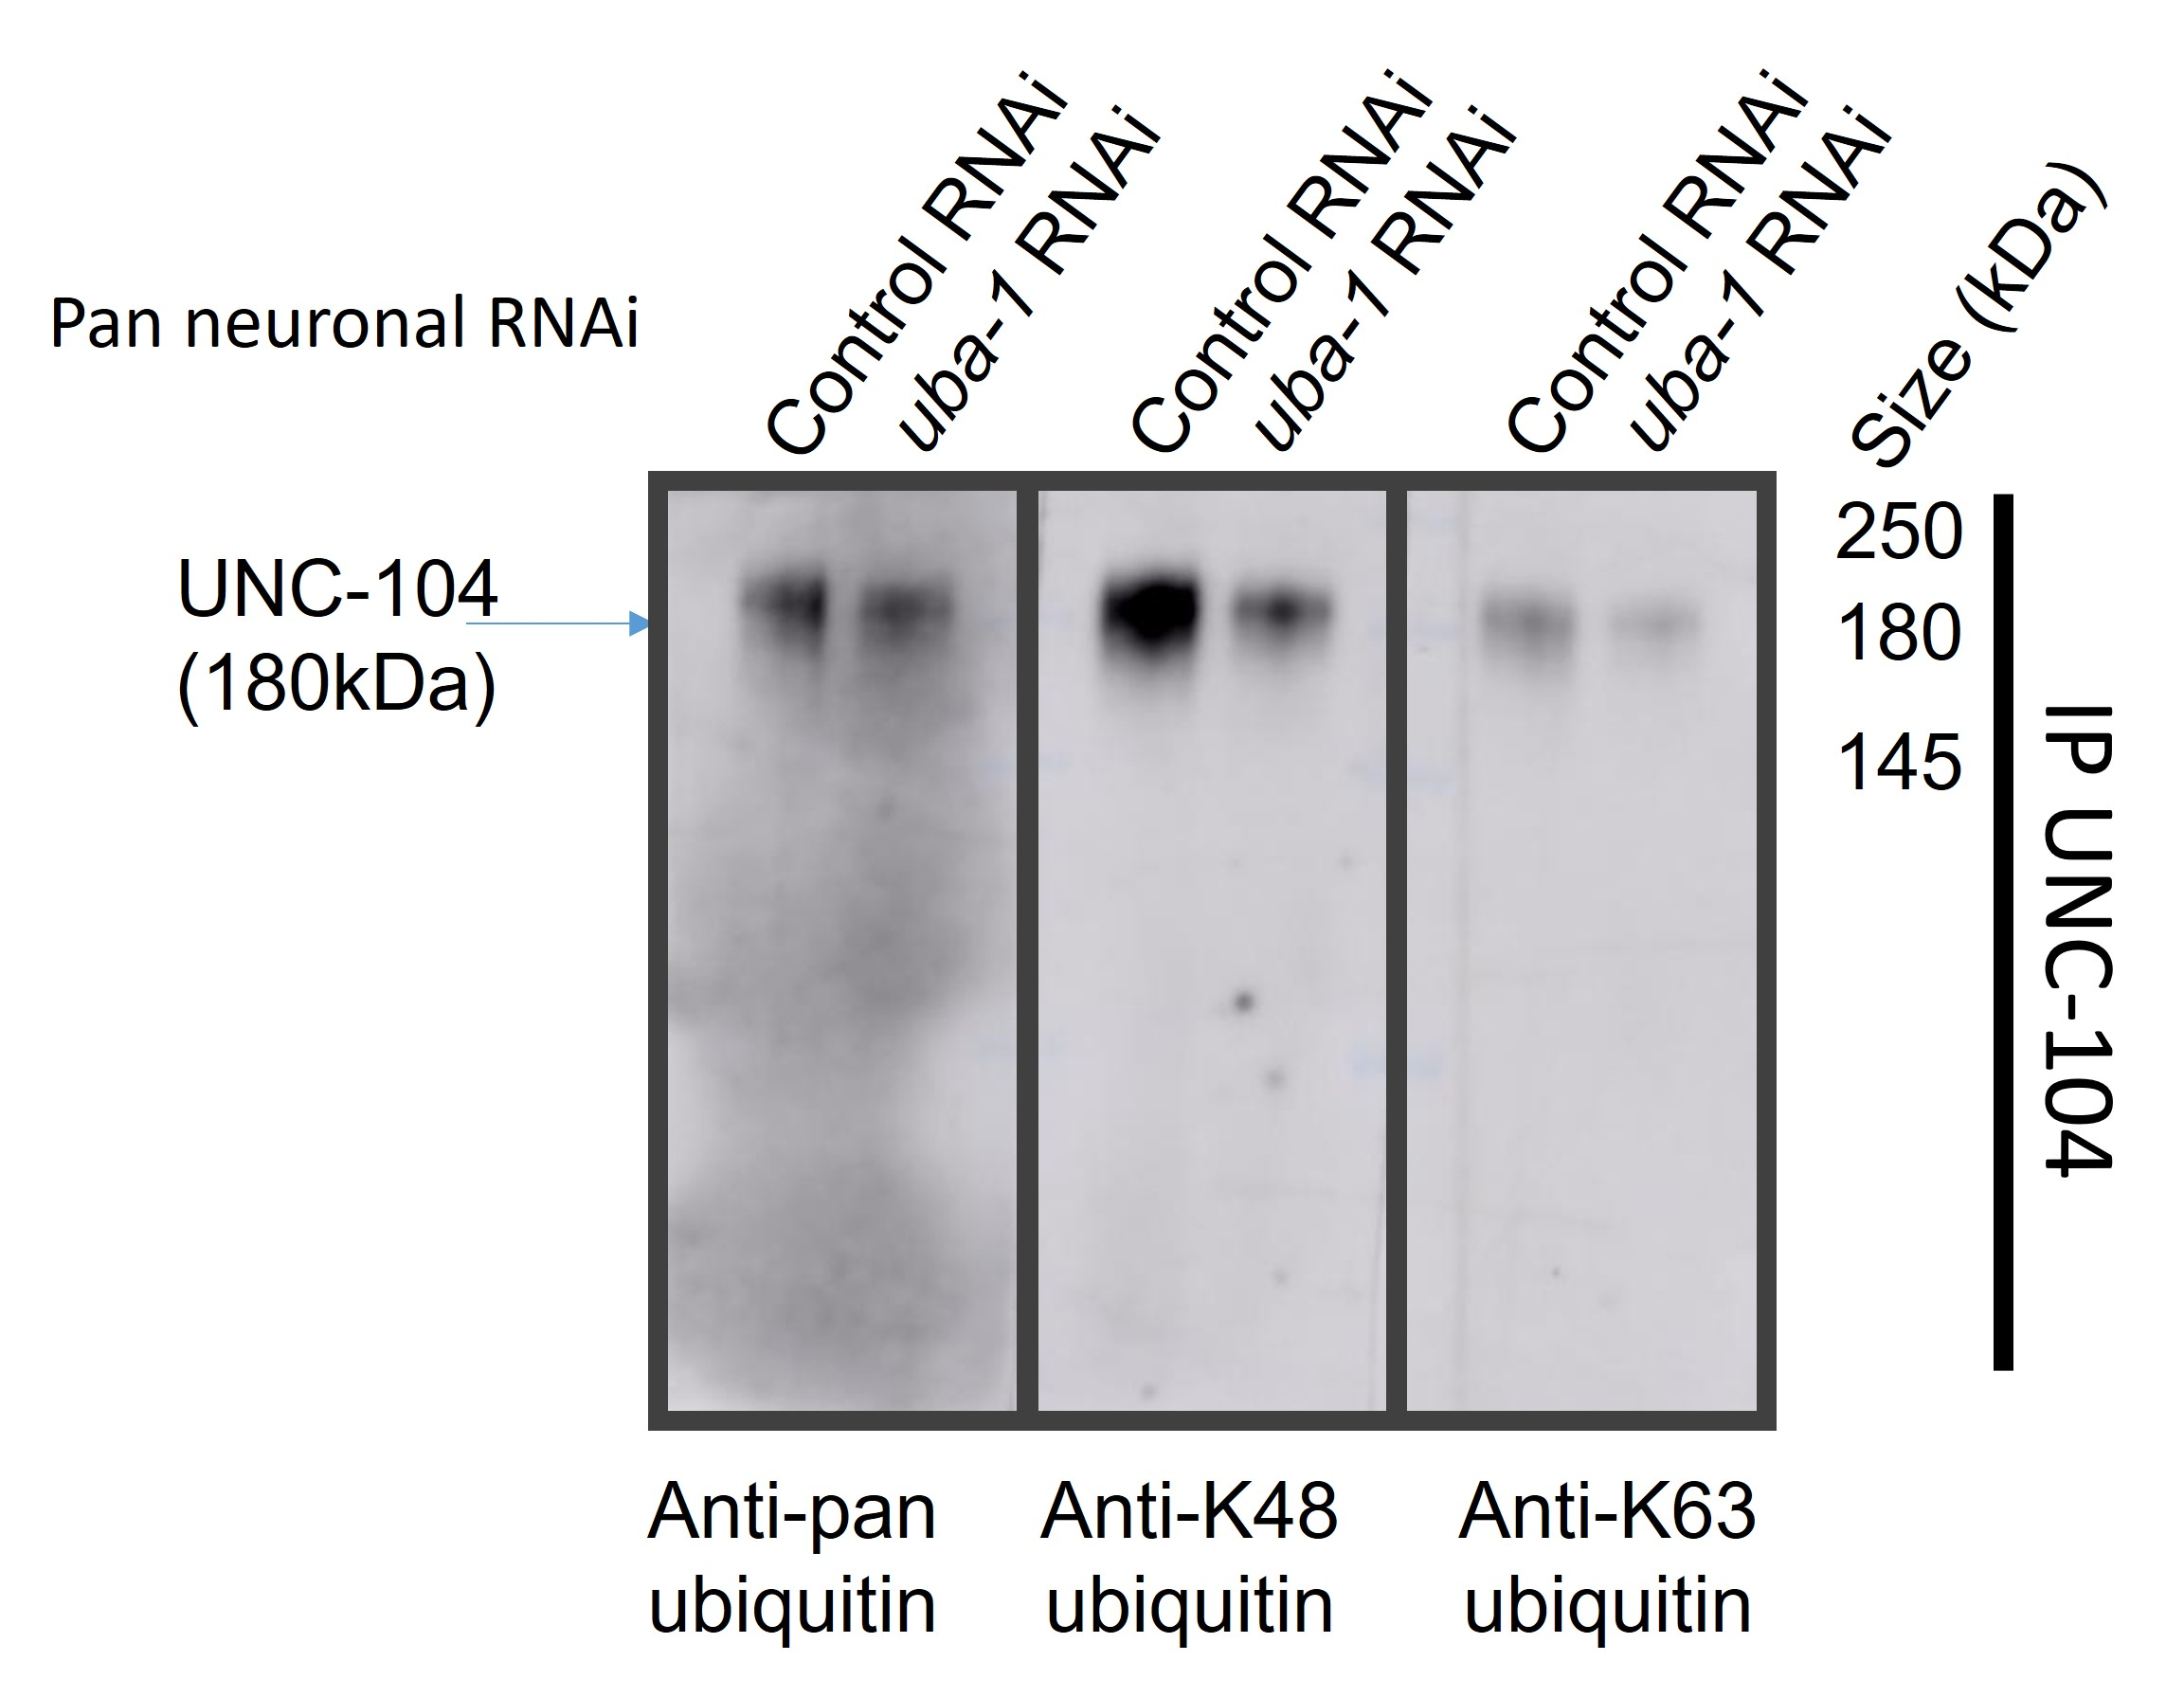
\includegraphics[width=\textwidth]{figs/example}
			
		\end{subfigure}
		
		\caption[Actin dynamics increase 3 hrs post injury.]{\textbf{Actin dynamics increase 3 hrs post injury.}} \raggedright \small A) Number and B) polymerization length of actin trails assessed using GFP::utCH in uncut (U), 1 hr, 2 hrs, and 3 hrs post ablation in wild type in the anterograde (black) and retrograde (gray) directions. C) The duration and D) density of GFP::utCH stationary clusters assessed in kymographs made from 3 min long movies in uncut (U), 1 hr, 2 hrs, and 3 hrs post ablation in wild type animals. Bar graphs represent the average of at least 15 animals with the whiskers representing S.E.M. One-way ANOVA was used for statistical analysis with all comparisons made with the uncut data for each genotype. **p$<$0.01, ***p$<$0.001.
		\label{fig:Actdyntime}
	\end{figure}
	
	\subsection{Increased actin dynamics in \textit{unc-16(lf)} post injury depends on \textit{dlk-1} and \textit{cebp-1}}
	
	As mentioned previously, DLK-1 promotes regeneration by two arms, by signaling to the nucleus via CEBP-1, and via locally regulating protein activity such as KLP-7 and CCPP-6. We thus tested how actin dynamics are regulated by \textit{unc-16} and \textit{dlk-1}. We observed that the baseline number of GFP::utCH trails were largely similar in all mutants tested [Fig.~\ref{fig:Actdynmut}A], however the baseline length of the polymerizing GFP::utCH trails were significantly higher for the \textit{unc-16(lf)} mutant [Fig.~\ref{fig:Actdynmut}B]. The velocity of GFP::utCH trails was largely similar across different mutants as well [Fig.~\ref{fig:Actdynmut}C]. The number of baseline stationary GFP::utCH events was significantly reduced in \textit{unc-16(lf)} [Fig.~\ref{fig:Actdynmut}D]. 3 hours post injury, while neurons in wild type animals displayed an increase in number, polymerizing length and decrease in stationary GFP::utCH events, \textit{dlk-1(null)} mutants did not have any change in these properties compared to the uninjured neurons. In contrast, \textit{unc-16(lf)} mutants had a larger increase in the number of polymerizing events, while the length of the polymerizing events increased slightly and the number of stationary clusters reduced slightly. The slight but insignificant change may be due to the two features near the upper and lower limit of our ability to resolve the number of events. The double \textit{dlk-1(null)}; \textit{unc-16(lf)} and the double \textit{unc-16(lf)}; \textit{cebp-1(lf)} phenocopied their respective singles \textit{dlk-1(null)} and \textit{cebp-1(lf)} in terms of the number, length and velocity of GFP::utCH trails. In terms of the stationary GFP::utCH trails, the double \textit{dlk-1(null)}; \textit{unc-16(lf)} phenocopied the single \textit{dlk-1(null)}, but the double \textit{unc-16(lf)}; \textit{cebp-1(lf)} was in between both singles \textit{unc-16(lf)} and \textit{cebp-1(lf)}. These data  together suggest that upregulated actin dynamics in \textit{unc-16(lf)} may be regulated through \textit{dlk-1}, and may be partially regulated through \textit{cebp-1}.
	
	
	
	\begin{figure}[H]
	\begin{minipage}[t]{0.6\textwidth}
		\vspace{0pt}
		\begin{subfigure}{1\textwidth}
			\caption{}
			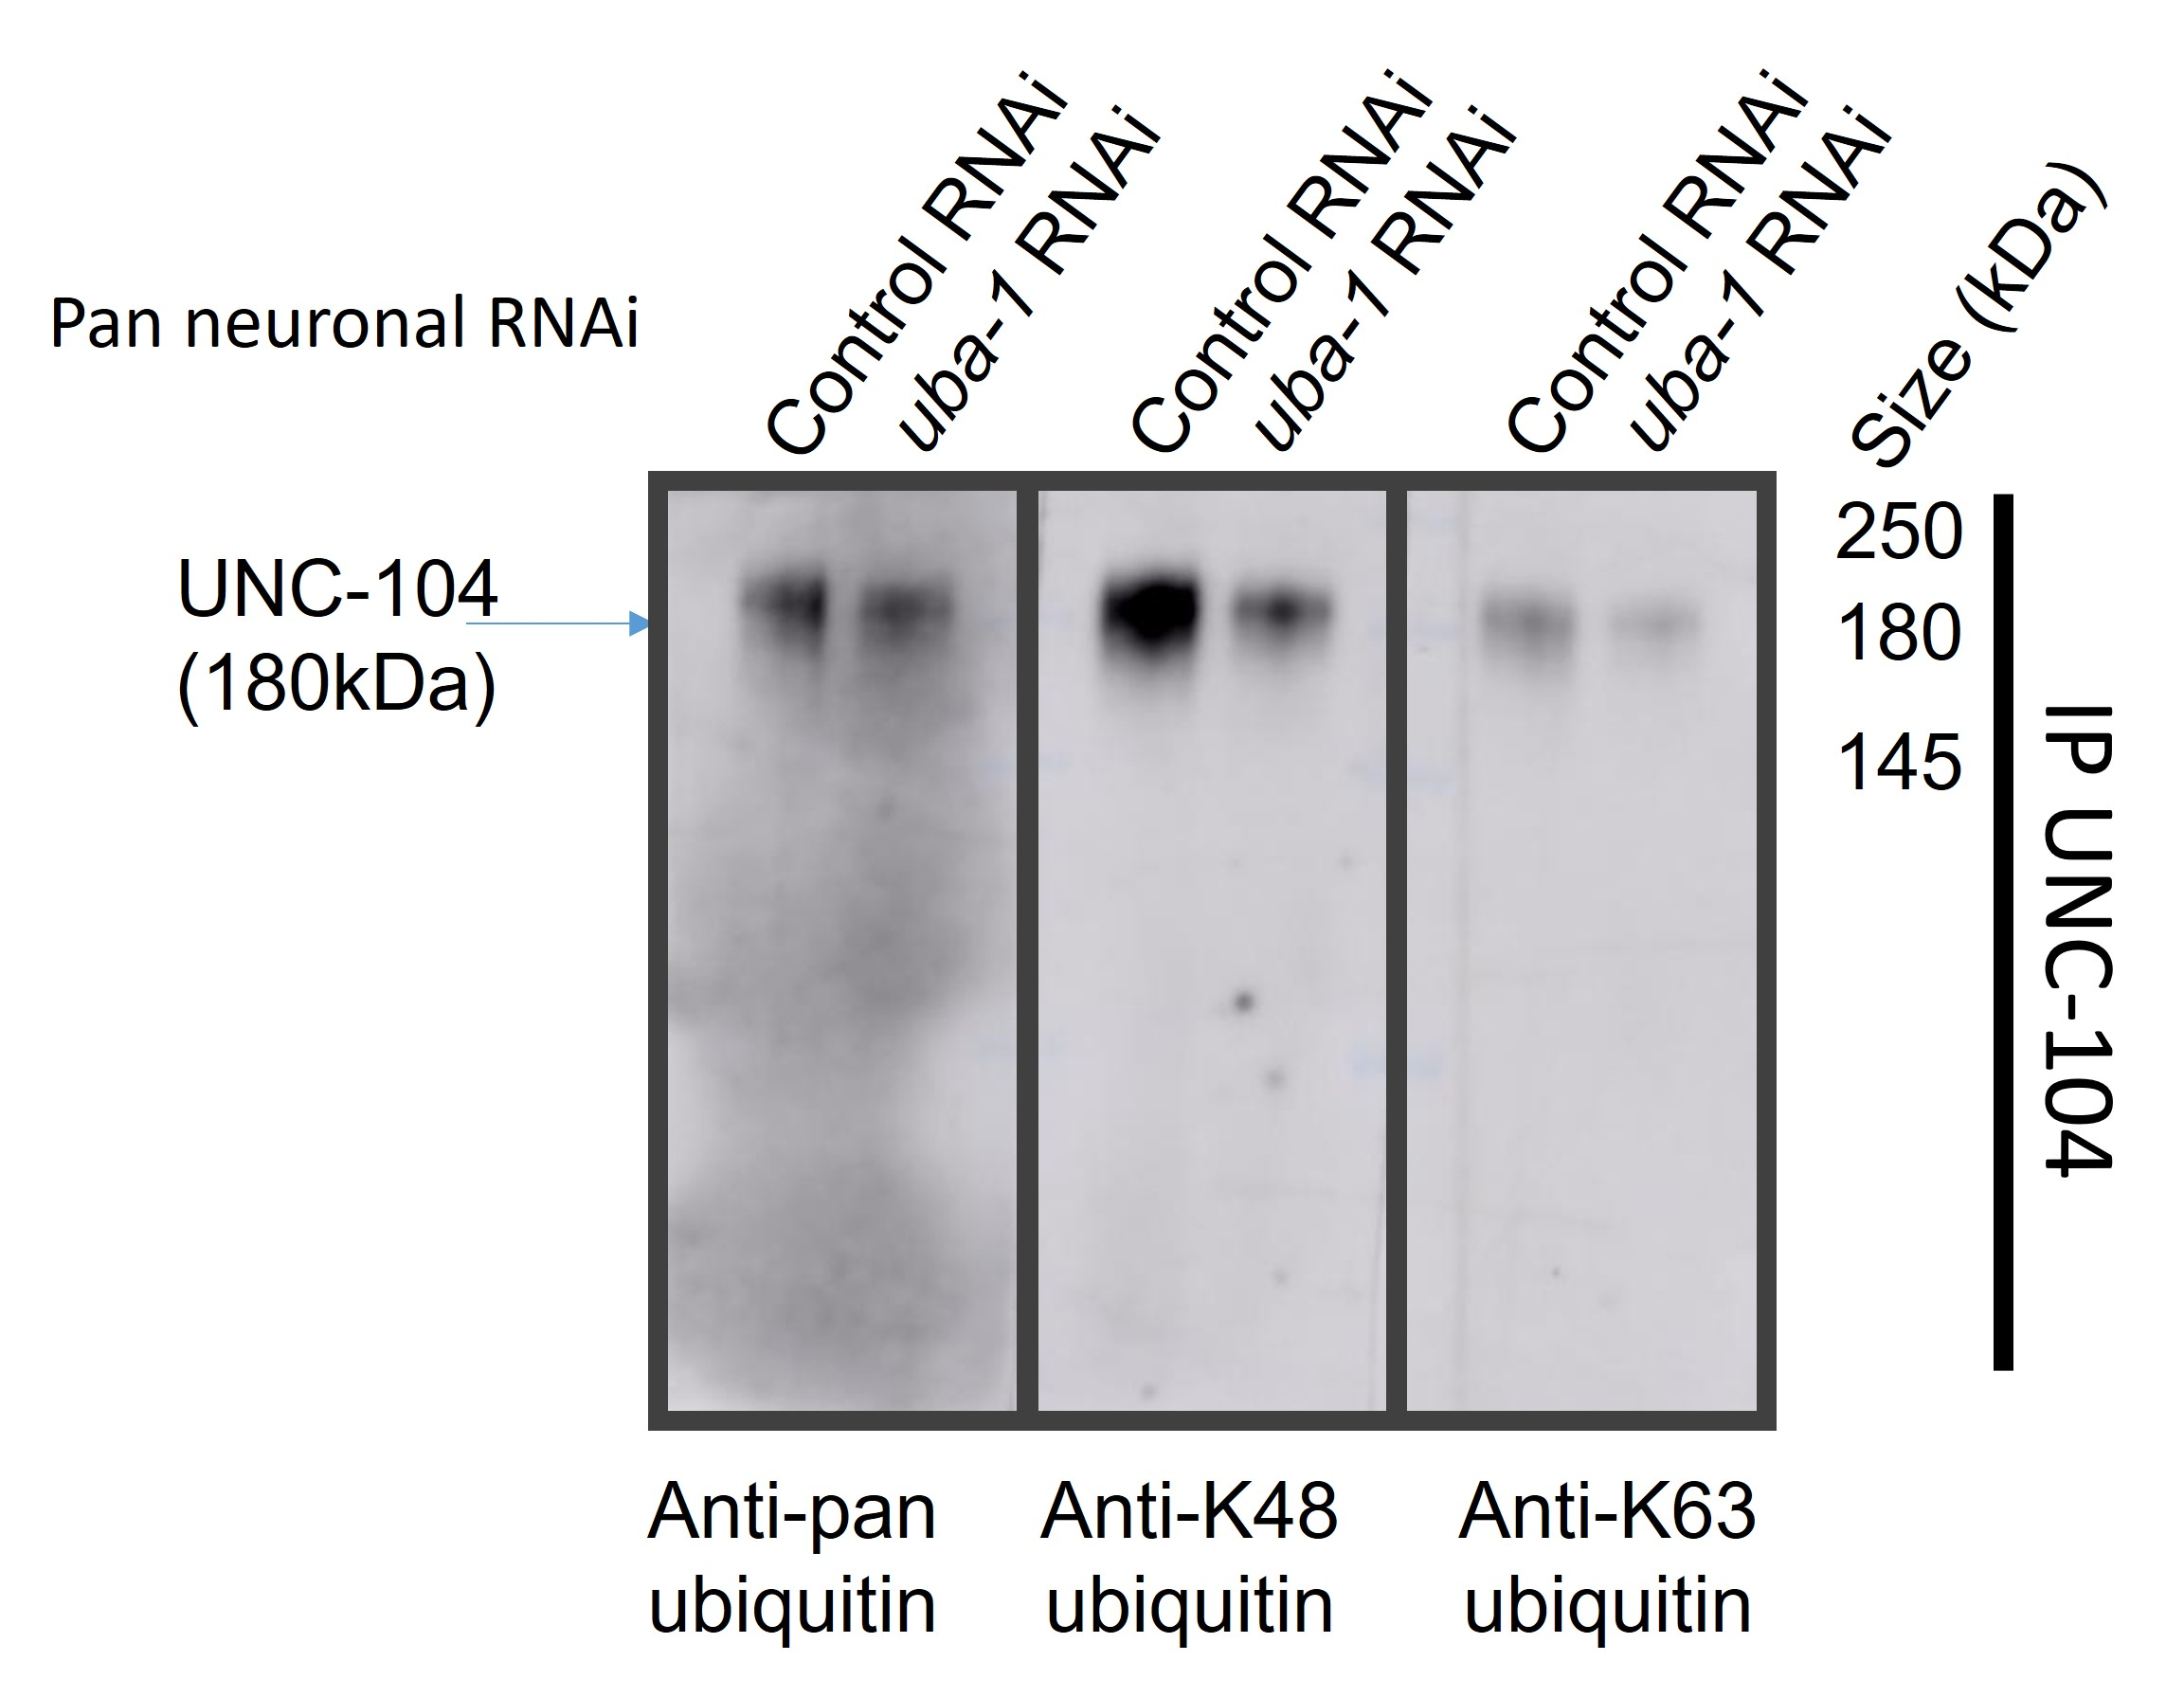
\includegraphics[width=\textwidth]{figs/example}
			
		\end{subfigure}
		%	\hfill
		\begin{subfigure}{1\textwidth}
			\caption{}
			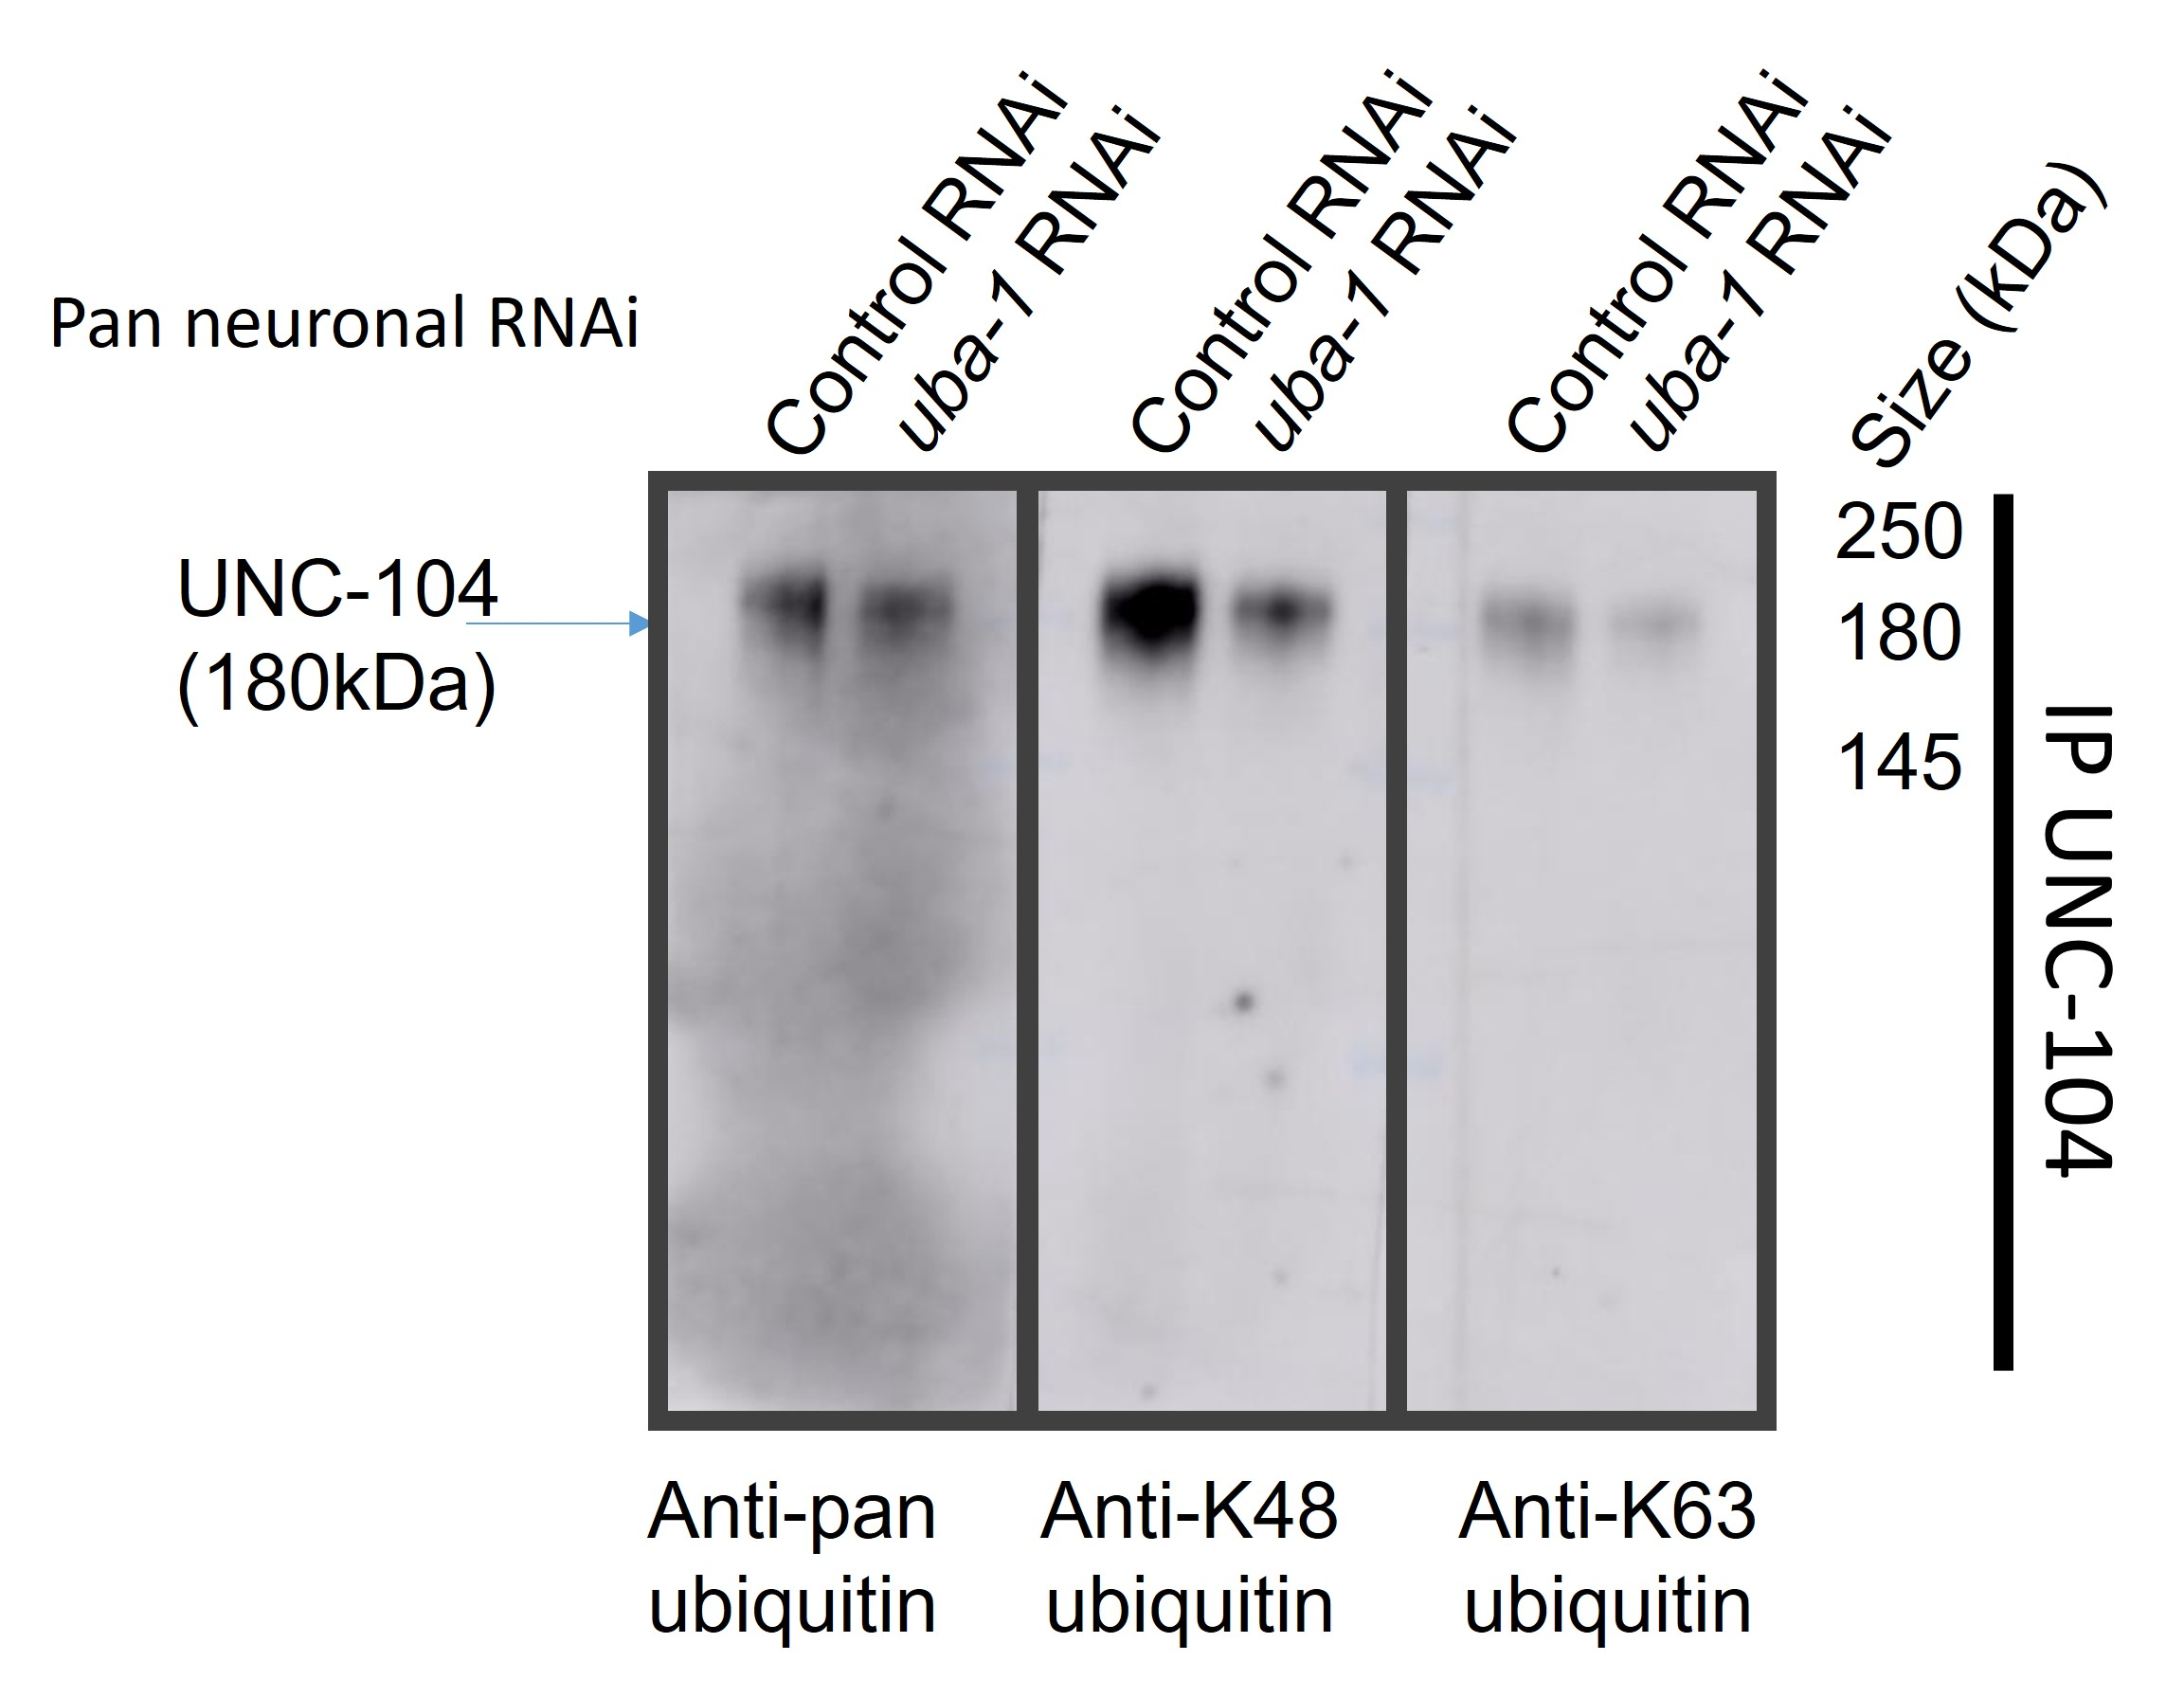
\includegraphics[width=\textwidth]{figs/example}
			
		\end{subfigure}
		\begin{subfigure}{1\textwidth}
			\caption{}
			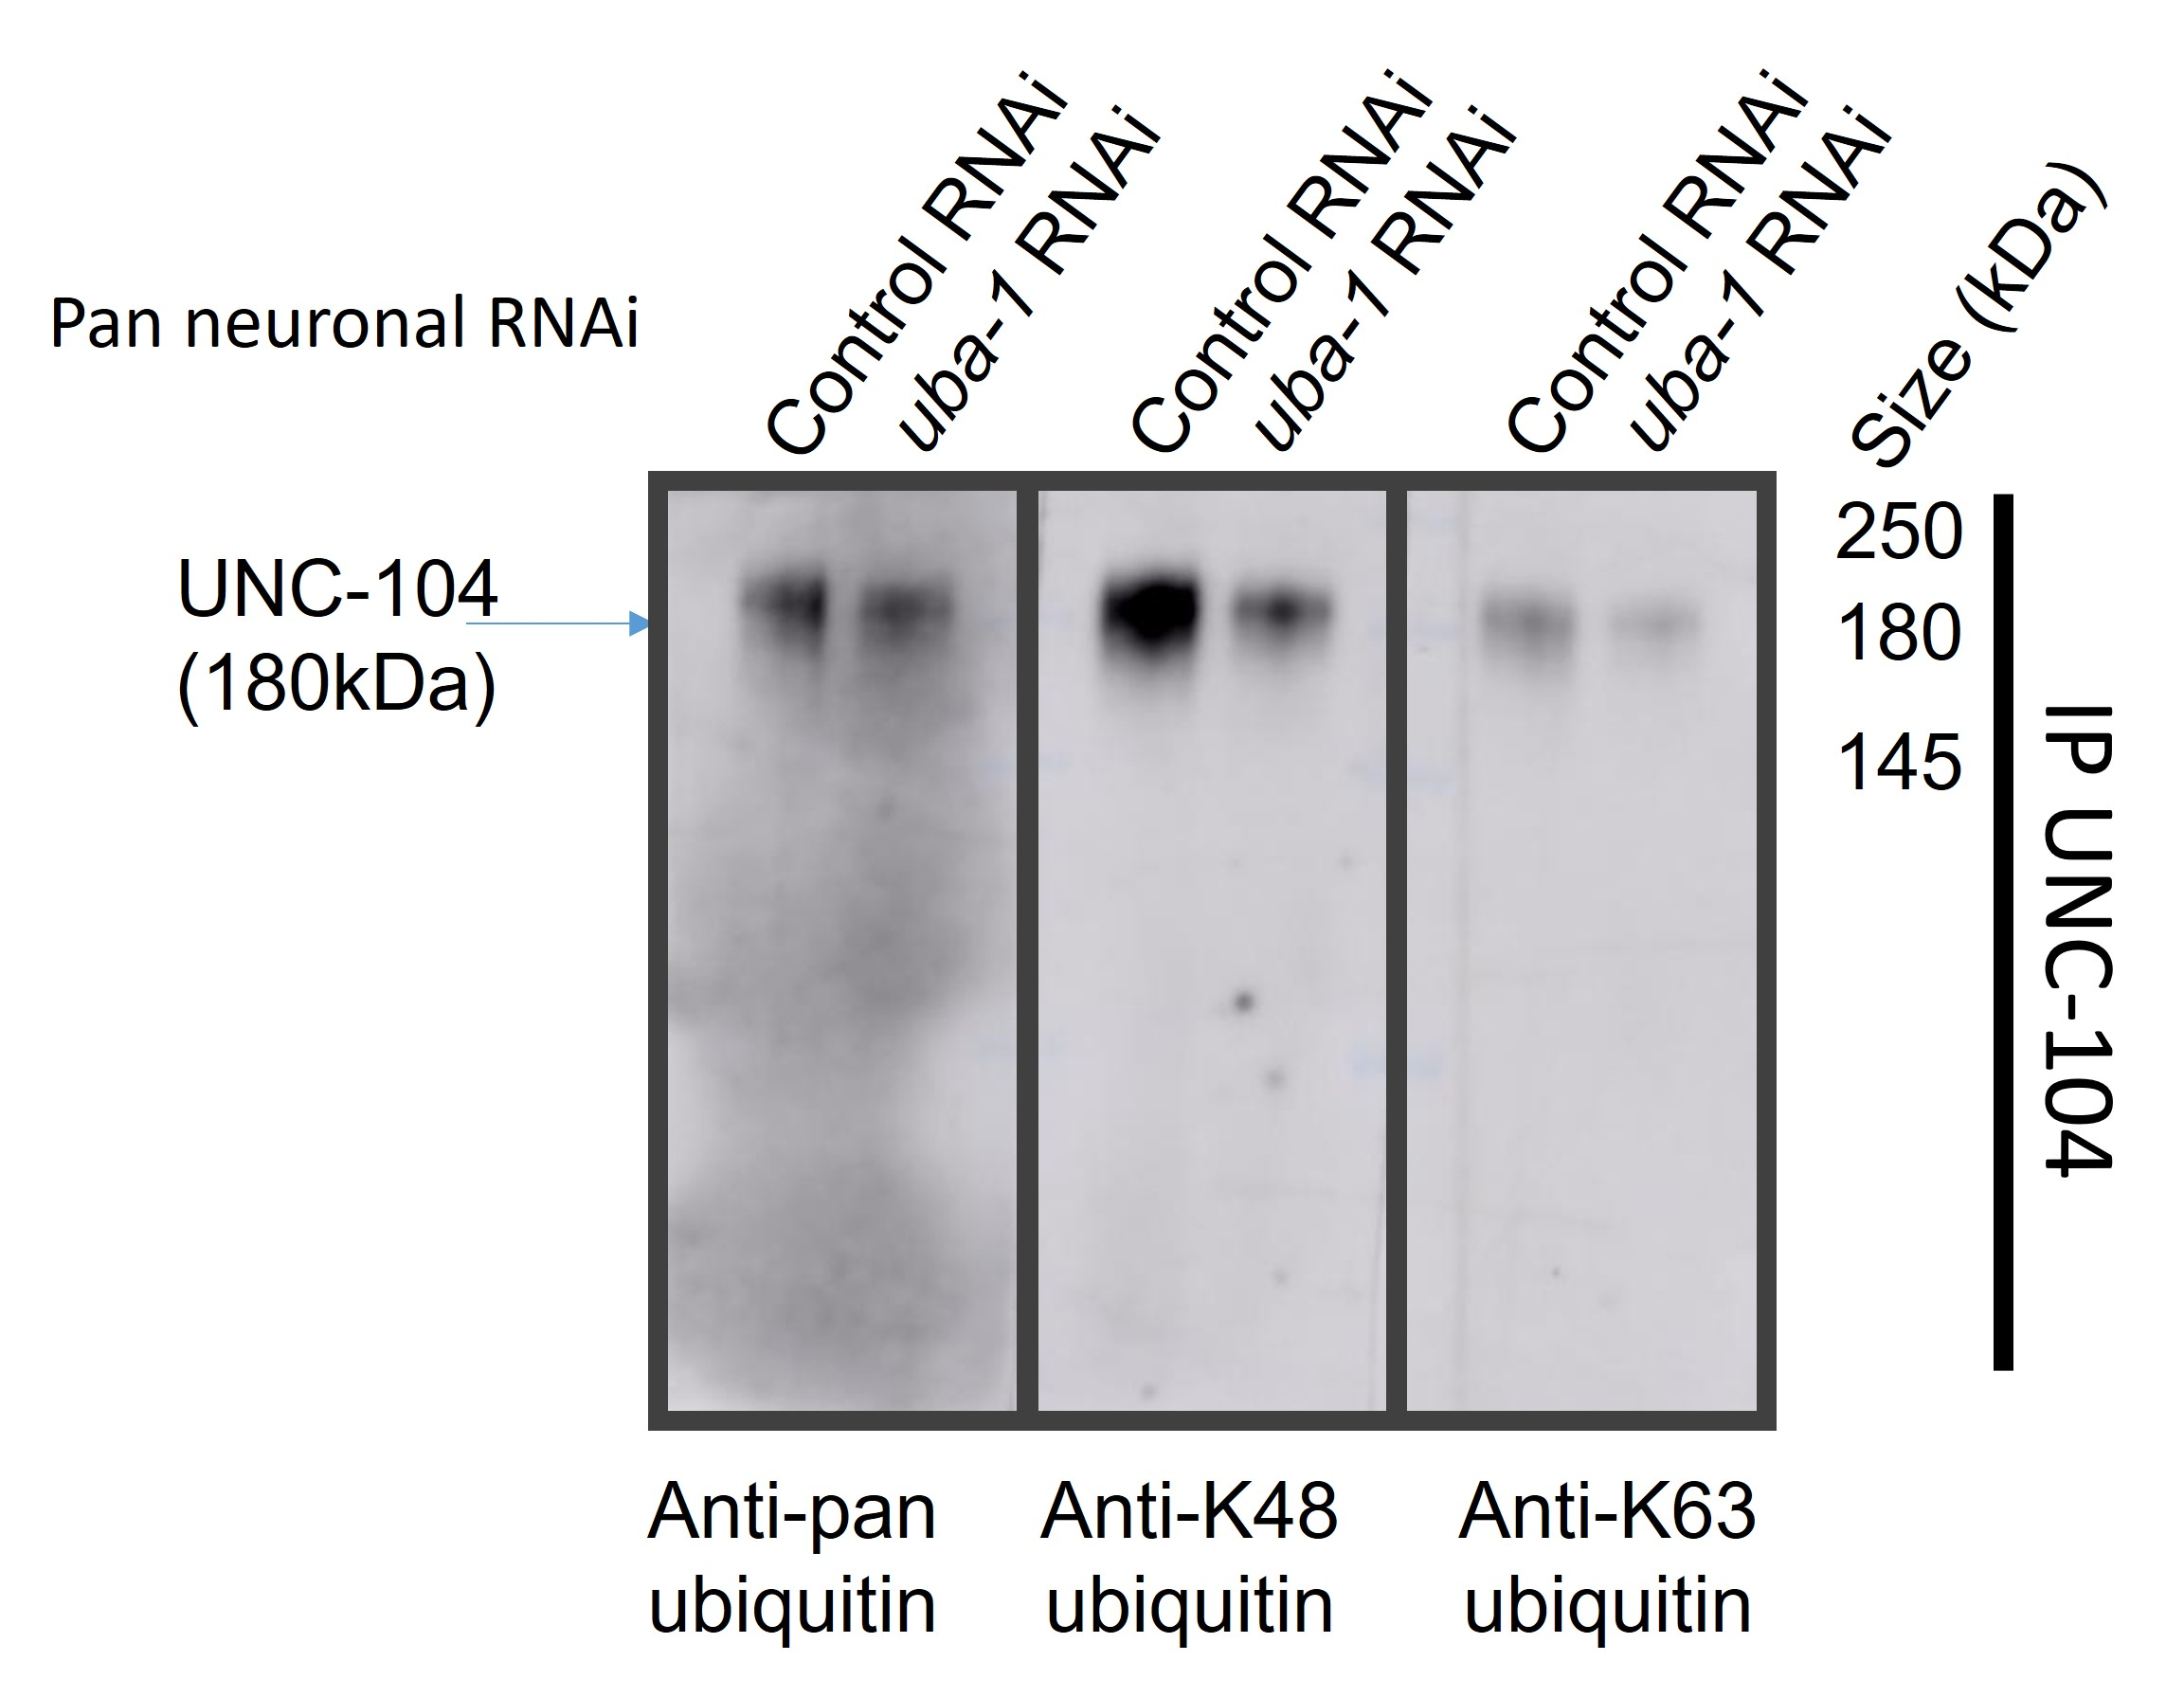
\includegraphics[width=\textwidth]{figs/example}
			
		\end{subfigure}
		\begin{subfigure}{1\textwidth}
			\caption{}
			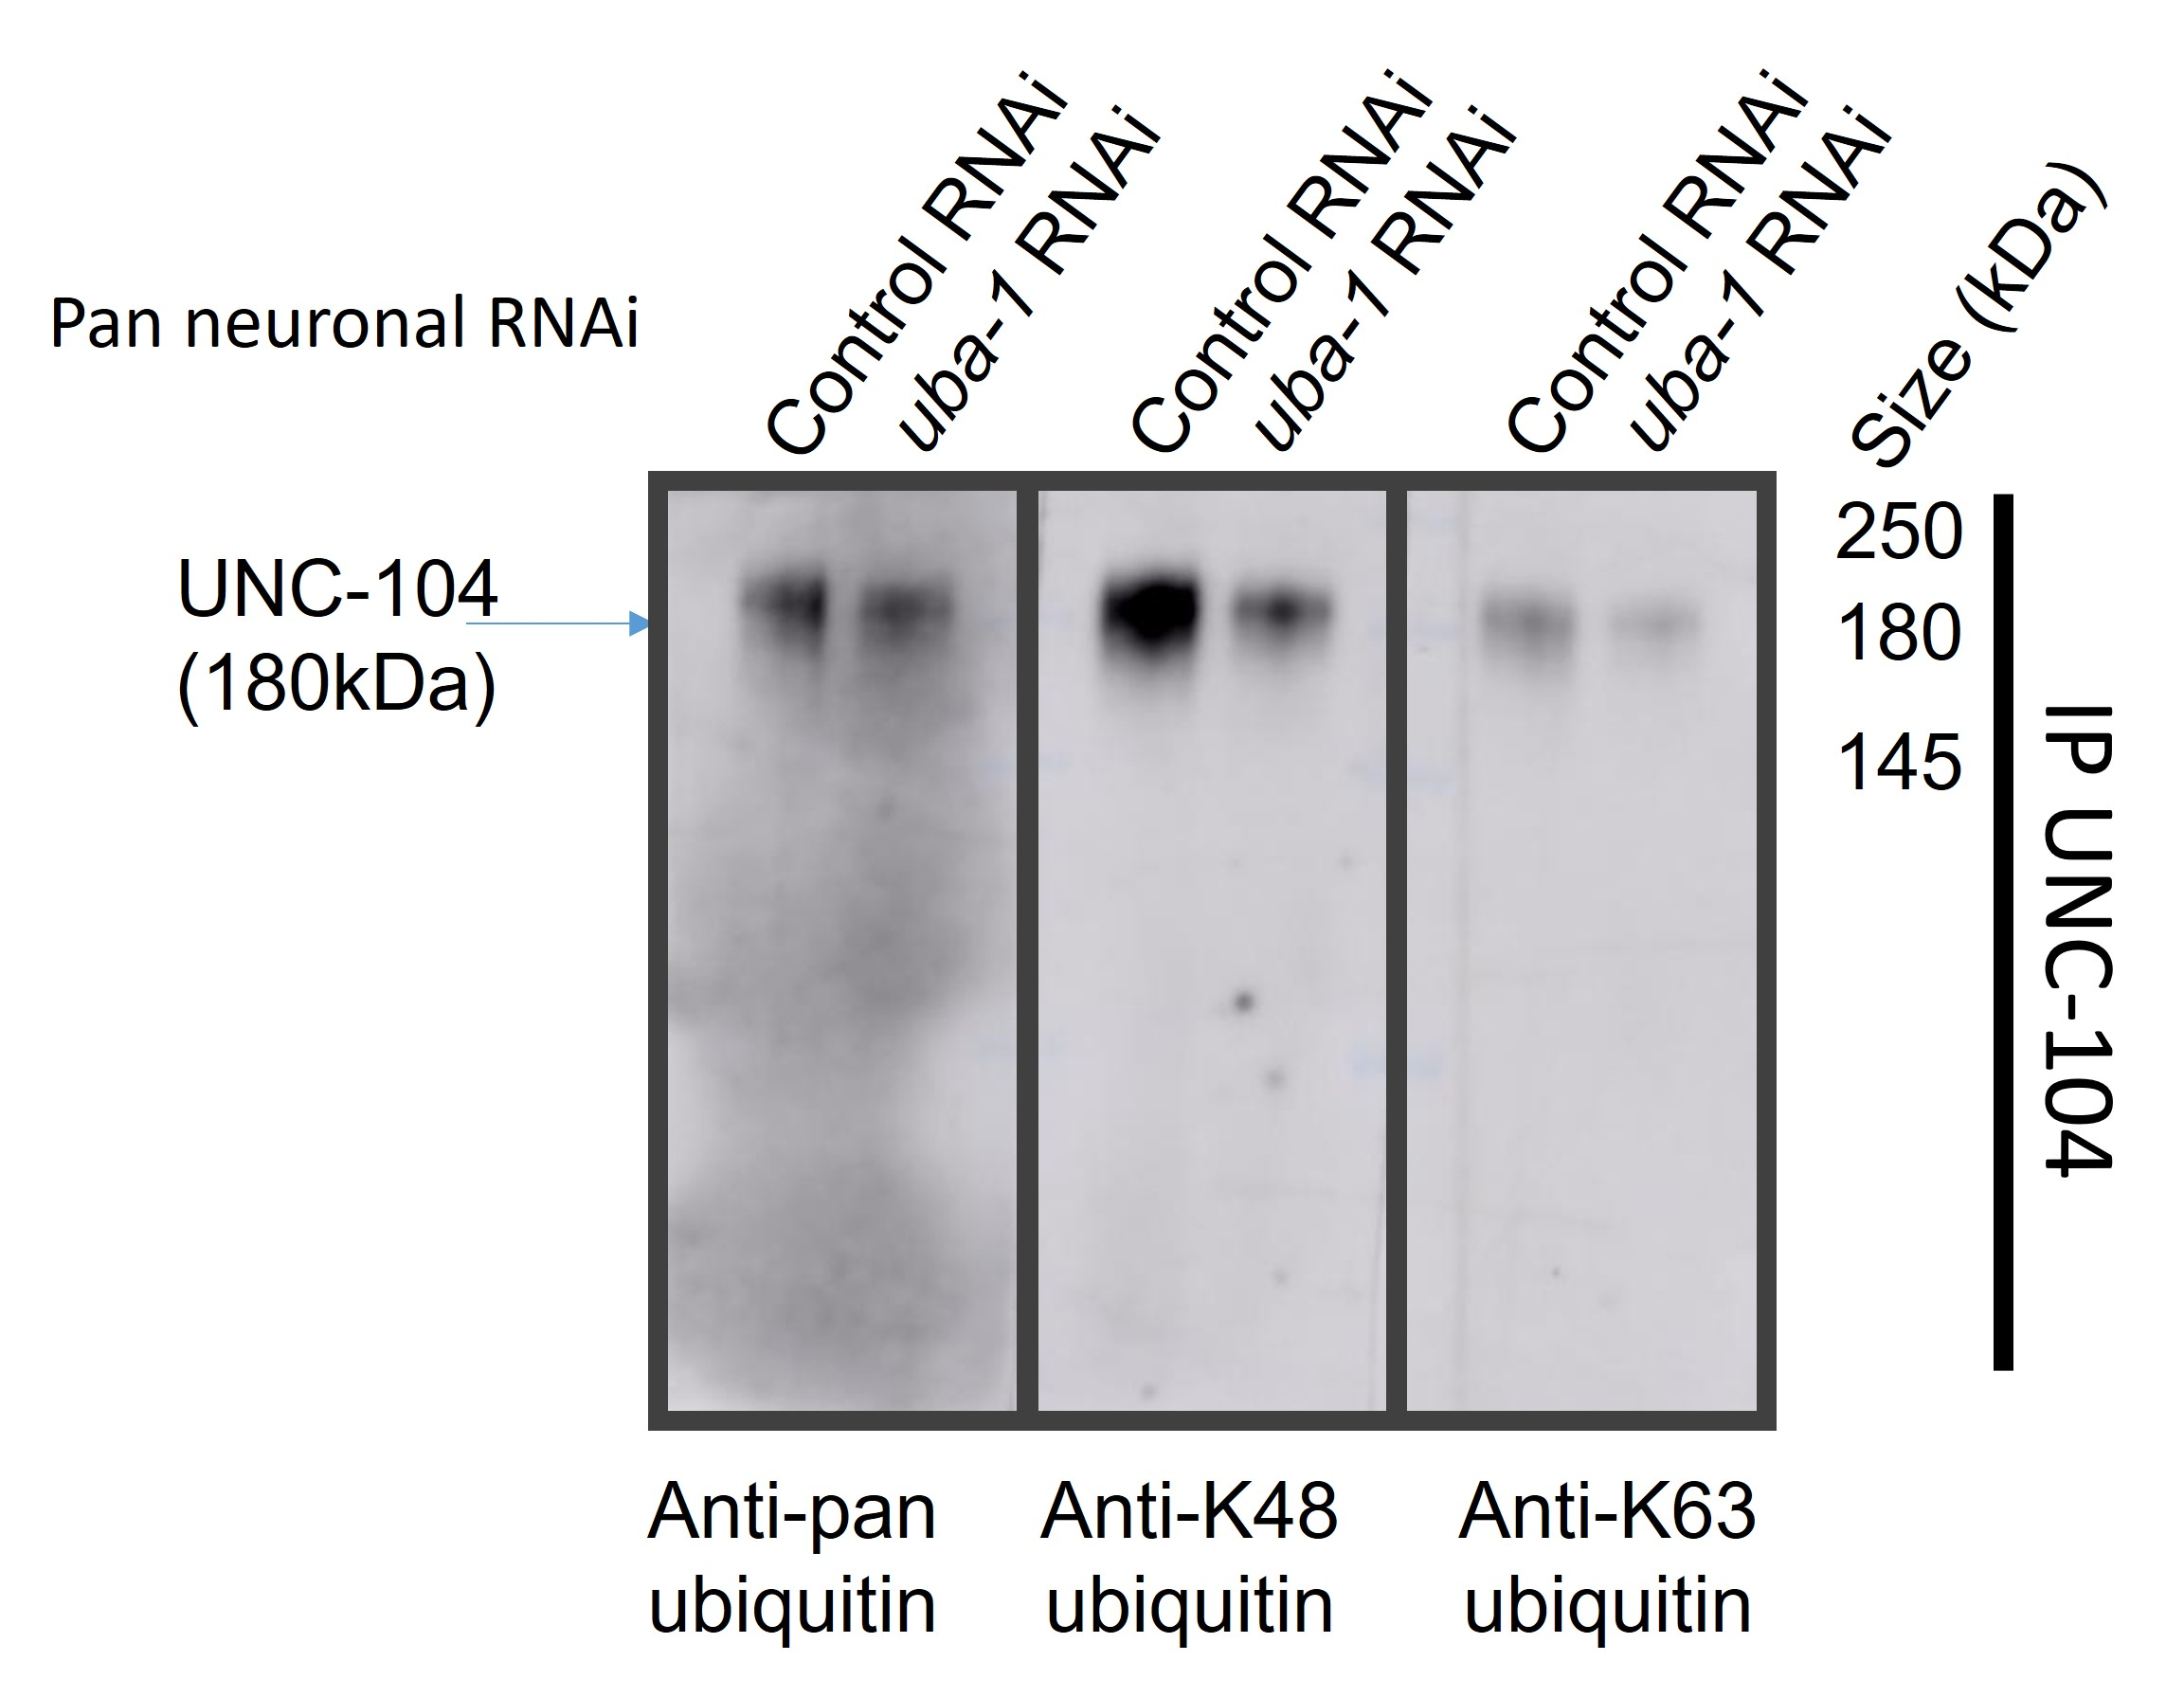
\includegraphics[width=\textwidth]{figs/example}
			
		\end{subfigure}
	\end{minipage}
	\begin{minipage}[t]{0.38\textwidth}
		\vspace{0pt}
		\caption[Increase in actin dynamics post injury in \textit{unc-16(lf)} depends on \textit{dlk-1}.]{\textbf{Increase in actin dynamics post injury in \textit{unc-16(lf)} depends on \textit{dlk-1}.}} \raggedright \small  A) Number, B) polymerization length, C) anterograde polymerization speed and D) number of stationary clusters assessed using GFP::utCH in uncut (U), and 3 hrs post ablation (3) in wild type, \textit{cebp-1(lf)}, \textit{dlk-1(null)}, \textit{unc-16(lf)}, or their doubles in the anterograde (black) and retrograde (gray) directions. Bar graphs represent the average of at least 15 animals with the whiskers representing S.E.M. One-way ANOVA was used for statistical analysis with all comparisons made with the respective time point in wild type animals. **p$<$0.01, ***p$<$0.001.
		\label{fig:Actdynmut}
	\end{minipage}
	\end{figure}
	
	\section{Discussion}
	
	These data together suggest that \textit{unc-16} may regulate microtubule dynamics post injury partially via DLK-1 dependent CEBP-1 signaling to the nucleus, and that the baseline microtubule dynamics are regulated largely independent of \textit{dlk-1}. Increased baseline microtubule dynamics may occur via DLK-1 independent role of UNC-16. In contrast, increased actin dynamics in \textit{unc-16(lf)} animals post injury may almost wholly depend on DLK-1 dependent CEBP-1 signaling, and the stationary actin clusters may be regulated independently via \textit{unc-16} and \textit{cebp-1}. Further, various features of actin and microtubule dynamics change faithfully 3 hours post injury, suggesting that this time scale is required for the neuron to sense and execute a regeneration program. This regeneration program likely undergoes pre-defined steps in a particular order, since both actin and microtubule polymerizing lengths increase before the number of polymerizing tracks are observed to increase. It will be interesting to understand how such different polymers are coordinated post injury to initiate and extend regrowth of the injured neuronal process.
	
	\newcolumntype{L}{>{\RaggedRight\hangafter=1\hangindent=1.5em}X}
	\begin{table}[H]\centering
		\caption{Strain list used in this study}\label{tab:StrainlistC}
		\scriptsize
		\begin{tabularx}{1\textwidth}{@{} l l L l @{}}\toprule
			S. No. &Strain name &Genotype &Reference \\\midrule
			1 &CZ8920 &\textit{cebp-1(tm2807)} abbreviated as \textit{cebp-1(lf)} &\cite{yan2009} \\
			2 &TT130 &\textit{unc-16(tb109)} abbreviated as \textit{unc-16(lf)} &\cite{choudhary2017} \\
			3 &CZ18975 &\textit{juIs338} [\textit{mec-4p}::\textit{ebp-2}::GFP] &\cite{ghosh-roy2012} \\
			4 & &\textit{wyIs291}[\textit{unc-86p}::GFP::\textit{utCH}] &\cite{chia2014} \\
			5 &CZ16351 &\textit{dlk-1(tm4024)} abbreviated as \textit{dlk-1(null)} &\cite{yan2009} \\
			6 &CZ14907 &\textit{rgef-1p}::\textit{dlk-1(L)}(\textit{juSi50}) referred to as DLK-1L in text and Mi(L) in figures &\cite{yan2012} \\
			\bottomrule
		\end{tabularx}
	\end{table}
	
	\begin{table}[H]\centering
		\caption{Primer list used in this study}\label{tab:PrimerlistC}
		\scriptsize
		\begin{tabularx}{1\textwidth}{@{} l l l l L @{}}\toprule
			S. No. &Primer TT no. &Primer name &Primer sequence &Amplicons expected \\\midrule
			1 &TTpr44 &cebp-1 (tm2807) FP &TCTGACGGCATCATTGTTCC &\multirow{2}{\hsize}{908 bp (WT) 425bp (mutant)} \\
			2 &TTpr45 &cebp-1 (tm2807) RP &ATTTCTCATCGCCTCTCACC & \\ \hline
			3 &TTpr48 &dlk-tm4024-f &CCCTGATTTTTAGCTTTGTCG &1079 bp for WT \\
			4 &TTpr49 &dlk-tm4024-r &CATTTGGAGTTGTGCTCTGG &619 bp for dlk-1(tm4024) \\ \hline
			5 &TTpr157 &b-juSi L-F &TCACCAATCACCACCTACAG &\multirow{2}{\hsize}{900bp for genomic dlk-1, 300bp for cDNA insertion in juSi50 } \\
			6 &TTpr158 &b-juSi L-R &CATTGGTGGATTAGGGCTTG & \\ \hline
			7 &TTpr159 &c-ttTi5605-f &GAGATTCTTGAAGACGACGAG &\multirow{2}{\hsize}{juSi50- no band, WT - 350 bp, (700bp non-specific band)} \\
			8 &TTpr160 &c-ttTi5605-r &TCTTGATAAGGAGTTCCACG & \\
			\bottomrule
		\end{tabularx}
	\end{table}
	
\end{appendices}
